\documentclass[twoside]{book}

% Packages required by doxygen
\usepackage{fixltx2e}
\usepackage{calc}
\usepackage{doxygen}
\usepackage[export]{adjustbox} % also loads graphicx
\usepackage{graphicx}
\usepackage[utf8]{inputenc}
\usepackage{makeidx}
\usepackage{multicol}
\usepackage{multirow}
\PassOptionsToPackage{warn}{textcomp}
\usepackage{textcomp}
\usepackage[nointegrals]{wasysym}
\usepackage[table]{xcolor}

% Font selection
\usepackage[T1]{fontenc}
\usepackage[scaled=.90]{helvet}
\usepackage{courier}
\usepackage{amssymb}
\usepackage{sectsty}
\renewcommand{\familydefault}{\sfdefault}
\allsectionsfont{%
  \fontseries{bc}\selectfont%
  \color{darkgray}%
}
\renewcommand{\DoxyLabelFont}{%
  \fontseries{bc}\selectfont%
  \color{darkgray}%
}
\newcommand{\+}{\discretionary{\mbox{\scriptsize$\hookleftarrow$}}{}{}}

% Page & text layout
\usepackage{geometry}
\geometry{%
  a4paper,%
  top=2.5cm,%
  bottom=2.5cm,%
  left=2.5cm,%
  right=2.5cm%
}
\tolerance=750
\hfuzz=15pt
\hbadness=750
\setlength{\emergencystretch}{15pt}
\setlength{\parindent}{0cm}
\setlength{\parskip}{3ex plus 2ex minus 2ex}
\makeatletter
\renewcommand{\paragraph}{%
  \@startsection{paragraph}{4}{0ex}{-1.0ex}{1.0ex}{%
    \normalfont\normalsize\bfseries\SS@parafont%
  }%
}
\renewcommand{\subparagraph}{%
  \@startsection{subparagraph}{5}{0ex}{-1.0ex}{1.0ex}{%
    \normalfont\normalsize\bfseries\SS@subparafont%
  }%
}
\makeatother

% Headers & footers
\usepackage{fancyhdr}
\pagestyle{fancyplain}
\fancyhead[LE]{\fancyplain{}{\bfseries\thepage}}
\fancyhead[CE]{\fancyplain{}{}}
\fancyhead[RE]{\fancyplain{}{\bfseries\leftmark}}
\fancyhead[LO]{\fancyplain{}{\bfseries\rightmark}}
\fancyhead[CO]{\fancyplain{}{}}
\fancyhead[RO]{\fancyplain{}{\bfseries\thepage}}
\fancyfoot[LE]{\fancyplain{}{}}
\fancyfoot[CE]{\fancyplain{}{}}
\fancyfoot[RE]{\fancyplain{}{\bfseries\scriptsize Generated by Doxygen }}
\fancyfoot[LO]{\fancyplain{}{\bfseries\scriptsize Generated by Doxygen }}
\fancyfoot[CO]{\fancyplain{}{}}
\fancyfoot[RO]{\fancyplain{}{}}
\renewcommand{\footrulewidth}{0.4pt}
\renewcommand{\chaptermark}[1]{%
  \markboth{#1}{}%
}
\renewcommand{\sectionmark}[1]{%
  \markright{\thesection\ #1}%
}

% Indices & bibliography
\usepackage{natbib}
\usepackage[titles]{tocloft}
\setcounter{tocdepth}{3}
\setcounter{secnumdepth}{5}
\makeindex

% Hyperlinks (required, but should be loaded last)
\usepackage{ifpdf}
\ifpdf
  \usepackage[pdftex,pagebackref=true]{hyperref}
\else
  \usepackage[ps2pdf,pagebackref=true]{hyperref}
\fi
\hypersetup{%
  colorlinks=true,%
  linkcolor=blue,%
  citecolor=blue,%
  unicode%
}

% Custom commands
\newcommand{\clearemptydoublepage}{%
  \newpage{\pagestyle{empty}\cleardoublepage}%
}

\usepackage{caption}
\captionsetup{labelsep=space,justification=centering,font={bf},singlelinecheck=off,skip=4pt,position=top}

%===== C O N T E N T S =====

\begin{document}

% Titlepage & ToC
\hypersetup{pageanchor=false,
             bookmarksnumbered=true,
             pdfencoding=unicode
            }
\pagenumbering{roman}
\begin{titlepage}
\vspace*{7cm}
\begin{center}%
{\Large C\+S354R Final Project \+: F\+PS Using Custom Open\+GL 3.3 Renderer \char`\"{}\+Larp\char`\"{} }\\
\vspace*{1cm}
{\large Generated by Doxygen 1.8.11}\\
\end{center}
\end{titlepage}
\clearemptydoublepage
\tableofcontents
\clearemptydoublepage
\pagenumbering{arabic}
\hypersetup{pageanchor=true}

%--- Begin generated contents ---
\chapter{Namespace Index}
\section{Namespace List}
Here is a list of all namespaces with brief descriptions\+:\begin{DoxyCompactList}
\item\contentsline{section}{\hyperlink{namespaceLarp}{Larp} }{\pageref{namespaceLarp}}{}
\end{DoxyCompactList}

\chapter{Class Index}
\section{Class List}
Here are the classes, structs, unions and interfaces with brief descriptions\+:\begin{DoxyCompactList}
\item\contentsline{section}{\hyperlink{classCamera}{Camera} }{\pageref{classCamera}}{}
\item\contentsline{section}{\hyperlink{classLarp_1_1ConfigurationLoader}{Larp\+::\+Configuration\+Loader} }{\pageref{classLarp_1_1ConfigurationLoader}}{}
\item\contentsline{section}{\hyperlink{classLarp_1_1Entity}{Larp\+::\+Entity} }{\pageref{classLarp_1_1Entity}}{}
\item\contentsline{section}{\hyperlink{classLarp_1_1Mesh}{Larp\+::\+Mesh} }{\pageref{classLarp_1_1Mesh}}{}
\item\contentsline{section}{\hyperlink{classLarp_1_1Model}{Larp\+::\+Model} }{\pageref{classLarp_1_1Model}}{}
\item\contentsline{section}{\hyperlink{classLarp_1_1Node}{Larp\+::\+Node} }{\pageref{classLarp_1_1Node}}{}
\item\contentsline{section}{\hyperlink{classLarp_1_1SceneGraph}{Larp\+::\+Scene\+Graph} }{\pageref{classLarp_1_1SceneGraph}}{}
\item\contentsline{section}{\hyperlink{classLarp_1_1Shader}{Larp\+::\+Shader} }{\pageref{classLarp_1_1Shader}}{}
\item\contentsline{section}{\hyperlink{classLarp_1_1Texture}{Larp\+::\+Texture} }{\pageref{classLarp_1_1Texture}}{}
\item\contentsline{section}{\hyperlink{structLarp_1_1Vertex}{Larp\+::\+Vertex} }{\pageref{structLarp_1_1Vertex}}{}
\end{DoxyCompactList}

\chapter{File Index}
\section{File List}
Here is a list of all files with brief descriptions\+:\begin{DoxyCompactList}
\item\contentsline{section}{src/\hyperlink{Camera_8cpp}{Camera.\+cpp} }{\pageref{Camera_8cpp}}{}
\item\contentsline{section}{src/\hyperlink{Camera_8hpp}{Camera.\+hpp} }{\pageref{Camera_8hpp}}{}
\item\contentsline{section}{src/\hyperlink{Entity_8cpp}{Entity.\+cpp} }{\pageref{Entity_8cpp}}{}
\item\contentsline{section}{src/\hyperlink{Entity_8hpp}{Entity.\+hpp} }{\pageref{Entity_8hpp}}{}
\item\contentsline{section}{src/\hyperlink{Error_8hpp}{Error.\+hpp} }{\pageref{Error_8hpp}}{}
\item\contentsline{section}{src/\hyperlink{Mesh_8cpp}{Mesh.\+cpp} }{\pageref{Mesh_8cpp}}{}
\item\contentsline{section}{src/\hyperlink{Mesh_8hpp}{Mesh.\+hpp} }{\pageref{Mesh_8hpp}}{}
\item\contentsline{section}{src/\hyperlink{Model_8cpp}{Model.\+cpp} }{\pageref{Model_8cpp}}{}
\item\contentsline{section}{src/\hyperlink{Model_8hpp}{Model.\+hpp} }{\pageref{Model_8hpp}}{}
\item\contentsline{section}{src/\hyperlink{Node_8cpp}{Node.\+cpp} }{\pageref{Node_8cpp}}{}
\item\contentsline{section}{src/\hyperlink{Node_8hpp}{Node.\+hpp} }{\pageref{Node_8hpp}}{}
\item\contentsline{section}{src/\hyperlink{RootNode_8hpp}{Root\+Node.\+hpp} }{\pageref{RootNode_8hpp}}{}
\item\contentsline{section}{src/\hyperlink{SceneGraph_8cpp}{Scene\+Graph.\+cpp} }{\pageref{SceneGraph_8cpp}}{}
\item\contentsline{section}{src/\hyperlink{SceneGraph_8hpp}{Scene\+Graph.\+hpp} }{\pageref{SceneGraph_8hpp}}{}
\item\contentsline{section}{src/\hyperlink{Shader_8cpp}{Shader.\+cpp} }{\pageref{Shader_8cpp}}{}
\item\contentsline{section}{src/\hyperlink{Shader_8hpp}{Shader.\+hpp} }{\pageref{Shader_8hpp}}{}
\item\contentsline{section}{src/\hyperlink{test_8cpp}{test.\+cpp} }{\pageref{test_8cpp}}{}
\end{DoxyCompactList}

\chapter{Namespace Documentation}
\hypertarget{namespaceLarp}{\section{Larp Namespace Reference}
\label{namespaceLarp}\index{Larp@{Larp}}
}
\subsection*{Classes}
\begin{DoxyCompactItemize}
\item 
class \hyperlink{classLarp_1_1ConfigurationLoader}{Configuration\-Loader}
\item 
class \hyperlink{classLarp_1_1Entity}{Entity}
\item 
struct \hyperlink{structLarp_1_1Vertex}{Vertex}
\item 
class \hyperlink{classLarp_1_1Texture}{Texture}
\item 
class \hyperlink{classLarp_1_1Mesh}{Mesh}
\item 
class \hyperlink{classLarp_1_1Model}{Model}
\item 
class \hyperlink{classLarp_1_1Node}{Node}
\item 
class \hyperlink{classLarp_1_1SceneGraph}{Scene\-Graph}
\item 
class \hyperlink{classLarp_1_1Shader}{Shader}
\end{DoxyCompactItemize}
\subsection*{Typedefs}
\begin{DoxyCompactItemize}
\item 
typedef std\-::shared\-\_\-ptr$<$ \hyperlink{classLarp_1_1Entity}{Entity} $>$ \hyperlink{namespaceLarp_ae3ffca1f126e4263cbdc59b116ee465a}{Shared\-Entity}
\item 
typedef std\-::unique\-\_\-ptr$<$ \hyperlink{classLarp_1_1Entity}{Entity} $>$ \hyperlink{namespaceLarp_ad6d203c6dc3d8ea7a5517a64e1665403}{Unique\-Entity}
\item 
typedef \hyperlink{classLarp_1_1Entity}{Entity} $\ast$const \hyperlink{namespaceLarp_a775efcc4cabb308d50168c52df343353}{Entity\-Ptr}
\item 
typedef std\-::unique\-\_\-ptr$<$ \hyperlink{classLarp_1_1Node}{Node} $>$ \hyperlink{namespaceLarp_ad95a88bc34f8c78cefd64c9bbeb94a58}{Unique\-Node}
\item 
typedef \hyperlink{classLarp_1_1Node}{Node} $\ast$const \hyperlink{namespaceLarp_a171c1dc8b70cfb441b15d7386780db23}{Node\-Ptr}
\item 
typedef std\-::unique\-\_\-ptr\\*
$<$ \hyperlink{classLarp_1_1SceneGraph}{Scene\-Graph} $>$ \hyperlink{namespaceLarp_a81a0d129ec1fc8f1f9fa231fbba6b19b}{Unique\-Scene\-Graph}
\item 
typedef \hyperlink{classLarp_1_1SceneGraph}{Scene\-Graph} $\ast$const \hyperlink{namespaceLarp_acf02d81e4b52238dcd17cb6249eadadc}{Scene\-Graph\-Ptr}
\end{DoxyCompactItemize}


\subsection{Typedef Documentation}
\hypertarget{namespaceLarp_a775efcc4cabb308d50168c52df343353}{\index{Larp@{Larp}!Entity\-Ptr@{Entity\-Ptr}}
\index{Entity\-Ptr@{Entity\-Ptr}!Larp@{Larp}}
\subsubsection[{Entity\-Ptr}]{\setlength{\rightskip}{0pt plus 5cm}typedef {\bf Entity}$\ast$ const {\bf Larp\-::\-Entity\-Ptr}}}\label{namespaceLarp_a775efcc4cabb308d50168c52df343353}
\hypertarget{namespaceLarp_a171c1dc8b70cfb441b15d7386780db23}{\index{Larp@{Larp}!Node\-Ptr@{Node\-Ptr}}
\index{Node\-Ptr@{Node\-Ptr}!Larp@{Larp}}
\subsubsection[{Node\-Ptr}]{\setlength{\rightskip}{0pt plus 5cm}typedef {\bf Node}$\ast$ const {\bf Larp\-::\-Node\-Ptr}}}\label{namespaceLarp_a171c1dc8b70cfb441b15d7386780db23}
\hypertarget{namespaceLarp_acf02d81e4b52238dcd17cb6249eadadc}{\index{Larp@{Larp}!Scene\-Graph\-Ptr@{Scene\-Graph\-Ptr}}
\index{Scene\-Graph\-Ptr@{Scene\-Graph\-Ptr}!Larp@{Larp}}
\subsubsection[{Scene\-Graph\-Ptr}]{\setlength{\rightskip}{0pt plus 5cm}typedef {\bf Scene\-Graph}$\ast$ const {\bf Larp\-::\-Scene\-Graph\-Ptr}}}\label{namespaceLarp_acf02d81e4b52238dcd17cb6249eadadc}
\hypertarget{namespaceLarp_ae3ffca1f126e4263cbdc59b116ee465a}{\index{Larp@{Larp}!Shared\-Entity@{Shared\-Entity}}
\index{Shared\-Entity@{Shared\-Entity}!Larp@{Larp}}
\subsubsection[{Shared\-Entity}]{\setlength{\rightskip}{0pt plus 5cm}typedef std\-::shared\-\_\-ptr$<${\bf Entity}$>$ {\bf Larp\-::\-Shared\-Entity}}}\label{namespaceLarp_ae3ffca1f126e4263cbdc59b116ee465a}
\hypertarget{namespaceLarp_ad6d203c6dc3d8ea7a5517a64e1665403}{\index{Larp@{Larp}!Unique\-Entity@{Unique\-Entity}}
\index{Unique\-Entity@{Unique\-Entity}!Larp@{Larp}}
\subsubsection[{Unique\-Entity}]{\setlength{\rightskip}{0pt plus 5cm}typedef std\-::unique\-\_\-ptr$<${\bf Entity}$>$ {\bf Larp\-::\-Unique\-Entity}}}\label{namespaceLarp_ad6d203c6dc3d8ea7a5517a64e1665403}
\hypertarget{namespaceLarp_ad95a88bc34f8c78cefd64c9bbeb94a58}{\index{Larp@{Larp}!Unique\-Node@{Unique\-Node}}
\index{Unique\-Node@{Unique\-Node}!Larp@{Larp}}
\subsubsection[{Unique\-Node}]{\setlength{\rightskip}{0pt plus 5cm}typedef std\-::unique\-\_\-ptr$<${\bf Node}$>$ {\bf Larp\-::\-Unique\-Node}}}\label{namespaceLarp_ad95a88bc34f8c78cefd64c9bbeb94a58}
\hypertarget{namespaceLarp_a81a0d129ec1fc8f1f9fa231fbba6b19b}{\index{Larp@{Larp}!Unique\-Scene\-Graph@{Unique\-Scene\-Graph}}
\index{Unique\-Scene\-Graph@{Unique\-Scene\-Graph}!Larp@{Larp}}
\subsubsection[{Unique\-Scene\-Graph}]{\setlength{\rightskip}{0pt plus 5cm}typedef std\-::unique\-\_\-ptr$<${\bf Scene\-Graph}$>$ {\bf Larp\-::\-Unique\-Scene\-Graph}}}\label{namespaceLarp_a81a0d129ec1fc8f1f9fa231fbba6b19b}

\chapter{Class Documentation}
\hypertarget{classCamera}{\section{Camera Class Reference}
\label{classCamera}\index{Camera@{Camera}}
}


{\ttfamily \#include $<$Camera.\-hpp$>$}

\subsection*{Public Types}
\begin{DoxyCompactItemize}
\item 
enum \hyperlink{classCamera_a9825f2bf1ddc209c3b2d336080d8407a}{Camera\-Movement} \{ \hyperlink{classCamera_a9825f2bf1ddc209c3b2d336080d8407aa6388b5408cf8440021383388044ae77f}{F\-O\-R\-W\-A\-R\-D}, 
\hyperlink{classCamera_a9825f2bf1ddc209c3b2d336080d8407aae18db08a2289896f26dcddf6e2ad274f}{B\-A\-C\-K\-W\-A\-R\-D}, 
\hyperlink{classCamera_a9825f2bf1ddc209c3b2d336080d8407aa1bed5588ea4c26163a72f0fc8621f6be}{L\-E\-F\-T}, 
\hyperlink{classCamera_a9825f2bf1ddc209c3b2d336080d8407aaedac3a8506bf2bae7df2d36dd5580884}{R\-I\-G\-H\-T}
 \}
\end{DoxyCompactItemize}
\subsection*{Public Member Functions}
\begin{DoxyCompactItemize}
\item 
\hyperlink{classCamera_a535f3a2413a88c2f1e7d1147bec0039c}{Camera} (glm\-::vec3 position=glm\-::vec3(0.\-0f, 0.\-0f, 0.\-0f), glm\-::vec3 up=glm\-::vec3(0.\-0f, 1.\-0f, 0.\-0f), G\-Lfloat yaw=\-Y\-A\-W, G\-Lfloat pitch=\-P\-I\-T\-C\-H)
\item 
\hyperlink{classCamera_af0f6ba09d293db5b1c6ba63d195cff57}{Camera} (G\-Lfloat pos\-\_\-x, G\-Lfloat pos\-\_\-y, G\-Lfloat pos\-\_\-z, G\-Lfloat up\-\_\-x, G\-Lfloat up\-\_\-y, G\-Lfloat up\-\_\-z, G\-Lfloat yaw=\hyperlink{classCamera_a79050e94e98c5c1cc0127c41edb4ed16}{Y\-A\-W}, G\-Lfloat pitch=\hyperlink{classCamera_afd43f32a47d2db8922dc32030fd84379}{P\-I\-T\-C\-H})
\item 
glm\-::mat4 \hyperlink{classCamera_aedac0150156798ae1880eabaa3b9f071}{get\-\_\-view\-\_\-matrix} ()
\item 
void \hyperlink{classCamera_ac32b5b8c93934f8faa8e8637dec855d4}{process\-\_\-keyboard} (\hyperlink{classCamera_a9825f2bf1ddc209c3b2d336080d8407a}{Camera\-Movement} direction, G\-Lfloat delta\-\_\-time)
\item 
void \hyperlink{classCamera_ab650c0e1f0c55582339623e7c3b4b10d}{process\-\_\-mouse\-\_\-movement} (G\-Lfloat x\-\_\-offset, G\-Lfloat y\-\_\-offset, G\-Lboolean constrain\-\_\-pitch=true)
\item 
void \hyperlink{classCamera_a9cb2efbeb1a0007f1ea908e3e74c92a1}{process\-\_\-mouse\-\_\-scroll} (G\-Lfloat y\-\_\-offset)
\end{DoxyCompactItemize}
\subsection*{Public Attributes}
\begin{DoxyCompactItemize}
\item 
glm\-::vec3 \hyperlink{classCamera_a0a931ed2051befaad1f482b3b5e98ca0}{\-\_\-position}
\item 
glm\-::vec3 \hyperlink{classCamera_ac610e748840c4b70c9081c2d68df2e8d}{\-\_\-front}
\item 
glm\-::vec3 \hyperlink{classCamera_a323a698e4c5773ee3ec380851b145e2d}{\-\_\-up}
\item 
glm\-::vec3 \hyperlink{classCamera_a4c556280ed181d8589c28eec7ebebb49}{\-\_\-right}
\item 
glm\-::vec3 \hyperlink{classCamera_aa5d721a01ba1cb41eafb02e39ea29e03}{\-\_\-world\-\_\-up}
\item 
G\-Lfloat \hyperlink{classCamera_ab815461cc043db1f5810c2f488641740}{\-\_\-yaw}
\item 
G\-Lfloat \hyperlink{classCamera_a23a8b8859c44721d7082b89809318918}{\-\_\-pitch}
\item 
G\-Lfloat \hyperlink{classCamera_a6f31b5658310866d3228614a755b59b0}{\-\_\-movement\-\_\-speed}
\item 
G\-Lfloat \hyperlink{classCamera_aeb483d642e0bcf11aa881467ac9676fe}{\-\_\-mouse\-\_\-sensitivity}
\item 
G\-Lfloat \hyperlink{classCamera_a99dc4d95f58be2427ff6c8d93c676ecd}{\-\_\-zoom}
\end{DoxyCompactItemize}
\subsection*{Static Public Attributes}
\begin{DoxyCompactItemize}
\item 
static const G\-Lfloat \hyperlink{classCamera_a79050e94e98c5c1cc0127c41edb4ed16}{Y\-A\-W} = -\/90.\-0f
\item 
static const G\-Lfloat \hyperlink{classCamera_afd43f32a47d2db8922dc32030fd84379}{P\-I\-T\-C\-H} = 0.\-0f
\item 
static const G\-Lfloat \hyperlink{classCamera_acc2ddbb4a3bdb2829896703edf72ca1e}{S\-P\-E\-E\-D} = 3.\-0f
\item 
static const G\-Lfloat \hyperlink{classCamera_adee09ae2133f9fe95a6eb72a6cb8db20}{S\-E\-N\-S\-I\-T\-I\-V\-I\-T\-Y} = 0.\-25f
\item 
static const G\-Lfloat \hyperlink{classCamera_a34cdfe4c17868880037d5ff78159f158}{Z\-O\-O\-M} = 45.\-0f
\end{DoxyCompactItemize}
\subsection*{Private Member Functions}
\begin{DoxyCompactItemize}
\item 
void \hyperlink{classCamera_ad9745a585d867bc34439c36f0a6d66a1}{update\-\_\-camera\-\_\-vectors} ()
\end{DoxyCompactItemize}


\subsection{Detailed Description}
An abstract camera class that processes input and calculates the corresponding Eular Angles, Vectors and Matrices for use in Open\-G\-L 

\subsection{Member Enumeration Documentation}
\hypertarget{classCamera_a9825f2bf1ddc209c3b2d336080d8407a}{\index{Camera@{Camera}!Camera\-Movement@{Camera\-Movement}}
\index{Camera\-Movement@{Camera\-Movement}!Camera@{Camera}}
\subsubsection[{Camera\-Movement}]{\setlength{\rightskip}{0pt plus 5cm}enum {\bf Camera\-::\-Camera\-Movement}}}\label{classCamera_a9825f2bf1ddc209c3b2d336080d8407a}
Enum that defines several directions for the \hyperlink{classCamera}{Camera} to move \begin{Desc}
\item[Enumerator]\par
\begin{description}
\index{F\-O\-R\-W\-A\-R\-D@{F\-O\-R\-W\-A\-R\-D}!Camera@{Camera}}\index{Camera@{Camera}!F\-O\-R\-W\-A\-R\-D@{F\-O\-R\-W\-A\-R\-D}}\item[{\em 
\hypertarget{classCamera_a9825f2bf1ddc209c3b2d336080d8407aa6388b5408cf8440021383388044ae77f}{F\-O\-R\-W\-A\-R\-D}\label{classCamera_a9825f2bf1ddc209c3b2d336080d8407aa6388b5408cf8440021383388044ae77f}
}]\index{B\-A\-C\-K\-W\-A\-R\-D@{B\-A\-C\-K\-W\-A\-R\-D}!Camera@{Camera}}\index{Camera@{Camera}!B\-A\-C\-K\-W\-A\-R\-D@{B\-A\-C\-K\-W\-A\-R\-D}}\item[{\em 
\hypertarget{classCamera_a9825f2bf1ddc209c3b2d336080d8407aae18db08a2289896f26dcddf6e2ad274f}{B\-A\-C\-K\-W\-A\-R\-D}\label{classCamera_a9825f2bf1ddc209c3b2d336080d8407aae18db08a2289896f26dcddf6e2ad274f}
}]\index{L\-E\-F\-T@{L\-E\-F\-T}!Camera@{Camera}}\index{Camera@{Camera}!L\-E\-F\-T@{L\-E\-F\-T}}\item[{\em 
\hypertarget{classCamera_a9825f2bf1ddc209c3b2d336080d8407aa1bed5588ea4c26163a72f0fc8621f6be}{L\-E\-F\-T}\label{classCamera_a9825f2bf1ddc209c3b2d336080d8407aa1bed5588ea4c26163a72f0fc8621f6be}
}]\index{R\-I\-G\-H\-T@{R\-I\-G\-H\-T}!Camera@{Camera}}\index{Camera@{Camera}!R\-I\-G\-H\-T@{R\-I\-G\-H\-T}}\item[{\em 
\hypertarget{classCamera_a9825f2bf1ddc209c3b2d336080d8407aaedac3a8506bf2bae7df2d36dd5580884}{R\-I\-G\-H\-T}\label{classCamera_a9825f2bf1ddc209c3b2d336080d8407aaedac3a8506bf2bae7df2d36dd5580884}
}]\end{description}
\end{Desc}


\subsection{Constructor \& Destructor Documentation}
\hypertarget{classCamera_a535f3a2413a88c2f1e7d1147bec0039c}{\index{Camera@{Camera}!Camera@{Camera}}
\index{Camera@{Camera}!Camera@{Camera}}
\subsubsection[{Camera}]{\setlength{\rightskip}{0pt plus 5cm}Camera\-::\-Camera (
\begin{DoxyParamCaption}
\item[{glm\-::vec3}]{position = {\ttfamily glm\-:\-:vec3(0.0f,~0.0f,~0.0f)}, }
\item[{glm\-::vec3}]{up = {\ttfamily glm\-:\-:vec3(0.0f,~1.0f,~0.0f)}, }
\item[{G\-Lfloat}]{yaw = {\ttfamily {\bf Y\-A\-W}}, }
\item[{G\-Lfloat}]{pitch = {\ttfamily {\bf P\-I\-T\-C\-H}}}
\end{DoxyParamCaption}
)}}\label{classCamera_a535f3a2413a88c2f1e7d1147bec0039c}
Constructor 
\begin{DoxyParams}{Parameters}
{\em position} & The starting position of the \hyperlink{classCamera}{Camera} as a glm\-::vec3. If not provided the \hyperlink{classCamera}{Camera} will be centered at the origin. \\
\hline
{\em up} & The up vector for the world. If not provided the y-\/axis will be used as the world up vector \\
\hline
{\em yaw} & The initial yaw for the \hyperlink{classCamera}{Camera}. If not provided, the \hyperlink{classCamera}{Camera} will start pointing down the -\/z-\/axis \\
\hline
{\em pitch} & The initial pitch of the \hyperlink{classCamera}{Camera}. If not provided, the \hyperlink{classCamera}{Camera} will start on the xz-\/plane \\
\hline
\end{DoxyParams}
\hypertarget{classCamera_af0f6ba09d293db5b1c6ba63d195cff57}{\index{Camera@{Camera}!Camera@{Camera}}
\index{Camera@{Camera}!Camera@{Camera}}
\subsubsection[{Camera}]{\setlength{\rightskip}{0pt plus 5cm}Camera\-::\-Camera (
\begin{DoxyParamCaption}
\item[{G\-Lfloat}]{pos\-\_\-x, }
\item[{G\-Lfloat}]{pos\-\_\-y, }
\item[{G\-Lfloat}]{pos\-\_\-z, }
\item[{G\-Lfloat}]{up\-\_\-x, }
\item[{G\-Lfloat}]{up\-\_\-y, }
\item[{G\-Lfloat}]{up\-\_\-z, }
\item[{G\-Lfloat}]{yaw = {\ttfamily {\bf Y\-A\-W}}, }
\item[{G\-Lfloat}]{pitch = {\ttfamily {\bf P\-I\-T\-C\-H}}}
\end{DoxyParamCaption}
)}}\label{classCamera_af0f6ba09d293db5b1c6ba63d195cff57}
Constructor 
\begin{DoxyParams}{Parameters}
{\em pos\-\_\-x} & The starting x position of the \hyperlink{classCamera}{Camera}. \\
\hline
{\em pos\-\_\-y} & The starting y position of the \hyperlink{classCamera}{Camera}. \\
\hline
{\em pos\-\_\-z} & The starting z position of the \hyperlink{classCamera}{Camera}. \\
\hline
{\em up\-\_\-x} & The x-\/value of the world up vector of the \hyperlink{classCamera}{Camera}. \\
\hline
{\em up\-\_\-y} & The y-\/value of the world up vector of the \hyperlink{classCamera}{Camera}. \\
\hline
{\em up\-\_\-z} & The z-\/value of the world up vector of the \hyperlink{classCamera}{Camera}. \\
\hline
{\em yaw} & The initial yaw for the \hyperlink{classCamera}{Camera}. If not provided, the \hyperlink{classCamera}{Camera} will start pointing down the -\/z-\/axis \\
\hline
{\em pitch} & The initial pitch of the \hyperlink{classCamera}{Camera}. If not provided, the \hyperlink{classCamera}{Camera} will start on the xz-\/plane \\
\hline
\end{DoxyParams}


\subsection{Member Function Documentation}
\hypertarget{classCamera_aedac0150156798ae1880eabaa3b9f071}{\index{Camera@{Camera}!get\-\_\-view\-\_\-matrix@{get\-\_\-view\-\_\-matrix}}
\index{get\-\_\-view\-\_\-matrix@{get\-\_\-view\-\_\-matrix}!Camera@{Camera}}
\subsubsection[{get\-\_\-view\-\_\-matrix}]{\setlength{\rightskip}{0pt plus 5cm}glm\-::mat4 Camera\-::get\-\_\-view\-\_\-matrix (
\begin{DoxyParamCaption}
{}
\end{DoxyParamCaption}
)}}\label{classCamera_aedac0150156798ae1880eabaa3b9f071}
\begin{DoxyReturn}{Returns}
the view matrix calculated using Euler angles and the look\-At matrix 
\end{DoxyReturn}
\hypertarget{classCamera_ac32b5b8c93934f8faa8e8637dec855d4}{\index{Camera@{Camera}!process\-\_\-keyboard@{process\-\_\-keyboard}}
\index{process\-\_\-keyboard@{process\-\_\-keyboard}!Camera@{Camera}}
\subsubsection[{process\-\_\-keyboard}]{\setlength{\rightskip}{0pt plus 5cm}void Camera\-::process\-\_\-keyboard (
\begin{DoxyParamCaption}
\item[{{\bf Camera\-Movement}}]{direction, }
\item[{G\-Lfloat}]{delta\-\_\-time}
\end{DoxyParamCaption}
)}}\label{classCamera_ac32b5b8c93934f8faa8e8637dec855d4}
Processes input received from any keyboard-\/like input system. 
\begin{DoxyParams}{Parameters}
{\em direction} & A direction to move the \hyperlink{classCamera}{Camera}. Must be one of the directions predefined in the Camera\-Movement enum. \\
\hline
{\em delta\-\_\-time} & The duration of time between frames. Used to avoid variable camera speeds \\
\hline
\end{DoxyParams}
\begin{DoxySeeAlso}{See Also}
\hyperlink{classCamera_a9825f2bf1ddc209c3b2d336080d8407a}{Camera\-Movement} 
\end{DoxySeeAlso}

\begin{DoxyExceptions}{Exceptions}
{\em std\-::runtime\-\_\-error} & whenever direction is not one of those defined by Camera\-Movement \\
\hline
\end{DoxyExceptions}
\hypertarget{classCamera_ab650c0e1f0c55582339623e7c3b4b10d}{\index{Camera@{Camera}!process\-\_\-mouse\-\_\-movement@{process\-\_\-mouse\-\_\-movement}}
\index{process\-\_\-mouse\-\_\-movement@{process\-\_\-mouse\-\_\-movement}!Camera@{Camera}}
\subsubsection[{process\-\_\-mouse\-\_\-movement}]{\setlength{\rightskip}{0pt plus 5cm}void Camera\-::process\-\_\-mouse\-\_\-movement (
\begin{DoxyParamCaption}
\item[{G\-Lfloat}]{x\-\_\-offset, }
\item[{G\-Lfloat}]{y\-\_\-offset, }
\item[{G\-Lboolean}]{constrain\-\_\-pitch = {\ttfamily true}}
\end{DoxyParamCaption}
)}}\label{classCamera_ab650c0e1f0c55582339623e7c3b4b10d}
Processes input received from a mouse input system. 
\begin{DoxyParams}{Parameters}
{\em x\-\_\-offset} & The value used to update the \hyperlink{classCamera}{Camera}'s yaw. A positive x\-\_\-offset will yaw the \hyperlink{classCamera}{Camera} counter-\/clockwise. \\
\hline
{\em y\-\_\-offset} & The value used to update the \hyperlink{classCamera}{Camera}'s pitch. A positive y\-\_\-offset will pitch the \hyperlink{classCamera}{Camera} up. \\
\hline
{\em constrain\-\_\-pitch} & If true, the \hyperlink{classCamera}{Camera}'s pitch will be constrained to the range \mbox{[}-\/89.\-0, 89.\-0\mbox{]} degrees. Useful to avoid Gimbal lock. If not provided, the \hyperlink{classCamera}{Camera}'s pitch will be constrained \\
\hline
\end{DoxyParams}
\hypertarget{classCamera_a9cb2efbeb1a0007f1ea908e3e74c92a1}{\index{Camera@{Camera}!process\-\_\-mouse\-\_\-scroll@{process\-\_\-mouse\-\_\-scroll}}
\index{process\-\_\-mouse\-\_\-scroll@{process\-\_\-mouse\-\_\-scroll}!Camera@{Camera}}
\subsubsection[{process\-\_\-mouse\-\_\-scroll}]{\setlength{\rightskip}{0pt plus 5cm}void Camera\-::process\-\_\-mouse\-\_\-scroll (
\begin{DoxyParamCaption}
\item[{G\-Lfloat}]{y\-\_\-offset}
\end{DoxyParamCaption}
)}}\label{classCamera_a9cb2efbeb1a0007f1ea908e3e74c92a1}
Processes input received from a mouse scroll-\/wheel event. 
\begin{DoxyParams}{Parameters}
{\em y\-\_\-offset} & The offset of the input device used to zoom the camera. A positive offset zooms the camera in by reducing the F\-O\-V in degrees, while a negative offset zooms the camera out. \\
\hline
\end{DoxyParams}
\hypertarget{classCamera_ad9745a585d867bc34439c36f0a6d66a1}{\index{Camera@{Camera}!update\-\_\-camera\-\_\-vectors@{update\-\_\-camera\-\_\-vectors}}
\index{update\-\_\-camera\-\_\-vectors@{update\-\_\-camera\-\_\-vectors}!Camera@{Camera}}
\subsubsection[{update\-\_\-camera\-\_\-vectors}]{\setlength{\rightskip}{0pt plus 5cm}void Camera\-::update\-\_\-camera\-\_\-vectors (
\begin{DoxyParamCaption}
{}
\end{DoxyParamCaption}
)\hspace{0.3cm}{\ttfamily [private]}}}\label{classCamera_ad9745a585d867bc34439c36f0a6d66a1}
Calculates the front vector from the \hyperlink{classCamera}{Camera}'s (updated) Eular Angles 

\subsection{Member Data Documentation}
\hypertarget{classCamera_ac610e748840c4b70c9081c2d68df2e8d}{\index{Camera@{Camera}!\-\_\-front@{\-\_\-front}}
\index{\-\_\-front@{\-\_\-front}!Camera@{Camera}}
\subsubsection[{\-\_\-front}]{\setlength{\rightskip}{0pt plus 5cm}glm\-::vec3 Camera\-::\-\_\-front}}\label{classCamera_ac610e748840c4b70c9081c2d68df2e8d}
Vector representing which direction the \hyperlink{classCamera}{Camera} is facing. Used when calculating how the \hyperlink{classCamera}{Camera} moves forward and backward. \hypertarget{classCamera_aeb483d642e0bcf11aa881467ac9676fe}{\index{Camera@{Camera}!\-\_\-mouse\-\_\-sensitivity@{\-\_\-mouse\-\_\-sensitivity}}
\index{\-\_\-mouse\-\_\-sensitivity@{\-\_\-mouse\-\_\-sensitivity}!Camera@{Camera}}
\subsubsection[{\-\_\-mouse\-\_\-sensitivity}]{\setlength{\rightskip}{0pt plus 5cm}G\-Lfloat Camera\-::\-\_\-mouse\-\_\-sensitivity}}\label{classCamera_aeb483d642e0bcf11aa881467ac9676fe}
Determines how much the \hyperlink{classCamera}{Camera} rotates on mouse movement \hypertarget{classCamera_a6f31b5658310866d3228614a755b59b0}{\index{Camera@{Camera}!\-\_\-movement\-\_\-speed@{\-\_\-movement\-\_\-speed}}
\index{\-\_\-movement\-\_\-speed@{\-\_\-movement\-\_\-speed}!Camera@{Camera}}
\subsubsection[{\-\_\-movement\-\_\-speed}]{\setlength{\rightskip}{0pt plus 5cm}G\-Lfloat Camera\-::\-\_\-movement\-\_\-speed}}\label{classCamera_a6f31b5658310866d3228614a755b59b0}
Determines how fast the \hyperlink{classCamera}{Camera} moves \hypertarget{classCamera_a23a8b8859c44721d7082b89809318918}{\index{Camera@{Camera}!\-\_\-pitch@{\-\_\-pitch}}
\index{\-\_\-pitch@{\-\_\-pitch}!Camera@{Camera}}
\subsubsection[{\-\_\-pitch}]{\setlength{\rightskip}{0pt plus 5cm}G\-Lfloat Camera\-::\-\_\-pitch}}\label{classCamera_a23a8b8859c44721d7082b89809318918}
This \hyperlink{classCamera}{Camera}'s pitch in degrees \hypertarget{classCamera_a0a931ed2051befaad1f482b3b5e98ca0}{\index{Camera@{Camera}!\-\_\-position@{\-\_\-position}}
\index{\-\_\-position@{\-\_\-position}!Camera@{Camera}}
\subsubsection[{\-\_\-position}]{\setlength{\rightskip}{0pt plus 5cm}glm\-::vec3 Camera\-::\-\_\-position}}\label{classCamera_a0a931ed2051befaad1f482b3b5e98ca0}
Current position of the camera \hypertarget{classCamera_a4c556280ed181d8589c28eec7ebebb49}{\index{Camera@{Camera}!\-\_\-right@{\-\_\-right}}
\index{\-\_\-right@{\-\_\-right}!Camera@{Camera}}
\subsubsection[{\-\_\-right}]{\setlength{\rightskip}{0pt plus 5cm}glm\-::vec3 Camera\-::\-\_\-right}}\label{classCamera_a4c556280ed181d8589c28eec7ebebb49}
Vector representing the x-\/axis in view space. Also used to calculate how the \hyperlink{classCamera}{Camera} moves left and right. \hypertarget{classCamera_a323a698e4c5773ee3ec380851b145e2d}{\index{Camera@{Camera}!\-\_\-up@{\-\_\-up}}
\index{\-\_\-up@{\-\_\-up}!Camera@{Camera}}
\subsubsection[{\-\_\-up}]{\setlength{\rightskip}{0pt plus 5cm}glm\-::vec3 Camera\-::\-\_\-up}}\label{classCamera_a323a698e4c5773ee3ec380851b145e2d}
The vector used to calculate the \hyperlink{classCamera}{Camera}'s look\-At matrix. \hypertarget{classCamera_aa5d721a01ba1cb41eafb02e39ea29e03}{\index{Camera@{Camera}!\-\_\-world\-\_\-up@{\-\_\-world\-\_\-up}}
\index{\-\_\-world\-\_\-up@{\-\_\-world\-\_\-up}!Camera@{Camera}}
\subsubsection[{\-\_\-world\-\_\-up}]{\setlength{\rightskip}{0pt plus 5cm}glm\-::vec3 Camera\-::\-\_\-world\-\_\-up}}\label{classCamera_aa5d721a01ba1cb41eafb02e39ea29e03}
The world's up vector used to update the \hyperlink{classCamera}{Camera}'s view matrix. \hypertarget{classCamera_ab815461cc043db1f5810c2f488641740}{\index{Camera@{Camera}!\-\_\-yaw@{\-\_\-yaw}}
\index{\-\_\-yaw@{\-\_\-yaw}!Camera@{Camera}}
\subsubsection[{\-\_\-yaw}]{\setlength{\rightskip}{0pt plus 5cm}G\-Lfloat Camera\-::\-\_\-yaw}}\label{classCamera_ab815461cc043db1f5810c2f488641740}
This \hyperlink{classCamera}{Camera}'s yaw in degrees \hypertarget{classCamera_a99dc4d95f58be2427ff6c8d93c676ecd}{\index{Camera@{Camera}!\-\_\-zoom@{\-\_\-zoom}}
\index{\-\_\-zoom@{\-\_\-zoom}!Camera@{Camera}}
\subsubsection[{\-\_\-zoom}]{\setlength{\rightskip}{0pt plus 5cm}G\-Lfloat Camera\-::\-\_\-zoom}}\label{classCamera_a99dc4d95f58be2427ff6c8d93c676ecd}
The current zoom of the \hyperlink{classCamera}{Camera} \hypertarget{classCamera_afd43f32a47d2db8922dc32030fd84379}{\index{Camera@{Camera}!P\-I\-T\-C\-H@{P\-I\-T\-C\-H}}
\index{P\-I\-T\-C\-H@{P\-I\-T\-C\-H}!Camera@{Camera}}
\subsubsection[{P\-I\-T\-C\-H}]{\setlength{\rightskip}{0pt plus 5cm}const G\-Lfloat Camera\-::\-P\-I\-T\-C\-H = 0.\-0f\hspace{0.3cm}{\ttfamily [static]}}}\label{classCamera_afd43f32a47d2db8922dc32030fd84379}
Default pitch for a \hyperlink{classCamera}{Camera} object when not provided to the constructor \hypertarget{classCamera_adee09ae2133f9fe95a6eb72a6cb8db20}{\index{Camera@{Camera}!S\-E\-N\-S\-I\-T\-I\-V\-I\-T\-Y@{S\-E\-N\-S\-I\-T\-I\-V\-I\-T\-Y}}
\index{S\-E\-N\-S\-I\-T\-I\-V\-I\-T\-Y@{S\-E\-N\-S\-I\-T\-I\-V\-I\-T\-Y}!Camera@{Camera}}
\subsubsection[{S\-E\-N\-S\-I\-T\-I\-V\-I\-T\-Y}]{\setlength{\rightskip}{0pt plus 5cm}const G\-Lfloat Camera\-::\-S\-E\-N\-S\-I\-T\-I\-V\-I\-T\-Y = 0.\-25f\hspace{0.3cm}{\ttfamily [static]}}}\label{classCamera_adee09ae2133f9fe95a6eb72a6cb8db20}
Default sensitivity for a \hyperlink{classCamera}{Camera} object. \hypertarget{classCamera_acc2ddbb4a3bdb2829896703edf72ca1e}{\index{Camera@{Camera}!S\-P\-E\-E\-D@{S\-P\-E\-E\-D}}
\index{S\-P\-E\-E\-D@{S\-P\-E\-E\-D}!Camera@{Camera}}
\subsubsection[{S\-P\-E\-E\-D}]{\setlength{\rightskip}{0pt plus 5cm}const G\-Lfloat Camera\-::\-S\-P\-E\-E\-D = 3.\-0f\hspace{0.3cm}{\ttfamily [static]}}}\label{classCamera_acc2ddbb4a3bdb2829896703edf72ca1e}
Default speed for a \hyperlink{classCamera}{Camera} object when not provided to the constructor \hypertarget{classCamera_a79050e94e98c5c1cc0127c41edb4ed16}{\index{Camera@{Camera}!Y\-A\-W@{Y\-A\-W}}
\index{Y\-A\-W@{Y\-A\-W}!Camera@{Camera}}
\subsubsection[{Y\-A\-W}]{\setlength{\rightskip}{0pt plus 5cm}const G\-Lfloat Camera\-::\-Y\-A\-W = -\/90.\-0f\hspace{0.3cm}{\ttfamily [static]}}}\label{classCamera_a79050e94e98c5c1cc0127c41edb4ed16}
Default yaw for a \hyperlink{classCamera}{Camera} object when not provided to the constructor \hypertarget{classCamera_a34cdfe4c17868880037d5ff78159f158}{\index{Camera@{Camera}!Z\-O\-O\-M@{Z\-O\-O\-M}}
\index{Z\-O\-O\-M@{Z\-O\-O\-M}!Camera@{Camera}}
\subsubsection[{Z\-O\-O\-M}]{\setlength{\rightskip}{0pt plus 5cm}const G\-Lfloat Camera\-::\-Z\-O\-O\-M = 45.\-0f\hspace{0.3cm}{\ttfamily [static]}}}\label{classCamera_a34cdfe4c17868880037d5ff78159f158}
Default zoom for a \hyperlink{classCamera}{Camera} object. 

The documentation for this class was generated from the following files\-:\begin{DoxyCompactItemize}
\item 
src/\hyperlink{Camera_8hpp}{Camera.\-hpp}\item 
src/\hyperlink{Camera_8cpp}{Camera.\-cpp}\end{DoxyCompactItemize}

\hypertarget{classLarp_1_1ConfigurationLoader}{}\section{Larp\+:\+:Configuration\+Loader Class Reference}
\label{classLarp_1_1ConfigurationLoader}\index{Larp\+::\+Configuration\+Loader@{Larp\+::\+Configuration\+Loader}}


{\ttfamily \#include $<$Configuration\+Loader.\+hpp$>$}

\subsection*{Public Member Functions}
\begin{DoxyCompactItemize}
\item 
\hyperlink{classLarp_1_1ConfigurationLoader_a56c72334b1d45ba36ec438d249ae7324}{Configuration\+Loader} (std\+::string file\+\_\+path)
\item 
std\+::string \hyperlink{classLarp_1_1ConfigurationLoader_a183f5d7ea7af3138ac6858de71333632}{get\+\_\+title} () const 
\item 
size\+\_\+t \hyperlink{classLarp_1_1ConfigurationLoader_abc3b910d211aabeb36972f864534f182}{get\+\_\+width} () const 
\item 
size\+\_\+t \hyperlink{classLarp_1_1ConfigurationLoader_a780a48cf2f6d3396ea846fc1a2995b9d}{get\+\_\+height} () const 
\item 
G\+Lenum \hyperlink{classLarp_1_1ConfigurationLoader_a164ed479f1a77417c799f62a92204690}{is\+\_\+resizable} () const 
\end{DoxyCompactItemize}
\subsection*{Private Attributes}
\begin{DoxyCompactItemize}
\item 
std\+::unordered\+\_\+map$<$ std\+::string, std\+::string $>$ \hyperlink{classLarp_1_1ConfigurationLoader_ab952b0b19ffa465a73fd58302fccb124}{\+\_\+settings}
\end{DoxyCompactItemize}
\subsection*{Static Private Attributes}
\begin{DoxyCompactItemize}
\item 
static std\+::unordered\+\_\+map$<$ std\+::string, std\+::string $>$ \hyperlink{classLarp_1_1ConfigurationLoader_a5b5d1d47f1f5cced025a85d248ae57e7}{D\+E\+F\+A\+U\+L\+TS}
\end{DoxyCompactItemize}


\subsection{Detailed Description}
Used to load basic configurations such as screen width and height so that recompiling for simple changes is not necessary. 

\subsection{Constructor \& Destructor Documentation}
\index{Larp\+::\+Configuration\+Loader@{Larp\+::\+Configuration\+Loader}!Configuration\+Loader@{Configuration\+Loader}}
\index{Configuration\+Loader@{Configuration\+Loader}!Larp\+::\+Configuration\+Loader@{Larp\+::\+Configuration\+Loader}}
\subsubsection[{\texorpdfstring{Configuration\+Loader(std\+::string file\+\_\+path)}{ConfigurationLoader(std::string file_path)}}]{\setlength{\rightskip}{0pt plus 5cm}Larp\+::\+Configuration\+Loader\+::\+Configuration\+Loader (
\begin{DoxyParamCaption}
\item[{std\+::string}]{file\+\_\+path}
\end{DoxyParamCaption}
)}\hypertarget{classLarp_1_1ConfigurationLoader_a56c72334b1d45ba36ec438d249ae7324}{}\label{classLarp_1_1ConfigurationLoader_a56c72334b1d45ba36ec438d249ae7324}
Loads the configuration options from the given configuration file. 
\begin{DoxyParams}{Parameters}
{\em file\+\_\+path} & The path to the configuration file to load. \\
\hline
\end{DoxyParams}
\begin{DoxyNote}{Note}
If options are provided that are not part of the pre-\/defined acceptable options, an error message is printed to the console, but execution will not be stopped. 

If pre-\/defiined options are not given, then the default settings defined in \hyperlink{classLarp_1_1ConfigurationLoader_a5b5d1d47f1f5cced025a85d248ae57e7}{Configuration\+Loader\+::\+D\+E\+F\+A\+U\+L\+TS} for the missing options will be used. 

If the given file cannot be opened, then all configurations defined in \hyperlink{classLarp_1_1ConfigurationLoader_a5b5d1d47f1f5cced025a85d248ae57e7}{Configuration\+Loader\+::\+D\+E\+F\+A\+U\+L\+TS} will be used. 
\end{DoxyNote}


\subsection{Member Function Documentation}
\index{Larp\+::\+Configuration\+Loader@{Larp\+::\+Configuration\+Loader}!get\+\_\+height@{get\+\_\+height}}
\index{get\+\_\+height@{get\+\_\+height}!Larp\+::\+Configuration\+Loader@{Larp\+::\+Configuration\+Loader}}
\subsubsection[{\texorpdfstring{get\+\_\+height() const }{get_height() const }}]{\setlength{\rightskip}{0pt plus 5cm}size\+\_\+t Larp\+::\+Configuration\+Loader\+::get\+\_\+height (
\begin{DoxyParamCaption}
{}
\end{DoxyParamCaption}
) const}\hypertarget{classLarp_1_1ConfigurationLoader_a780a48cf2f6d3396ea846fc1a2995b9d}{}\label{classLarp_1_1ConfigurationLoader_a780a48cf2f6d3396ea846fc1a2995b9d}
\begin{DoxyReturn}{Returns}
The height of the window either from the {\ttfamily height} option in the configuration file, or the {\ttfamily height} entry in D\+E\+F\+A\+U\+L\+TS 
\end{DoxyReturn}
\index{Larp\+::\+Configuration\+Loader@{Larp\+::\+Configuration\+Loader}!get\+\_\+title@{get\+\_\+title}}
\index{get\+\_\+title@{get\+\_\+title}!Larp\+::\+Configuration\+Loader@{Larp\+::\+Configuration\+Loader}}
\subsubsection[{\texorpdfstring{get\+\_\+title() const }{get_title() const }}]{\setlength{\rightskip}{0pt plus 5cm}std\+::string Larp\+::\+Configuration\+Loader\+::get\+\_\+title (
\begin{DoxyParamCaption}
{}
\end{DoxyParamCaption}
) const}\hypertarget{classLarp_1_1ConfigurationLoader_a183f5d7ea7af3138ac6858de71333632}{}\label{classLarp_1_1ConfigurationLoader_a183f5d7ea7af3138ac6858de71333632}
\begin{DoxyReturn}{Returns}
The title of the window either from the {\ttfamily title} option in the configuration file, or the {\ttfamily title} entry in D\+E\+F\+A\+U\+L\+TS 
\end{DoxyReturn}
\index{Larp\+::\+Configuration\+Loader@{Larp\+::\+Configuration\+Loader}!get\+\_\+width@{get\+\_\+width}}
\index{get\+\_\+width@{get\+\_\+width}!Larp\+::\+Configuration\+Loader@{Larp\+::\+Configuration\+Loader}}
\subsubsection[{\texorpdfstring{get\+\_\+width() const }{get_width() const }}]{\setlength{\rightskip}{0pt plus 5cm}size\+\_\+t Larp\+::\+Configuration\+Loader\+::get\+\_\+width (
\begin{DoxyParamCaption}
{}
\end{DoxyParamCaption}
) const}\hypertarget{classLarp_1_1ConfigurationLoader_abc3b910d211aabeb36972f864534f182}{}\label{classLarp_1_1ConfigurationLoader_abc3b910d211aabeb36972f864534f182}
\begin{DoxyReturn}{Returns}
The width of the window either from the {\ttfamily width} option in the configuration file, or the {\ttfamily width} entry in D\+E\+F\+A\+U\+L\+TS 
\end{DoxyReturn}
\index{Larp\+::\+Configuration\+Loader@{Larp\+::\+Configuration\+Loader}!is\+\_\+resizable@{is\+\_\+resizable}}
\index{is\+\_\+resizable@{is\+\_\+resizable}!Larp\+::\+Configuration\+Loader@{Larp\+::\+Configuration\+Loader}}
\subsubsection[{\texorpdfstring{is\+\_\+resizable() const }{is_resizable() const }}]{\setlength{\rightskip}{0pt plus 5cm}G\+Lenum Larp\+::\+Configuration\+Loader\+::is\+\_\+resizable (
\begin{DoxyParamCaption}
{}
\end{DoxyParamCaption}
) const}\hypertarget{classLarp_1_1ConfigurationLoader_a164ed479f1a77417c799f62a92204690}{}\label{classLarp_1_1ConfigurationLoader_a164ed479f1a77417c799f62a92204690}
\begin{DoxyReturn}{Returns}
The resizability of the window either from the {\ttfamily resizable} option in the configuration file, or the {\ttfamily resizable} entry in D\+E\+F\+A\+U\+L\+TS 
\end{DoxyReturn}


\subsection{Member Data Documentation}
\index{Larp\+::\+Configuration\+Loader@{Larp\+::\+Configuration\+Loader}!\+\_\+settings@{\+\_\+settings}}
\index{\+\_\+settings@{\+\_\+settings}!Larp\+::\+Configuration\+Loader@{Larp\+::\+Configuration\+Loader}}
\subsubsection[{\texorpdfstring{\+\_\+settings}{_settings}}]{\setlength{\rightskip}{0pt plus 5cm}std\+::unordered\+\_\+map$<$std\+::string, std\+::string$>$ Larp\+::\+Configuration\+Loader\+::\+\_\+settings\hspace{0.3cm}{\ttfamily [private]}}\hypertarget{classLarp_1_1ConfigurationLoader_ab952b0b19ffa465a73fd58302fccb124}{}\label{classLarp_1_1ConfigurationLoader_ab952b0b19ffa465a73fd58302fccb124}
A map of (option -\/$>$ value) that defines the configuration options provided by the user in the config file provided. \index{Larp\+::\+Configuration\+Loader@{Larp\+::\+Configuration\+Loader}!D\+E\+F\+A\+U\+L\+TS@{D\+E\+F\+A\+U\+L\+TS}}
\index{D\+E\+F\+A\+U\+L\+TS@{D\+E\+F\+A\+U\+L\+TS}!Larp\+::\+Configuration\+Loader@{Larp\+::\+Configuration\+Loader}}
\subsubsection[{\texorpdfstring{D\+E\+F\+A\+U\+L\+TS}{DEFAULTS}}]{\setlength{\rightskip}{0pt plus 5cm}std\+::unordered\+\_\+map$<$ std\+::string, std\+::string $>$ Larp\+::\+Configuration\+Loader\+::\+D\+E\+F\+A\+U\+L\+TS\hspace{0.3cm}{\ttfamily [static]}, {\ttfamily [private]}}\hypertarget{classLarp_1_1ConfigurationLoader_a5b5d1d47f1f5cced025a85d248ae57e7}{}\label{classLarp_1_1ConfigurationLoader_a5b5d1d47f1f5cced025a85d248ae57e7}
{\bfseries Initial value\+:}
\begin{DoxyCode}
= \{
    \{ \textcolor{stringliteral}{"title"},     \textcolor{stringliteral}{"Default Title"} \},
    \{ \textcolor{stringliteral}{"width"},     \textcolor{stringliteral}{"800"} \},
    \{ \textcolor{stringliteral}{"height"},    \textcolor{stringliteral}{"600"} \},
    \{ \textcolor{stringliteral}{"resizable"}, \textcolor{stringliteral}{"false"} \},
\}
\end{DoxyCode}
A map of pre-\/defined options, as well as their default values should the user not provide them in the config file. 

The documentation for this class was generated from the following files\+:\begin{DoxyCompactItemize}
\item 
src/\+Larp/\hyperlink{ConfigurationLoader_8hpp}{Configuration\+Loader.\+hpp}\item 
src/\+Larp/\hyperlink{ConfigurationLoader_8cpp}{Configuration\+Loader.\+cpp}\end{DoxyCompactItemize}

\hypertarget{structLarp_1_1DirectionalLight}{}\section{Larp\+:\+:Directional\+Light Struct Reference}
\label{structLarp_1_1DirectionalLight}\index{Larp\+::\+Directional\+Light@{Larp\+::\+Directional\+Light}}


{\ttfamily \#include $<$Directional\+Light.\+hpp$>$}

\subsection*{Public Member Functions}
\begin{DoxyCompactItemize}
\item 
\hyperlink{structLarp_1_1DirectionalLight_ad2728490d1aa498b0574eb63613f235b}{Directional\+Light} (G\+Lfloat x, G\+Lfloat y, G\+Lfloat z)
\item 
void \hyperlink{structLarp_1_1DirectionalLight_a878ababc6a39e4b2b67602d64205c53f}{set\+\_\+direction} (glm\+::vec3 direction)
\item 
void \hyperlink{structLarp_1_1DirectionalLight_aad4b82372a316e60601a8f870630e419}{set\+\_\+direction} (G\+Lfloat x, G\+Lfloat y, G\+Lfloat z)
\item 
void \hyperlink{structLarp_1_1DirectionalLight_ad08a131b0b33003e8acd796d32fbfd76}{set\+\_\+ambient\+\_\+intensity} (glm\+::vec3 intensity)
\item 
void \hyperlink{structLarp_1_1DirectionalLight_a09bc2ff4f6e77010850b111faef4de9c}{set\+\_\+ambient\+\_\+intensity} (G\+Lfloat x, G\+Lfloat y, G\+Lfloat z)
\item 
void \hyperlink{structLarp_1_1DirectionalLight_a495daf788ab4a20c31f3c9192954d605}{set\+\_\+diffuse\+\_\+intensity} (glm\+::vec3 intensity)
\item 
void \hyperlink{structLarp_1_1DirectionalLight_a34ace53442ba5281d1f5fbd1825870fd}{set\+\_\+diffuse\+\_\+intensity} (G\+Lfloat x, G\+Lfloat y, G\+Lfloat z)
\item 
void \hyperlink{structLarp_1_1DirectionalLight_a3cacd659f1ffd6aac0ffa48e698befa9}{set\+\_\+specular\+\_\+intensity} (glm\+::vec3 intensity)
\item 
void \hyperlink{structLarp_1_1DirectionalLight_adecb3fe2ac82211a58d2454195ab2147}{set\+\_\+specular\+\_\+intensity} (G\+Lfloat x, G\+Lfloat y, G\+Lfloat z)
\end{DoxyCompactItemize}
\subsection*{Public Attributes}
\begin{DoxyCompactItemize}
\item 
glm\+::vec3 \hyperlink{structLarp_1_1DirectionalLight_aabaea01a9ecca611dfe17e6fc43dbb05}{\+\_\+direction}
\item 
glm\+::vec3 \hyperlink{structLarp_1_1DirectionalLight_a976fc85464224917d235a1cccc280d57}{\+\_\+ambient}
\item 
glm\+::vec3 \hyperlink{structLarp_1_1DirectionalLight_a0822553d87f23e62be7c78a4eca62d37}{\+\_\+diffuse}
\item 
glm\+::vec3 \hyperlink{structLarp_1_1DirectionalLight_aa40445a6b093efd60f43e9c728f7e27f}{\+\_\+specular}
\end{DoxyCompactItemize}


\subsection{Constructor \& Destructor Documentation}
\index{Larp\+::\+Directional\+Light@{Larp\+::\+Directional\+Light}!Directional\+Light@{Directional\+Light}}
\index{Directional\+Light@{Directional\+Light}!Larp\+::\+Directional\+Light@{Larp\+::\+Directional\+Light}}
\subsubsection[{\texorpdfstring{Directional\+Light(\+G\+Lfloat x, G\+Lfloat y, G\+Lfloat z)}{DirectionalLight(GLfloat x, GLfloat y, GLfloat z)}}]{\setlength{\rightskip}{0pt plus 5cm}Larp\+::\+Directional\+Light\+::\+Directional\+Light (
\begin{DoxyParamCaption}
\item[{G\+Lfloat}]{x, }
\item[{G\+Lfloat}]{y, }
\item[{G\+Lfloat}]{z}
\end{DoxyParamCaption}
)}\hypertarget{structLarp_1_1DirectionalLight_ad2728490d1aa498b0574eb63613f235b}{}\label{structLarp_1_1DirectionalLight_ad2728490d1aa498b0574eb63613f235b}
Constructor 
\begin{DoxyParams}{Parameters}
{\em x} & The x value of the \hyperlink{structLarp_1_1DirectionalLight}{Directional\+Light}\textquotesingle{}s direction. \\
\hline
{\em y} & The y value of the \hyperlink{structLarp_1_1DirectionalLight}{Directional\+Light}\textquotesingle{}s direction. \\
\hline
{\em z} & The z value of the \hyperlink{structLarp_1_1DirectionalLight}{Directional\+Light}\textquotesingle{}s direction. \\
\hline
\end{DoxyParams}


\subsection{Member Function Documentation}
\index{Larp\+::\+Directional\+Light@{Larp\+::\+Directional\+Light}!set\+\_\+ambient\+\_\+intensity@{set\+\_\+ambient\+\_\+intensity}}
\index{set\+\_\+ambient\+\_\+intensity@{set\+\_\+ambient\+\_\+intensity}!Larp\+::\+Directional\+Light@{Larp\+::\+Directional\+Light}}
\subsubsection[{\texorpdfstring{set\+\_\+ambient\+\_\+intensity(glm\+::vec3 intensity)}{set_ambient_intensity(glm::vec3 intensity)}}]{\setlength{\rightskip}{0pt plus 5cm}void Larp\+::\+Directional\+Light\+::set\+\_\+ambient\+\_\+intensity (
\begin{DoxyParamCaption}
\item[{glm\+::vec3}]{intensity}
\end{DoxyParamCaption}
)}\hypertarget{structLarp_1_1DirectionalLight_ad08a131b0b33003e8acd796d32fbfd76}{}\label{structLarp_1_1DirectionalLight_ad08a131b0b33003e8acd796d32fbfd76}
Sets the ambient intensity of the \hyperlink{structLarp_1_1DirectionalLight}{Directional\+Light} 
\begin{DoxyParams}{Parameters}
{\em intensity} & The new intensity of this light. \\
\hline
\end{DoxyParams}
\index{Larp\+::\+Directional\+Light@{Larp\+::\+Directional\+Light}!set\+\_\+ambient\+\_\+intensity@{set\+\_\+ambient\+\_\+intensity}}
\index{set\+\_\+ambient\+\_\+intensity@{set\+\_\+ambient\+\_\+intensity}!Larp\+::\+Directional\+Light@{Larp\+::\+Directional\+Light}}
\subsubsection[{\texorpdfstring{set\+\_\+ambient\+\_\+intensity(\+G\+Lfloat x, G\+Lfloat y, G\+Lfloat z)}{set_ambient_intensity(GLfloat x, GLfloat y, GLfloat z)}}]{\setlength{\rightskip}{0pt plus 5cm}void Larp\+::\+Directional\+Light\+::set\+\_\+ambient\+\_\+intensity (
\begin{DoxyParamCaption}
\item[{G\+Lfloat}]{x, }
\item[{G\+Lfloat}]{y, }
\item[{G\+Lfloat}]{z}
\end{DoxyParamCaption}
)}\hypertarget{structLarp_1_1DirectionalLight_a09bc2ff4f6e77010850b111faef4de9c}{}\label{structLarp_1_1DirectionalLight_a09bc2ff4f6e77010850b111faef4de9c}
Sets the ambient intensity of the \hyperlink{structLarp_1_1DirectionalLight}{Directional\+Light} 
\begin{DoxyParams}{Parameters}
{\em x} & The new x intensity. \\
\hline
{\em x} & The new y intensity. \\
\hline
{\em x} & The new z intensity. \\
\hline
\end{DoxyParams}
\index{Larp\+::\+Directional\+Light@{Larp\+::\+Directional\+Light}!set\+\_\+diffuse\+\_\+intensity@{set\+\_\+diffuse\+\_\+intensity}}
\index{set\+\_\+diffuse\+\_\+intensity@{set\+\_\+diffuse\+\_\+intensity}!Larp\+::\+Directional\+Light@{Larp\+::\+Directional\+Light}}
\subsubsection[{\texorpdfstring{set\+\_\+diffuse\+\_\+intensity(glm\+::vec3 intensity)}{set_diffuse_intensity(glm::vec3 intensity)}}]{\setlength{\rightskip}{0pt plus 5cm}void Larp\+::\+Directional\+Light\+::set\+\_\+diffuse\+\_\+intensity (
\begin{DoxyParamCaption}
\item[{glm\+::vec3}]{intensity}
\end{DoxyParamCaption}
)}\hypertarget{structLarp_1_1DirectionalLight_a495daf788ab4a20c31f3c9192954d605}{}\label{structLarp_1_1DirectionalLight_a495daf788ab4a20c31f3c9192954d605}
Sets the diffuse intensity of the \hyperlink{structLarp_1_1DirectionalLight}{Directional\+Light} 
\begin{DoxyParams}{Parameters}
{\em intensity} & The new intensity of this light. \\
\hline
\end{DoxyParams}
\index{Larp\+::\+Directional\+Light@{Larp\+::\+Directional\+Light}!set\+\_\+diffuse\+\_\+intensity@{set\+\_\+diffuse\+\_\+intensity}}
\index{set\+\_\+diffuse\+\_\+intensity@{set\+\_\+diffuse\+\_\+intensity}!Larp\+::\+Directional\+Light@{Larp\+::\+Directional\+Light}}
\subsubsection[{\texorpdfstring{set\+\_\+diffuse\+\_\+intensity(\+G\+Lfloat x, G\+Lfloat y, G\+Lfloat z)}{set_diffuse_intensity(GLfloat x, GLfloat y, GLfloat z)}}]{\setlength{\rightskip}{0pt plus 5cm}void Larp\+::\+Directional\+Light\+::set\+\_\+diffuse\+\_\+intensity (
\begin{DoxyParamCaption}
\item[{G\+Lfloat}]{x, }
\item[{G\+Lfloat}]{y, }
\item[{G\+Lfloat}]{z}
\end{DoxyParamCaption}
)}\hypertarget{structLarp_1_1DirectionalLight_a34ace53442ba5281d1f5fbd1825870fd}{}\label{structLarp_1_1DirectionalLight_a34ace53442ba5281d1f5fbd1825870fd}
Sets the diffuse intensity of the \hyperlink{structLarp_1_1DirectionalLight}{Directional\+Light} 
\begin{DoxyParams}{Parameters}
{\em x} & The new x intensity. \\
\hline
{\em x} & The new y intensity. \\
\hline
{\em x} & The new z intensity. \\
\hline
\end{DoxyParams}
\index{Larp\+::\+Directional\+Light@{Larp\+::\+Directional\+Light}!set\+\_\+direction@{set\+\_\+direction}}
\index{set\+\_\+direction@{set\+\_\+direction}!Larp\+::\+Directional\+Light@{Larp\+::\+Directional\+Light}}
\subsubsection[{\texorpdfstring{set\+\_\+direction(glm\+::vec3 direction)}{set_direction(glm::vec3 direction)}}]{\setlength{\rightskip}{0pt plus 5cm}void Larp\+::\+Directional\+Light\+::set\+\_\+direction (
\begin{DoxyParamCaption}
\item[{glm\+::vec3}]{direction}
\end{DoxyParamCaption}
)}\hypertarget{structLarp_1_1DirectionalLight_a878ababc6a39e4b2b67602d64205c53f}{}\label{structLarp_1_1DirectionalLight_a878ababc6a39e4b2b67602d64205c53f}
Sets the direction the \hyperlink{structLarp_1_1DirectionalLight}{Directional\+Light} is pointing in 
\begin{DoxyParams}{Parameters}
{\em direction} & The new direction of this light. \\
\hline
\end{DoxyParams}
\index{Larp\+::\+Directional\+Light@{Larp\+::\+Directional\+Light}!set\+\_\+direction@{set\+\_\+direction}}
\index{set\+\_\+direction@{set\+\_\+direction}!Larp\+::\+Directional\+Light@{Larp\+::\+Directional\+Light}}
\subsubsection[{\texorpdfstring{set\+\_\+direction(\+G\+Lfloat x, G\+Lfloat y, G\+Lfloat z)}{set_direction(GLfloat x, GLfloat y, GLfloat z)}}]{\setlength{\rightskip}{0pt plus 5cm}void Larp\+::\+Directional\+Light\+::set\+\_\+direction (
\begin{DoxyParamCaption}
\item[{G\+Lfloat}]{x, }
\item[{G\+Lfloat}]{y, }
\item[{G\+Lfloat}]{z}
\end{DoxyParamCaption}
)}\hypertarget{structLarp_1_1DirectionalLight_aad4b82372a316e60601a8f870630e419}{}\label{structLarp_1_1DirectionalLight_aad4b82372a316e60601a8f870630e419}
Sets the direction the \hyperlink{structLarp_1_1DirectionalLight}{Directional\+Light} is pointing in 
\begin{DoxyParams}{Parameters}
{\em x} & The new x direction. \\
\hline
{\em x} & The new y direction. \\
\hline
{\em x} & The new z direction. \\
\hline
\end{DoxyParams}
\index{Larp\+::\+Directional\+Light@{Larp\+::\+Directional\+Light}!set\+\_\+specular\+\_\+intensity@{set\+\_\+specular\+\_\+intensity}}
\index{set\+\_\+specular\+\_\+intensity@{set\+\_\+specular\+\_\+intensity}!Larp\+::\+Directional\+Light@{Larp\+::\+Directional\+Light}}
\subsubsection[{\texorpdfstring{set\+\_\+specular\+\_\+intensity(glm\+::vec3 intensity)}{set_specular_intensity(glm::vec3 intensity)}}]{\setlength{\rightskip}{0pt plus 5cm}void Larp\+::\+Directional\+Light\+::set\+\_\+specular\+\_\+intensity (
\begin{DoxyParamCaption}
\item[{glm\+::vec3}]{intensity}
\end{DoxyParamCaption}
)}\hypertarget{structLarp_1_1DirectionalLight_a3cacd659f1ffd6aac0ffa48e698befa9}{}\label{structLarp_1_1DirectionalLight_a3cacd659f1ffd6aac0ffa48e698befa9}
Sets the specular intensity of the \hyperlink{structLarp_1_1DirectionalLight}{Directional\+Light} 
\begin{DoxyParams}{Parameters}
{\em intensity} & The new intensity of this light. \\
\hline
\end{DoxyParams}
\index{Larp\+::\+Directional\+Light@{Larp\+::\+Directional\+Light}!set\+\_\+specular\+\_\+intensity@{set\+\_\+specular\+\_\+intensity}}
\index{set\+\_\+specular\+\_\+intensity@{set\+\_\+specular\+\_\+intensity}!Larp\+::\+Directional\+Light@{Larp\+::\+Directional\+Light}}
\subsubsection[{\texorpdfstring{set\+\_\+specular\+\_\+intensity(\+G\+Lfloat x, G\+Lfloat y, G\+Lfloat z)}{set_specular_intensity(GLfloat x, GLfloat y, GLfloat z)}}]{\setlength{\rightskip}{0pt plus 5cm}void Larp\+::\+Directional\+Light\+::set\+\_\+specular\+\_\+intensity (
\begin{DoxyParamCaption}
\item[{G\+Lfloat}]{x, }
\item[{G\+Lfloat}]{y, }
\item[{G\+Lfloat}]{z}
\end{DoxyParamCaption}
)}\hypertarget{structLarp_1_1DirectionalLight_adecb3fe2ac82211a58d2454195ab2147}{}\label{structLarp_1_1DirectionalLight_adecb3fe2ac82211a58d2454195ab2147}
Sets the specular intensity of the \hyperlink{structLarp_1_1DirectionalLight}{Directional\+Light} 
\begin{DoxyParams}{Parameters}
{\em x} & The new x intensity. \\
\hline
{\em x} & The new y intensity. \\
\hline
{\em x} & The new z intensity. \\
\hline
\end{DoxyParams}


\subsection{Member Data Documentation}
\index{Larp\+::\+Directional\+Light@{Larp\+::\+Directional\+Light}!\+\_\+ambient@{\+\_\+ambient}}
\index{\+\_\+ambient@{\+\_\+ambient}!Larp\+::\+Directional\+Light@{Larp\+::\+Directional\+Light}}
\subsubsection[{\texorpdfstring{\+\_\+ambient}{_ambient}}]{\setlength{\rightskip}{0pt plus 5cm}glm\+::vec3 Larp\+::\+Directional\+Light\+::\+\_\+ambient}\hypertarget{structLarp_1_1DirectionalLight_a976fc85464224917d235a1cccc280d57}{}\label{structLarp_1_1DirectionalLight_a976fc85464224917d235a1cccc280d57}
Intensity of this \hyperlink{structLarp_1_1DirectionalLight}{Directional\+Light}\textquotesingle{}s ambient light. Ambient light is usually set to a low intensity because the ambient color should not be too dominant. \index{Larp\+::\+Directional\+Light@{Larp\+::\+Directional\+Light}!\+\_\+diffuse@{\+\_\+diffuse}}
\index{\+\_\+diffuse@{\+\_\+diffuse}!Larp\+::\+Directional\+Light@{Larp\+::\+Directional\+Light}}
\subsubsection[{\texorpdfstring{\+\_\+diffuse}{_diffuse}}]{\setlength{\rightskip}{0pt plus 5cm}glm\+::vec3 Larp\+::\+Directional\+Light\+::\+\_\+diffuse}\hypertarget{structLarp_1_1DirectionalLight_a0822553d87f23e62be7c78a4eca62d37}{}\label{structLarp_1_1DirectionalLight_a0822553d87f23e62be7c78a4eca62d37}
Intensity of this \hyperlink{structLarp_1_1DirectionalLight}{Directional\+Light}\textquotesingle{}s diffuse light. Diffuse light is usually set to to the exact color the user would like the light to have; often a bright white color. \index{Larp\+::\+Directional\+Light@{Larp\+::\+Directional\+Light}!\+\_\+direction@{\+\_\+direction}}
\index{\+\_\+direction@{\+\_\+direction}!Larp\+::\+Directional\+Light@{Larp\+::\+Directional\+Light}}
\subsubsection[{\texorpdfstring{\+\_\+direction}{_direction}}]{\setlength{\rightskip}{0pt plus 5cm}glm\+::vec3 Larp\+::\+Directional\+Light\+::\+\_\+direction}\hypertarget{structLarp_1_1DirectionalLight_aabaea01a9ecca611dfe17e6fc43dbb05}{}\label{structLarp_1_1DirectionalLight_aabaea01a9ecca611dfe17e6fc43dbb05}
The direction the \hyperlink{structLarp_1_1DirectionalLight}{Directional\+Light} is aiming \index{Larp\+::\+Directional\+Light@{Larp\+::\+Directional\+Light}!\+\_\+specular@{\+\_\+specular}}
\index{\+\_\+specular@{\+\_\+specular}!Larp\+::\+Directional\+Light@{Larp\+::\+Directional\+Light}}
\subsubsection[{\texorpdfstring{\+\_\+specular}{_specular}}]{\setlength{\rightskip}{0pt plus 5cm}glm\+::vec3 Larp\+::\+Directional\+Light\+::\+\_\+specular}\hypertarget{structLarp_1_1DirectionalLight_aa40445a6b093efd60f43e9c728f7e27f}{}\label{structLarp_1_1DirectionalLight_aa40445a6b093efd60f43e9c728f7e27f}
Intensity of this \hyperlink{structLarp_1_1DirectionalLight}{Directional\+Light}\textquotesingle{}s specular light. Specular light is usually kept at glm\+::vec3(1.\+0f) shining at full intensity. 

The documentation for this struct was generated from the following files\+:\begin{DoxyCompactItemize}
\item 
src/\+Larp/\hyperlink{DirectionalLight_8hpp}{Directional\+Light.\+hpp}\item 
src/\+Larp/\hyperlink{DirectionalLight_8cpp}{Directional\+Light.\+cpp}\end{DoxyCompactItemize}

\hypertarget{classLarp_1_1Entity}{}\section{Larp\+:\+:Entity Class Reference}
\label{classLarp_1_1Entity}\index{Larp\+::\+Entity@{Larp\+::\+Entity}}


{\ttfamily \#include $<$Entity.\+hpp$>$}

\subsection*{Public Member Functions}
\begin{DoxyCompactItemize}
\item 
void \hyperlink{classLarp_1_1Entity_a2531d3e43c8c6046d5879881392365ad}{draw} (const glm\+::mat4 \&model, const glm\+::mat4 \&view, const glm\+::mat4 \&projection)
\end{DoxyCompactItemize}
\subsection*{Static Public Member Functions}
\begin{DoxyCompactItemize}
\item 
static \hyperlink{namespaceLarp_aca47662468377e5aaf9a665699a4d97f}{p\+Entity} \hyperlink{classLarp_1_1Entity_a1205325da617b6ff1882231cbe812471}{create} (const \hyperlink{classLarp_1_1Shader}{Shader} \&shader, const \hyperlink{classLarp_1_1Model}{Model} \&model)
\end{DoxyCompactItemize}
\subsection*{Private Member Functions}
\begin{DoxyCompactItemize}
\item 
\hyperlink{classLarp_1_1Entity_ad4b4badc7c5cb0fc6b3f2dc3525060e8}{Entity} ()
\item 
\hyperlink{classLarp_1_1Entity_ad5f6b1da9de62146b4c1c5a4cd4f2bc8}{Entity} (const \hyperlink{classLarp_1_1Shader}{Shader} \&shader, const \hyperlink{classLarp_1_1Model}{Model} \&model)
\end{DoxyCompactItemize}
\subsection*{Private Attributes}
\begin{DoxyCompactItemize}
\item 
\hyperlink{classLarp_1_1Shader}{Shader} \hyperlink{classLarp_1_1Entity_a237a03d104060dcf5db941d8b4bd5a5a}{\+\_\+shader}
\item 
\hyperlink{classLarp_1_1Model}{Model} \hyperlink{classLarp_1_1Entity_afdfe4aa2819f1ba5d0623cd034bec14e}{\+\_\+model}
\end{DoxyCompactItemize}


\subsection{Constructor \& Destructor Documentation}
\index{Larp\+::\+Entity@{Larp\+::\+Entity}!Entity@{Entity}}
\index{Entity@{Entity}!Larp\+::\+Entity@{Larp\+::\+Entity}}
\subsubsection[{\texorpdfstring{Entity()}{Entity()}}]{\setlength{\rightskip}{0pt plus 5cm}Larp\+::\+Entity\+::\+Entity (
\begin{DoxyParamCaption}
{}
\end{DoxyParamCaption}
)\hspace{0.3cm}{\ttfamily [private]}}\hypertarget{classLarp_1_1Entity_ad4b4badc7c5cb0fc6b3f2dc3525060e8}{}\label{classLarp_1_1Entity_ad4b4badc7c5cb0fc6b3f2dc3525060e8}
Default Constructor \index{Larp\+::\+Entity@{Larp\+::\+Entity}!Entity@{Entity}}
\index{Entity@{Entity}!Larp\+::\+Entity@{Larp\+::\+Entity}}
\subsubsection[{\texorpdfstring{Entity(const Shader \&shader, const Model \&model)}{Entity(const Shader &shader, const Model &model)}}]{\setlength{\rightskip}{0pt plus 5cm}Larp\+::\+Entity\+::\+Entity (
\begin{DoxyParamCaption}
\item[{const {\bf Shader} \&}]{shader, }
\item[{const {\bf Model} \&}]{model}
\end{DoxyParamCaption}
)\hspace{0.3cm}{\ttfamily [private]}}\hypertarget{classLarp_1_1Entity_ad5f6b1da9de62146b4c1c5a4cd4f2bc8}{}\label{classLarp_1_1Entity_ad5f6b1da9de62146b4c1c5a4cd4f2bc8}
Constructor 
\begin{DoxyParams}{Parameters}
{\em shader} & A \hyperlink{classLarp_1_1Shader}{Shader} object used during rendering \\
\hline
{\em model} & The \hyperlink{classLarp_1_1Model}{Model} to draw during rendering \\
\hline
\end{DoxyParams}


\subsection{Member Function Documentation}
\index{Larp\+::\+Entity@{Larp\+::\+Entity}!create@{create}}
\index{create@{create}!Larp\+::\+Entity@{Larp\+::\+Entity}}
\subsubsection[{\texorpdfstring{create(const Shader \&shader, const Model \&model)}{create(const Shader &shader, const Model &model)}}]{\setlength{\rightskip}{0pt plus 5cm}{\bf p\+Entity} Larp\+::\+Entity\+::create (
\begin{DoxyParamCaption}
\item[{const {\bf Shader} \&}]{shader, }
\item[{const {\bf Model} \&}]{model}
\end{DoxyParamCaption}
)\hspace{0.3cm}{\ttfamily [static]}}\hypertarget{classLarp_1_1Entity_a1205325da617b6ff1882231cbe812471}{}\label{classLarp_1_1Entity_a1205325da617b6ff1882231cbe812471}
Creates a p\+Entity 
\begin{DoxyParams}{Parameters}
{\em shader} & A \hyperlink{classLarp_1_1Shader}{Shader} object used during rendering \\
\hline
{\em model} & The \hyperlink{classLarp_1_1Model}{Model} to draw during rendering \\
\hline
\end{DoxyParams}
\begin{DoxyReturn}{Returns}
The p\+Entity with the same shader and model passed as parameters 
\end{DoxyReturn}
\index{Larp\+::\+Entity@{Larp\+::\+Entity}!draw@{draw}}
\index{draw@{draw}!Larp\+::\+Entity@{Larp\+::\+Entity}}
\subsubsection[{\texorpdfstring{draw(const glm\+::mat4 \&model, const glm\+::mat4 \&view, const glm\+::mat4 \&projection)}{draw(const glm::mat4 &model, const glm::mat4 &view, const glm::mat4 &projection)}}]{\setlength{\rightskip}{0pt plus 5cm}void Larp\+::\+Entity\+::draw (
\begin{DoxyParamCaption}
\item[{const glm\+::mat4 \&}]{model, }
\item[{const glm\+::mat4 \&}]{view, }
\item[{const glm\+::mat4 \&}]{projection}
\end{DoxyParamCaption}
)}\hypertarget{classLarp_1_1Entity_a2531d3e43c8c6046d5879881392365ad}{}\label{classLarp_1_1Entity_a2531d3e43c8c6046d5879881392365ad}
Draws the model atteched to this entity using the associated shader 
\begin{DoxyParams}{Parameters}
{\em model} & The parent\textquotesingle{}s model matrix. Used to calculate this \hyperlink{classLarp_1_1Entity}{Entity}\textquotesingle{}s model matrix prior to rendering \\
\hline
{\em view} & The view matrix to apply during rendering. This should be obtained from a \hyperlink{classCamera}{Camera} object. \\
\hline
{\em projection} & The projection matrix to apply during rendering. This should also be obtained from a \hyperlink{classCamera}{Camera} object. \\
\hline
\end{DoxyParams}


\subsection{Member Data Documentation}
\index{Larp\+::\+Entity@{Larp\+::\+Entity}!\+\_\+model@{\+\_\+model}}
\index{\+\_\+model@{\+\_\+model}!Larp\+::\+Entity@{Larp\+::\+Entity}}
\subsubsection[{\texorpdfstring{\+\_\+model}{_model}}]{\setlength{\rightskip}{0pt plus 5cm}{\bf Model} Larp\+::\+Entity\+::\+\_\+model\hspace{0.3cm}{\ttfamily [private]}}\hypertarget{classLarp_1_1Entity_afdfe4aa2819f1ba5d0623cd034bec14e}{}\label{classLarp_1_1Entity_afdfe4aa2819f1ba5d0623cd034bec14e}
The \hyperlink{classLarp_1_1Model}{Model} rendered. \index{Larp\+::\+Entity@{Larp\+::\+Entity}!\+\_\+shader@{\+\_\+shader}}
\index{\+\_\+shader@{\+\_\+shader}!Larp\+::\+Entity@{Larp\+::\+Entity}}
\subsubsection[{\texorpdfstring{\+\_\+shader}{_shader}}]{\setlength{\rightskip}{0pt plus 5cm}{\bf Shader} Larp\+::\+Entity\+::\+\_\+shader\hspace{0.3cm}{\ttfamily [private]}}\hypertarget{classLarp_1_1Entity_a237a03d104060dcf5db941d8b4bd5a5a}{}\label{classLarp_1_1Entity_a237a03d104060dcf5db941d8b4bd5a5a}
The \hyperlink{classLarp_1_1Shader}{Shader} used during rendering of the \hyperlink{classLarp_1_1Model}{Model} attached to this \hyperlink{classLarp_1_1Entity}{Entity}. 

The documentation for this class was generated from the following files\+:\begin{DoxyCompactItemize}
\item 
src/\hyperlink{Entity_8hpp}{Entity.\+hpp}\item 
src/\hyperlink{Entity_8cpp}{Entity.\+cpp}\end{DoxyCompactItemize}

\hypertarget{classLarp_1_1Mesh}{\section{Larp\-:\-:Mesh Class Reference}
\label{classLarp_1_1Mesh}\index{Larp\-::\-Mesh@{Larp\-::\-Mesh}}
}


{\ttfamily \#include $<$Mesh.\-hpp$>$}

\subsection*{Public Member Functions}
\begin{DoxyCompactItemize}
\item 
\hyperlink{classLarp_1_1Mesh_ab7f7199729635bc93d6f8994d8365527}{Mesh} (std\-::vector$<$ \hyperlink{structLarp_1_1Vertex}{Vertex} $>$ \&vertices, std\-::vector$<$ G\-Luint $>$ \&indices, std\-::vector$<$ \hyperlink{classLarp_1_1Texture}{Texture} $>$ \&textures)
\item 
void \hyperlink{classLarp_1_1Mesh_a513ccafd9d38ec3300f4b872fc73c6e0}{draw} (\hyperlink{classLarp_1_1Shader}{Shader} \&shader)
\end{DoxyCompactItemize}
\subsection*{Static Public Member Functions}
\begin{DoxyCompactItemize}
\item 
static G\-Lint \hyperlink{classLarp_1_1Mesh_a5841a3876b33f0f273287afc5ac631f2}{texture\-\_\-from\-\_\-file} (const char $\ast$path, std\-::string directory)
\end{DoxyCompactItemize}
\subsection*{Public Attributes}
\begin{DoxyCompactItemize}
\item 
std\-::vector$<$ \hyperlink{structLarp_1_1Vertex}{Vertex} $>$ \hyperlink{classLarp_1_1Mesh_af77086ebadfb8b0f4fb3c2e5f39d6a43}{\-\_\-vertices}
\item 
std\-::vector$<$ G\-Luint $>$ \hyperlink{classLarp_1_1Mesh_af2ef7e4f28a5454c159d1f2684008926}{\-\_\-indices}
\item 
std\-::vector$<$ \hyperlink{classLarp_1_1Texture}{Texture} $>$ \hyperlink{classLarp_1_1Mesh_a54c9edf45e99fb0261a39bfc3e8ff091}{\-\_\-textures}
\end{DoxyCompactItemize}
\subsection*{Private Member Functions}
\begin{DoxyCompactItemize}
\item 
void \hyperlink{classLarp_1_1Mesh_af1c7441ca21e77717edc513865c49c93}{setup\-\_\-mesh} ()
\end{DoxyCompactItemize}
\subsection*{Private Attributes}
\begin{DoxyCompactItemize}
\item 
G\-Luint \hyperlink{classLarp_1_1Mesh_acba7ec21576ff64c769df9d374ed1cc5}{\-\_\-\-V\-A\-O}
\item 
G\-Luint \hyperlink{classLarp_1_1Mesh_a72ad2a0ac19c617fc9abc4f48fd99350}{\-\_\-\-V\-B\-O}
\item 
G\-Luint \hyperlink{classLarp_1_1Mesh_afffcf16bfa3010c480a9a09fd43a477e}{\-\_\-\-E\-B\-O}
\end{DoxyCompactItemize}


\subsection{Constructor \& Destructor Documentation}
\hypertarget{classLarp_1_1Mesh_ab7f7199729635bc93d6f8994d8365527}{\index{Larp\-::\-Mesh@{Larp\-::\-Mesh}!Mesh@{Mesh}}
\index{Mesh@{Mesh}!Larp::Mesh@{Larp\-::\-Mesh}}
\subsubsection[{Mesh}]{\setlength{\rightskip}{0pt plus 5cm}Larp\-::\-Mesh\-::\-Mesh (
\begin{DoxyParamCaption}
\item[{std\-::vector$<$ {\bf Vertex} $>$ \&}]{vertices, }
\item[{std\-::vector$<$ G\-Luint $>$ \&}]{indices, }
\item[{std\-::vector$<$ {\bf Texture} $>$ \&}]{textures}
\end{DoxyParamCaption}
)}}\label{classLarp_1_1Mesh_ab7f7199729635bc93d6f8994d8365527}
Constructor 
\begin{DoxyParams}{Parameters}
{\em vertices} & The list of vertices associated with this \hyperlink{classLarp_1_1Mesh}{Mesh}. Used for binding the V\-B\-O. \\
\hline
{\em indices} & The list of indices associated with this \hyperlink{classLarp_1_1Mesh}{Mesh}. Used for binding the E\-B\-O. \\
\hline
{\em textures} & The list of textures associated with this \hyperlink{classLarp_1_1Mesh}{Mesh}. Used for drawing textures. \\
\hline
\end{DoxyParams}
\begin{DoxyWarning}{Warning}
Meshes should {\bfseries not} be created directly. Instead, a \hyperlink{classLarp_1_1Mesh}{Mesh} should be created by creating a \hyperlink{classLarp_1_1Model}{Model}. 
\end{DoxyWarning}


\subsection{Member Function Documentation}
\hypertarget{classLarp_1_1Mesh_a513ccafd9d38ec3300f4b872fc73c6e0}{\index{Larp\-::\-Mesh@{Larp\-::\-Mesh}!draw@{draw}}
\index{draw@{draw}!Larp::Mesh@{Larp\-::\-Mesh}}
\subsubsection[{draw}]{\setlength{\rightskip}{0pt plus 5cm}void Larp\-::\-Mesh\-::draw (
\begin{DoxyParamCaption}
\item[{{\bf Shader} \&}]{shader}
\end{DoxyParamCaption}
)}}\label{classLarp_1_1Mesh_a513ccafd9d38ec3300f4b872fc73c6e0}
Draws the \hyperlink{classLarp_1_1Mesh}{Mesh} by binding the V\-A\-O's, V\-B\-O's, and E\-B\-O's associated with this \hyperlink{classLarp_1_1Mesh}{Mesh}. 
\begin{DoxyParams}{Parameters}
{\em shader} & The shader program to used to draw the \hyperlink{classLarp_1_1Mesh}{Mesh} \\
\hline
\end{DoxyParams}
\begin{DoxyWarning}{Warning}
This function should {\bfseries not} be called directly as it is called by the \hyperlink{classLarp_1_1Model}{Model} draw function 
\end{DoxyWarning}
\hypertarget{classLarp_1_1Mesh_af1c7441ca21e77717edc513865c49c93}{\index{Larp\-::\-Mesh@{Larp\-::\-Mesh}!setup\-\_\-mesh@{setup\-\_\-mesh}}
\index{setup\-\_\-mesh@{setup\-\_\-mesh}!Larp::Mesh@{Larp\-::\-Mesh}}
\subsubsection[{setup\-\_\-mesh}]{\setlength{\rightskip}{0pt plus 5cm}void Larp\-::\-Mesh\-::setup\-\_\-mesh (
\begin{DoxyParamCaption}
{}
\end{DoxyParamCaption}
)\hspace{0.3cm}{\ttfamily [private]}}}\label{classLarp_1_1Mesh_af1c7441ca21e77717edc513865c49c93}
Sets up this Meshes V\-A\-O, V\-B\-O, and E\-B\-O, and binds the vertices, indices, and textures to Open\-G\-L for rendering. \hypertarget{classLarp_1_1Mesh_a5841a3876b33f0f273287afc5ac631f2}{\index{Larp\-::\-Mesh@{Larp\-::\-Mesh}!texture\-\_\-from\-\_\-file@{texture\-\_\-from\-\_\-file}}
\index{texture\-\_\-from\-\_\-file@{texture\-\_\-from\-\_\-file}!Larp::Mesh@{Larp\-::\-Mesh}}
\subsubsection[{texture\-\_\-from\-\_\-file}]{\setlength{\rightskip}{0pt plus 5cm}G\-Lint Larp\-::\-Mesh\-::texture\-\_\-from\-\_\-file (
\begin{DoxyParamCaption}
\item[{const char $\ast$}]{path, }
\item[{std\-::string}]{directory}
\end{DoxyParamCaption}
)\hspace{0.3cm}{\ttfamily [static]}}}\label{classLarp_1_1Mesh_a5841a3876b33f0f273287afc5ac631f2}
Loads a texture from a file. 
\begin{DoxyParams}{Parameters}
{\em path} & The path to the texture that should be loaded. \\
\hline
{\em directory} & The directory where the texture given in path is located. \\
\hline
\end{DoxyParams}
\begin{DoxyWarning}{Warning}
This function should {\bfseries not} be called directory. 
\end{DoxyWarning}


\subsection{Member Data Documentation}
\hypertarget{classLarp_1_1Mesh_afffcf16bfa3010c480a9a09fd43a477e}{\index{Larp\-::\-Mesh@{Larp\-::\-Mesh}!\-\_\-\-E\-B\-O@{\-\_\-\-E\-B\-O}}
\index{\-\_\-\-E\-B\-O@{\-\_\-\-E\-B\-O}!Larp::Mesh@{Larp\-::\-Mesh}}
\subsubsection[{\-\_\-\-E\-B\-O}]{\setlength{\rightskip}{0pt plus 5cm}G\-Luint Larp\-::\-Mesh\-::\-\_\-\-E\-B\-O\hspace{0.3cm}{\ttfamily [private]}}}\label{classLarp_1_1Mesh_afffcf16bfa3010c480a9a09fd43a477e}
Associated Open\-G\-L E\-B\-O \hypertarget{classLarp_1_1Mesh_af2ef7e4f28a5454c159d1f2684008926}{\index{Larp\-::\-Mesh@{Larp\-::\-Mesh}!\-\_\-indices@{\-\_\-indices}}
\index{\-\_\-indices@{\-\_\-indices}!Larp::Mesh@{Larp\-::\-Mesh}}
\subsubsection[{\-\_\-indices}]{\setlength{\rightskip}{0pt plus 5cm}std\-::vector$<$G\-Luint$>$ Larp\-::\-Mesh\-::\-\_\-indices}}\label{classLarp_1_1Mesh_af2ef7e4f28a5454c159d1f2684008926}
The list of indices associated with this \hyperlink{classLarp_1_1Mesh}{Mesh}. Used when binding the E\-B\-O. \hypertarget{classLarp_1_1Mesh_a54c9edf45e99fb0261a39bfc3e8ff091}{\index{Larp\-::\-Mesh@{Larp\-::\-Mesh}!\-\_\-textures@{\-\_\-textures}}
\index{\-\_\-textures@{\-\_\-textures}!Larp::Mesh@{Larp\-::\-Mesh}}
\subsubsection[{\-\_\-textures}]{\setlength{\rightskip}{0pt plus 5cm}std\-::vector$<${\bf Texture}$>$ Larp\-::\-Mesh\-::\-\_\-textures}}\label{classLarp_1_1Mesh_a54c9edf45e99fb0261a39bfc3e8ff091}
The list of textures associated with this \hyperlink{classLarp_1_1Mesh}{Mesh}. \hypertarget{classLarp_1_1Mesh_acba7ec21576ff64c769df9d374ed1cc5}{\index{Larp\-::\-Mesh@{Larp\-::\-Mesh}!\-\_\-\-V\-A\-O@{\-\_\-\-V\-A\-O}}
\index{\-\_\-\-V\-A\-O@{\-\_\-\-V\-A\-O}!Larp::Mesh@{Larp\-::\-Mesh}}
\subsubsection[{\-\_\-\-V\-A\-O}]{\setlength{\rightskip}{0pt plus 5cm}G\-Luint Larp\-::\-Mesh\-::\-\_\-\-V\-A\-O\hspace{0.3cm}{\ttfamily [private]}}}\label{classLarp_1_1Mesh_acba7ec21576ff64c769df9d374ed1cc5}
Associated Open\-G\-L V\-A\-O \hypertarget{classLarp_1_1Mesh_a72ad2a0ac19c617fc9abc4f48fd99350}{\index{Larp\-::\-Mesh@{Larp\-::\-Mesh}!\-\_\-\-V\-B\-O@{\-\_\-\-V\-B\-O}}
\index{\-\_\-\-V\-B\-O@{\-\_\-\-V\-B\-O}!Larp::Mesh@{Larp\-::\-Mesh}}
\subsubsection[{\-\_\-\-V\-B\-O}]{\setlength{\rightskip}{0pt plus 5cm}G\-Luint Larp\-::\-Mesh\-::\-\_\-\-V\-B\-O\hspace{0.3cm}{\ttfamily [private]}}}\label{classLarp_1_1Mesh_a72ad2a0ac19c617fc9abc4f48fd99350}
Associated Open\-G\-L V\-B\-O \hypertarget{classLarp_1_1Mesh_af77086ebadfb8b0f4fb3c2e5f39d6a43}{\index{Larp\-::\-Mesh@{Larp\-::\-Mesh}!\-\_\-vertices@{\-\_\-vertices}}
\index{\-\_\-vertices@{\-\_\-vertices}!Larp::Mesh@{Larp\-::\-Mesh}}
\subsubsection[{\-\_\-vertices}]{\setlength{\rightskip}{0pt plus 5cm}std\-::vector$<${\bf Vertex}$>$ Larp\-::\-Mesh\-::\-\_\-vertices}}\label{classLarp_1_1Mesh_af77086ebadfb8b0f4fb3c2e5f39d6a43}
The list of vertices associated with this \hyperlink{classLarp_1_1Mesh}{Mesh}. Used when binding the V\-B\-O. 

The documentation for this class was generated from the following files\-:\begin{DoxyCompactItemize}
\item 
src/\hyperlink{Mesh_8hpp}{Mesh.\-hpp}\item 
src/\hyperlink{Mesh_8cpp}{Mesh.\-cpp}\end{DoxyCompactItemize}

\hypertarget{classLarp_1_1Model}{\section{Larp\-:\-:Model Class Reference}
\label{classLarp_1_1Model}\index{Larp\-::\-Model@{Larp\-::\-Model}}
}


{\ttfamily \#include $<$Model.\-hpp$>$}

\subsection*{Public Member Functions}
\begin{DoxyCompactItemize}
\item 
\hyperlink{classLarp_1_1Model_aa6ec73e894b7d2388bfd0c08bfada774}{Model} (std\-::string path)
\item 
void \hyperlink{classLarp_1_1Model_a042ea3bc2add2d3bbe4f199d070a9619}{draw} (\hyperlink{classLarp_1_1Shader}{Shader} \&shader)
\end{DoxyCompactItemize}
\subsection*{Private Member Functions}
\begin{DoxyCompactItemize}
\item 
void \hyperlink{classLarp_1_1Model_a5c28074e770e1826496458b82651fefd}{load\-\_\-model} (std\-::string path)
\item 
void \hyperlink{classLarp_1_1Model_ad5005f3aa6b553cbcdb9b50cc771ff28}{process\-\_\-node} (ai\-Node $\ast$node, const ai\-Scene $\ast$scene)
\item 
\hyperlink{classLarp_1_1Mesh}{Mesh} \hyperlink{classLarp_1_1Model_a4179a0a55a8a422d6bd1a7f6083a70d4}{process\-\_\-mesh} (ai\-Mesh $\ast$mesh, const ai\-Scene $\ast$scene)
\item 
std\-::vector$<$ \hyperlink{classLarp_1_1Texture}{Texture} $>$ \hyperlink{classLarp_1_1Model_a732230e84175c2e471309bb9b7e08f31}{load\-\_\-material\-\_\-textures} (ai\-Material $\ast$mat, ai\-Texture\-Type type, \hyperlink{classLarp_1_1Texture_aa4e19b5df6a8f1f0eae8235db7e52daa}{Texture\-::\-Type} texture\-\_\-type)
\end{DoxyCompactItemize}
\subsection*{Private Attributes}
\begin{DoxyCompactItemize}
\item 
std\-::vector$<$ \hyperlink{classLarp_1_1Mesh}{Mesh} $>$ \hyperlink{classLarp_1_1Model_ae75758feb59857f6b907bbfa0cf993f2}{\-\_\-meshes}
\item 
std\-::string \hyperlink{classLarp_1_1Model_a568e7aeee510320b2378a0fc57c5c7c5}{\-\_\-directory}
\item 
std\-::vector$<$ \hyperlink{classLarp_1_1Texture}{Texture} $>$ \hyperlink{classLarp_1_1Model_ac5e40faa76039650ae6b32828b8681f9}{\-\_\-loaded\-\_\-textures}
\end{DoxyCompactItemize}


\subsection{Constructor \& Destructor Documentation}
\hypertarget{classLarp_1_1Model_aa6ec73e894b7d2388bfd0c08bfada774}{\index{Larp\-::\-Model@{Larp\-::\-Model}!Model@{Model}}
\index{Model@{Model}!Larp::Model@{Larp\-::\-Model}}
\subsubsection[{Model}]{\setlength{\rightskip}{0pt plus 5cm}Larp\-::\-Model\-::\-Model (
\begin{DoxyParamCaption}
\item[{std\-::string}]{path}
\end{DoxyParamCaption}
)}}\label{classLarp_1_1Model_aa6ec73e894b7d2388bfd0c08bfada774}
Constructor 
\begin{DoxyParams}{Parameters}
{\em path} & Path to the model to load. Should be relative to where this application is run. \\
\hline
\end{DoxyParams}


\subsection{Member Function Documentation}
\hypertarget{classLarp_1_1Model_a042ea3bc2add2d3bbe4f199d070a9619}{\index{Larp\-::\-Model@{Larp\-::\-Model}!draw@{draw}}
\index{draw@{draw}!Larp::Model@{Larp\-::\-Model}}
\subsubsection[{draw}]{\setlength{\rightskip}{0pt plus 5cm}void Larp\-::\-Model\-::draw (
\begin{DoxyParamCaption}
\item[{{\bf Shader} \&}]{shader}
\end{DoxyParamCaption}
)}}\label{classLarp_1_1Model_a042ea3bc2add2d3bbe4f199d070a9619}
Draws all of the meshes in this \hyperlink{classLarp_1_1Model}{Model}. 
\begin{DoxyParams}{Parameters}
{\em shader} & The shader program to render this \hyperlink{classLarp_1_1Model}{Model} with. \\
\hline
\end{DoxyParams}
\hypertarget{classLarp_1_1Model_a732230e84175c2e471309bb9b7e08f31}{\index{Larp\-::\-Model@{Larp\-::\-Model}!load\-\_\-material\-\_\-textures@{load\-\_\-material\-\_\-textures}}
\index{load\-\_\-material\-\_\-textures@{load\-\_\-material\-\_\-textures}!Larp::Model@{Larp\-::\-Model}}
\subsubsection[{load\-\_\-material\-\_\-textures}]{\setlength{\rightskip}{0pt plus 5cm}std\-::vector$<$ {\bf Texture} $>$ Larp\-::\-Model\-::load\-\_\-material\-\_\-textures (
\begin{DoxyParamCaption}
\item[{ai\-Material $\ast$}]{mat, }
\item[{ai\-Texture\-Type}]{type, }
\item[{{\bf Texture\-::\-Type}}]{texture\-\_\-type}
\end{DoxyParamCaption}
)\hspace{0.3cm}{\ttfamily [private]}}}\label{classLarp_1_1Model_a732230e84175c2e471309bb9b7e08f31}
Loads the textures for the material. After this function runs, this \hyperlink{classLarp_1_1Model}{Model}'s \-\_\-loaded\-\_\-textures will be populated with all of the Textures necessary to render the \hyperlink{classLarp_1_1Model}{Model}. 
\begin{DoxyParams}{Parameters}
{\em mat} & The material to load textures for. \\
\hline
{\em type} & The type of the texture to load. Should be one of ai\-Texture\-Type\-\_\-\-D\-I\-F\-F\-U\-S\-E, or ai\-Texture\-Type\-\_\-\-S\-P\-E\-C\-U\-L\-A\-R. \\
\hline
{\em texture\-\_\-type} & The type of the generated \hyperlink{classLarp_1_1Texture}{Texture} object. Should be one of \hyperlink{classLarp_1_1Texture_aa4e19b5df6a8f1f0eae8235db7e52daaa99b3b29878c69b4fc932de604ce39581}{Texture\-::\-D\-I\-F\-F\-U\-S\-E} or \hyperlink{classLarp_1_1Texture_aa4e19b5df6a8f1f0eae8235db7e52daaa5d8421e01e03aeb7f2911890a0a138b4}{Texture\-::\-S\-P\-E\-C\-U\-L\-A\-R}. \\
\hline
\end{DoxyParams}
\begin{DoxyReturn}{Returns}
A vector of loaded Textures 
\end{DoxyReturn}
\begin{DoxyNote}{Note}
type and texture\-\_\-type should both be the respective type (i.\-e. D\-I\-F\-F\-U\-S\-E or S\-P\-E\-C\-U\-L\-A\-R). 
\end{DoxyNote}
\hypertarget{classLarp_1_1Model_a5c28074e770e1826496458b82651fefd}{\index{Larp\-::\-Model@{Larp\-::\-Model}!load\-\_\-model@{load\-\_\-model}}
\index{load\-\_\-model@{load\-\_\-model}!Larp::Model@{Larp\-::\-Model}}
\subsubsection[{load\-\_\-model}]{\setlength{\rightskip}{0pt plus 5cm}void Larp\-::\-Model\-::load\-\_\-model (
\begin{DoxyParamCaption}
\item[{std\-::string}]{path}
\end{DoxyParamCaption}
)\hspace{0.3cm}{\ttfamily [private]}}}\label{classLarp_1_1Model_a5c28074e770e1826496458b82651fefd}
Loads a \hyperlink{classLarp_1_1Model}{Model} given a path. 
\begin{DoxyParams}{Parameters}
{\em path} & The path to the \hyperlink{classLarp_1_1Model}{Model} to load. \\
\hline
\end{DoxyParams}
\hypertarget{classLarp_1_1Model_a4179a0a55a8a422d6bd1a7f6083a70d4}{\index{Larp\-::\-Model@{Larp\-::\-Model}!process\-\_\-mesh@{process\-\_\-mesh}}
\index{process\-\_\-mesh@{process\-\_\-mesh}!Larp::Model@{Larp\-::\-Model}}
\subsubsection[{process\-\_\-mesh}]{\setlength{\rightskip}{0pt plus 5cm}{\bf Mesh} Larp\-::\-Model\-::process\-\_\-mesh (
\begin{DoxyParamCaption}
\item[{ai\-Mesh $\ast$}]{mesh, }
\item[{const ai\-Scene $\ast$}]{scene}
\end{DoxyParamCaption}
)\hspace{0.3cm}{\ttfamily [private]}}}\label{classLarp_1_1Model_a4179a0a55a8a422d6bd1a7f6083a70d4}
Processes an ai\-Node and extracts the relevant \hyperlink{classLarp_1_1Model}{Model} information. 
\begin{DoxyParams}{Parameters}
{\em mesh} & The ai\-Mesh to process. \\
\hline
{\em scene} & The ai\-Scene to retrieve \hyperlink{classLarp_1_1Mesh}{Mesh} information from. \\
\hline
\end{DoxyParams}
\begin{DoxyReturn}{Returns}
The processed \hyperlink{classLarp_1_1Mesh}{Mesh}. 
\end{DoxyReturn}
\hypertarget{classLarp_1_1Model_ad5005f3aa6b553cbcdb9b50cc771ff28}{\index{Larp\-::\-Model@{Larp\-::\-Model}!process\-\_\-node@{process\-\_\-node}}
\index{process\-\_\-node@{process\-\_\-node}!Larp::Model@{Larp\-::\-Model}}
\subsubsection[{process\-\_\-node}]{\setlength{\rightskip}{0pt plus 5cm}void Larp\-::\-Model\-::process\-\_\-node (
\begin{DoxyParamCaption}
\item[{ai\-Node $\ast$}]{node, }
\item[{const ai\-Scene $\ast$}]{scene}
\end{DoxyParamCaption}
)\hspace{0.3cm}{\ttfamily [private]}}}\label{classLarp_1_1Model_ad5005f3aa6b553cbcdb9b50cc771ff28}
Processes an ai\-Node and extracts the relevant \hyperlink{classLarp_1_1Model}{Model} information. 
\begin{DoxyParams}{Parameters}
{\em node} & The ai\-Node to process. \\
\hline
{\em scene} & The ai\-Scene to retrieve \hyperlink{classLarp_1_1Mesh}{Mesh} information from. \\
\hline
\end{DoxyParams}


\subsection{Member Data Documentation}
\hypertarget{classLarp_1_1Model_a568e7aeee510320b2378a0fc57c5c7c5}{\index{Larp\-::\-Model@{Larp\-::\-Model}!\-\_\-directory@{\-\_\-directory}}
\index{\-\_\-directory@{\-\_\-directory}!Larp::Model@{Larp\-::\-Model}}
\subsubsection[{\-\_\-directory}]{\setlength{\rightskip}{0pt plus 5cm}std\-::string Larp\-::\-Model\-::\-\_\-directory\hspace{0.3cm}{\ttfamily [private]}}}\label{classLarp_1_1Model_a568e7aeee510320b2378a0fc57c5c7c5}
The directory that this \hyperlink{classLarp_1_1Model}{Model} is stored in. \hypertarget{classLarp_1_1Model_ac5e40faa76039650ae6b32828b8681f9}{\index{Larp\-::\-Model@{Larp\-::\-Model}!\-\_\-loaded\-\_\-textures@{\-\_\-loaded\-\_\-textures}}
\index{\-\_\-loaded\-\_\-textures@{\-\_\-loaded\-\_\-textures}!Larp::Model@{Larp\-::\-Model}}
\subsubsection[{\-\_\-loaded\-\_\-textures}]{\setlength{\rightskip}{0pt plus 5cm}std\-::vector$<${\bf Texture}$>$ Larp\-::\-Model\-::\-\_\-loaded\-\_\-textures\hspace{0.3cm}{\ttfamily [private]}}}\label{classLarp_1_1Model_ac5e40faa76039650ae6b32828b8681f9}
List of Textures for each \hyperlink{classLarp_1_1Mesh}{Mesh} in this \hyperlink{classLarp_1_1Model}{Model}. \hypertarget{classLarp_1_1Model_ae75758feb59857f6b907bbfa0cf993f2}{\index{Larp\-::\-Model@{Larp\-::\-Model}!\-\_\-meshes@{\-\_\-meshes}}
\index{\-\_\-meshes@{\-\_\-meshes}!Larp::Model@{Larp\-::\-Model}}
\subsubsection[{\-\_\-meshes}]{\setlength{\rightskip}{0pt plus 5cm}std\-::vector$<${\bf Mesh}$>$ Larp\-::\-Model\-::\-\_\-meshes\hspace{0.3cm}{\ttfamily [private]}}}\label{classLarp_1_1Model_ae75758feb59857f6b907bbfa0cf993f2}
List of Meshes for this \hyperlink{classLarp_1_1Model}{Model}. 

The documentation for this class was generated from the following files\-:\begin{DoxyCompactItemize}
\item 
src/\hyperlink{Model_8hpp}{Model.\-hpp}\item 
src/\hyperlink{Model_8cpp}{Model.\-cpp}\end{DoxyCompactItemize}

\hypertarget{classLarp_1_1Node}{}\section{Larp\+:\+:Node Class Reference}
\label{classLarp_1_1Node}\index{Larp\+::\+Node@{Larp\+::\+Node}}


{\ttfamily \#include $<$Node.\+hpp$>$}

Inheritance diagram for Larp\+:\+:Node\+:\begin{figure}[H]
\begin{center}
\leavevmode
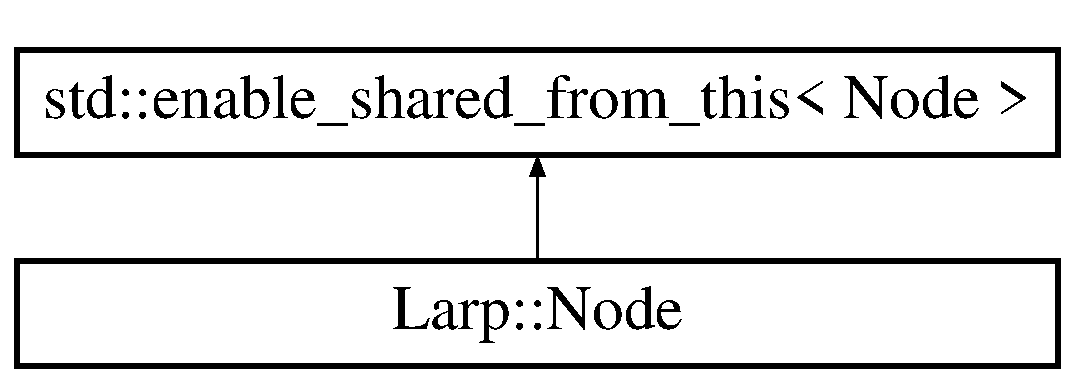
\includegraphics[height=2.000000cm]{classLarp_1_1Node}
\end{center}
\end{figure}
\subsection*{Public Member Functions}
\begin{DoxyCompactItemize}
\item 
\hyperlink{classLarp_1_1Node_a2cb8fc6e60b762b02226d73489ac5099}{Node} ()
\item 
void \hyperlink{classLarp_1_1Node_aa701cc59976ddbd1c232e027df0e4a9b}{draw} (glm\+::mat4 model, glm\+::mat4 \&view, glm\+::mat4 \&projection)
\item 
\hyperlink{namespaceLarp_a57e9a3e29e68cdf508c964274d9ac1a4}{p\+Node} \hyperlink{classLarp_1_1Node_a8dac983fde585084afddddb2ab60c1d8}{create\+\_\+child} ()
\item 
\hyperlink{namespaceLarp_a57e9a3e29e68cdf508c964274d9ac1a4}{p\+Node} \hyperlink{classLarp_1_1Node_a800ecd41070c27d36e7971e55d3b9842}{remove\+\_\+child} (\hyperlink{namespaceLarp_a57e9a3e29e68cdf508c964274d9ac1a4}{p\+Node} \&child)
\item 
void \hyperlink{classLarp_1_1Node_a44070f7bb06cdca4fafbdf65f0d6118e}{set\+\_\+position} (G\+Lfloat x, G\+Lfloat y, G\+Lfloat z)
\item 
void \hyperlink{classLarp_1_1Node_a8eef7a9829817bfe9b2ff3bed5b0c3a8}{set\+\_\+position} (glm\+::vec3 position)
\item 
void \hyperlink{classLarp_1_1Node_ad1b12b56ba7c708d1ce51ec0762f7476}{set\+\_\+orientation} (G\+Lfloat x, G\+Lfloat y, G\+Lfloat z, G\+Lfloat w)
\item 
void \hyperlink{classLarp_1_1Node_a3695bdfa48908be007d751e9c05bdb0e}{set\+\_\+orientation} (glm\+::quat rotation)
\item 
void \hyperlink{classLarp_1_1Node_a0d5e761af674c2c547e8638b91a2a85b}{set\+\_\+orientation} (glm\+::vec3 axis, G\+Lfloat w)
\item 
void \hyperlink{classLarp_1_1Node_a829a3cf29a5f165f7d771cc283f25053}{yaw} (G\+Lfloat yaw)
\item 
void \hyperlink{classLarp_1_1Node_ad8f8390e764a96398d080538c437c7ee}{pitch} (G\+Lfloat pitch)
\item 
void \hyperlink{classLarp_1_1Node_a1c839a3075f1e97aa368ba8212c50ee7}{roll} (G\+Lfloat roll)
\item 
void \hyperlink{classLarp_1_1Node_aa0186c5d77b58e2d7ede02dec0f2cdc4}{translate} (G\+Lfloat x, G\+Lfloat y, G\+Lfloat z)
\item 
void \hyperlink{classLarp_1_1Node_a7494be4e04c8f5911aedeeb41c27993b}{translate} (glm\+::vec3 vec)
\item 
void \hyperlink{classLarp_1_1Node_a20048e6f1487b9e6bdb5e2f66794de65}{set\+\_\+scale} (glm\+::vec3 scale)
\item 
void \hyperlink{classLarp_1_1Node_aa212fa28bc6cc6df4ded2a487fd591eb}{set\+\_\+scale} (G\+Lfloat x, G\+Lfloat y, G\+Lfloat z)
\item 
void \hyperlink{classLarp_1_1Node_a370b5663332a8c802bebedccc1302eac}{attach\+\_\+entity} (\hyperlink{namespaceLarp_aca47662468377e5aaf9a665699a4d97f}{p\+Entity} \&entity)
\item 
\hyperlink{namespaceLarp_aca47662468377e5aaf9a665699a4d97f}{p\+Entity} \hyperlink{classLarp_1_1Node_a21823582d4d4fbe9e1b4414efcba6250}{remove\+\_\+entity} ()
\end{DoxyCompactItemize}
\subsection*{Private Attributes}
\begin{DoxyCompactItemize}
\item 
\hyperlink{namespaceLarp_aca47662468377e5aaf9a665699a4d97f}{p\+Entity} \hyperlink{classLarp_1_1Node_acf7b5cdde90be913d7cf3c226758fc32}{\+\_\+entity}
\item 
std\+::weak\+\_\+ptr$<$ \hyperlink{classLarp_1_1Node}{Node} $>$ \hyperlink{classLarp_1_1Node_a416307326769655e02fbb0b231307711}{\+\_\+parent}
\item 
std\+::unordered\+\_\+set$<$ \hyperlink{namespaceLarp_a57e9a3e29e68cdf508c964274d9ac1a4}{p\+Node} $>$ \hyperlink{classLarp_1_1Node_a006d3873814e2f7243d6457225e0d0fc}{\+\_\+children}
\item 
glm\+::vec3 \hyperlink{classLarp_1_1Node_a060f49eb175b70c9e0da515fa685f1f2}{\+\_\+position}
\item 
glm\+::quat \hyperlink{classLarp_1_1Node_a3bf60bf55c2cda89031f9327fafa0d17}{\+\_\+rotation}
\item 
glm\+::vec3 \hyperlink{classLarp_1_1Node_ae295b7db9065cd5bcc1edb32af6e7987}{\+\_\+scale}
\end{DoxyCompactItemize}


\subsection{Constructor \& Destructor Documentation}
\index{Larp\+::\+Node@{Larp\+::\+Node}!Node@{Node}}
\index{Node@{Node}!Larp\+::\+Node@{Larp\+::\+Node}}
\subsubsection[{\texorpdfstring{Node()}{Node()}}]{\setlength{\rightskip}{0pt plus 5cm}Larp\+::\+Node\+::\+Node (
\begin{DoxyParamCaption}
{}
\end{DoxyParamCaption}
)}\hypertarget{classLarp_1_1Node_a2cb8fc6e60b762b02226d73489ac5099}{}\label{classLarp_1_1Node_a2cb8fc6e60b762b02226d73489ac5099}
Default Constructor Initializes the \hyperlink{classLarp_1_1Node}{Node} to be at the parent\textquotesingle{}s origin, unrotated relative to the parent, and to have the same scale as the parent 

\subsection{Member Function Documentation}
\index{Larp\+::\+Node@{Larp\+::\+Node}!attach\+\_\+entity@{attach\+\_\+entity}}
\index{attach\+\_\+entity@{attach\+\_\+entity}!Larp\+::\+Node@{Larp\+::\+Node}}
\subsubsection[{\texorpdfstring{attach\+\_\+entity(p\+Entity \&entity)}{attach_entity(pEntity &entity)}}]{\setlength{\rightskip}{0pt plus 5cm}void Larp\+::\+Node\+::attach\+\_\+entity (
\begin{DoxyParamCaption}
\item[{{\bf p\+Entity} \&}]{entity}
\end{DoxyParamCaption}
)}\hypertarget{classLarp_1_1Node_a370b5663332a8c802bebedccc1302eac}{}\label{classLarp_1_1Node_a370b5663332a8c802bebedccc1302eac}
Attaches a p\+Entity to this object 
\begin{DoxyParams}{Parameters}
{\em entity} & The p\+Entity to attach to this object \\
\hline
\end{DoxyParams}
\index{Larp\+::\+Node@{Larp\+::\+Node}!create\+\_\+child@{create\+\_\+child}}
\index{create\+\_\+child@{create\+\_\+child}!Larp\+::\+Node@{Larp\+::\+Node}}
\subsubsection[{\texorpdfstring{create\+\_\+child()}{create_child()}}]{\setlength{\rightskip}{0pt plus 5cm}{\bf p\+Node} Larp\+::\+Node\+::create\+\_\+child (
\begin{DoxyParamCaption}
{}
\end{DoxyParamCaption}
)}\hypertarget{classLarp_1_1Node_a8dac983fde585084afddddb2ab60c1d8}{}\label{classLarp_1_1Node_a8dac983fde585084afddddb2ab60c1d8}
Creates a new \hyperlink{classLarp_1_1Node}{Node} that is a child of this \hyperlink{classLarp_1_1Node}{Node}. \begin{DoxyReturn}{Returns}
A pointer to the new \hyperlink{classLarp_1_1Node}{Node} 
\end{DoxyReturn}
\index{Larp\+::\+Node@{Larp\+::\+Node}!draw@{draw}}
\index{draw@{draw}!Larp\+::\+Node@{Larp\+::\+Node}}
\subsubsection[{\texorpdfstring{draw(glm\+::mat4 model, glm\+::mat4 \&view, glm\+::mat4 \&projection)}{draw(glm::mat4 model, glm::mat4 &view, glm::mat4 &projection)}}]{\setlength{\rightskip}{0pt plus 5cm}void Larp\+::\+Node\+::draw (
\begin{DoxyParamCaption}
\item[{glm\+::mat4}]{model, }
\item[{glm\+::mat4 \&}]{view, }
\item[{glm\+::mat4 \&}]{projection}
\end{DoxyParamCaption}
)}\hypertarget{classLarp_1_1Node_aa701cc59976ddbd1c232e027df0e4a9b}{}\label{classLarp_1_1Node_aa701cc59976ddbd1c232e027df0e4a9b}
Draws the \hyperlink{classLarp_1_1Entity}{Entity} attached to this node using this \hyperlink{classLarp_1_1Node}{Node}\textquotesingle{}s derived model matrix, then recursively calls the draw method on each of this \hyperlink{classLarp_1_1Node}{Node}\textquotesingle{}s children. \begin{DoxyNote}{Note}
the order in which the draw method is called on the \hyperlink{classLarp_1_1Node}{Node}\textquotesingle{}s children is not necessarily the order in which they were created. 
\end{DoxyNote}
\index{Larp\+::\+Node@{Larp\+::\+Node}!pitch@{pitch}}
\index{pitch@{pitch}!Larp\+::\+Node@{Larp\+::\+Node}}
\subsubsection[{\texorpdfstring{pitch(\+G\+Lfloat pitch)}{pitch(GLfloat pitch)}}]{\setlength{\rightskip}{0pt plus 5cm}void Larp\+::\+Node\+::pitch (
\begin{DoxyParamCaption}
\item[{G\+Lfloat}]{pitch}
\end{DoxyParamCaption}
)}\hypertarget{classLarp_1_1Node_ad8f8390e764a96398d080538c437c7ee}{}\label{classLarp_1_1Node_ad8f8390e764a96398d080538c437c7ee}
Pitchs the \hyperlink{classLarp_1_1Node}{Node} 
\begin{DoxyParams}{Parameters}
{\em pitch} & The degrees to pitch this \hyperlink{classLarp_1_1Node}{Node} \\
\hline
\end{DoxyParams}
\begin{DoxyNote}{Note}
This function expects pitch in degrees 

This function adds to any pitch amount already applied to the \hyperlink{classLarp_1_1Node}{Node} 
\end{DoxyNote}
\index{Larp\+::\+Node@{Larp\+::\+Node}!remove\+\_\+child@{remove\+\_\+child}}
\index{remove\+\_\+child@{remove\+\_\+child}!Larp\+::\+Node@{Larp\+::\+Node}}
\subsubsection[{\texorpdfstring{remove\+\_\+child(p\+Node \&child)}{remove_child(pNode &child)}}]{\setlength{\rightskip}{0pt plus 5cm}{\bf p\+Node} Larp\+::\+Node\+::remove\+\_\+child (
\begin{DoxyParamCaption}
\item[{{\bf p\+Node} \&}]{child}
\end{DoxyParamCaption}
)}\hypertarget{classLarp_1_1Node_a800ecd41070c27d36e7971e55d3b9842}{}\label{classLarp_1_1Node_a800ecd41070c27d36e7971e55d3b9842}
Removes a given p\+Node as a child of this \hyperlink{classLarp_1_1Node}{Node} object. \begin{DoxyReturn}{Returns}
the p\+Node that was removed 
\end{DoxyReturn}
\index{Larp\+::\+Node@{Larp\+::\+Node}!remove\+\_\+entity@{remove\+\_\+entity}}
\index{remove\+\_\+entity@{remove\+\_\+entity}!Larp\+::\+Node@{Larp\+::\+Node}}
\subsubsection[{\texorpdfstring{remove\+\_\+entity()}{remove_entity()}}]{\setlength{\rightskip}{0pt plus 5cm}{\bf p\+Entity} Larp\+::\+Node\+::remove\+\_\+entity (
\begin{DoxyParamCaption}
{}
\end{DoxyParamCaption}
)}\hypertarget{classLarp_1_1Node_a21823582d4d4fbe9e1b4414efcba6250}{}\label{classLarp_1_1Node_a21823582d4d4fbe9e1b4414efcba6250}
Detaches the p\+Entity from this \hyperlink{classLarp_1_1Node}{Node} \begin{DoxyReturn}{Returns}
the p\+Entity that was removed from this \hyperlink{classLarp_1_1Node}{Node} 
\end{DoxyReturn}
\index{Larp\+::\+Node@{Larp\+::\+Node}!roll@{roll}}
\index{roll@{roll}!Larp\+::\+Node@{Larp\+::\+Node}}
\subsubsection[{\texorpdfstring{roll(\+G\+Lfloat roll)}{roll(GLfloat roll)}}]{\setlength{\rightskip}{0pt plus 5cm}void Larp\+::\+Node\+::roll (
\begin{DoxyParamCaption}
\item[{G\+Lfloat}]{roll}
\end{DoxyParamCaption}
)}\hypertarget{classLarp_1_1Node_a1c839a3075f1e97aa368ba8212c50ee7}{}\label{classLarp_1_1Node_a1c839a3075f1e97aa368ba8212c50ee7}
Rolls the \hyperlink{classLarp_1_1Node}{Node} 
\begin{DoxyParams}{Parameters}
{\em roll} & The degrees to roll this \hyperlink{classLarp_1_1Node}{Node} \\
\hline
\end{DoxyParams}
\begin{DoxyNote}{Note}
This function expects roll in degrees 

This function adds to any roll amount already applied to the \hyperlink{classLarp_1_1Node}{Node} 
\end{DoxyNote}
\index{Larp\+::\+Node@{Larp\+::\+Node}!set\+\_\+orientation@{set\+\_\+orientation}}
\index{set\+\_\+orientation@{set\+\_\+orientation}!Larp\+::\+Node@{Larp\+::\+Node}}
\subsubsection[{\texorpdfstring{set\+\_\+orientation(\+G\+Lfloat x, G\+Lfloat y, G\+Lfloat z, G\+Lfloat w)}{set_orientation(GLfloat x, GLfloat y, GLfloat z, GLfloat w)}}]{\setlength{\rightskip}{0pt plus 5cm}void Larp\+::\+Node\+::set\+\_\+orientation (
\begin{DoxyParamCaption}
\item[{G\+Lfloat}]{x, }
\item[{G\+Lfloat}]{y, }
\item[{G\+Lfloat}]{z, }
\item[{G\+Lfloat}]{w}
\end{DoxyParamCaption}
)}\hypertarget{classLarp_1_1Node_ad1b12b56ba7c708d1ce51ec0762f7476}{}\label{classLarp_1_1Node_ad1b12b56ba7c708d1ce51ec0762f7476}
Sets the orientation of this \hyperlink{classLarp_1_1Node}{Node} 
\begin{DoxyParams}{Parameters}
{\em x} & The x-\/direction of the axis of rotation \\
\hline
{\em y} & The y-\/direction of the axis of rotation \\
\hline
{\em z} & The z-\/direction of the axis of rotation \\
\hline
{\em w} & The angular component of the rotation, in degrees \\
\hline
\end{DoxyParams}
\begin{DoxyNote}{Note}
This function expects w in degrees 
\end{DoxyNote}
\begin{DoxyWarning}{Warning}
This function expects an expanded version of the (axis, angle) quaternion representation, {\bfseries not} the same 4-\/components that glm\+::quat(w, x, y, z) expect. 
\end{DoxyWarning}
\index{Larp\+::\+Node@{Larp\+::\+Node}!set\+\_\+orientation@{set\+\_\+orientation}}
\index{set\+\_\+orientation@{set\+\_\+orientation}!Larp\+::\+Node@{Larp\+::\+Node}}
\subsubsection[{\texorpdfstring{set\+\_\+orientation(glm\+::quat rotation)}{set_orientation(glm::quat rotation)}}]{\setlength{\rightskip}{0pt plus 5cm}void Larp\+::\+Node\+::set\+\_\+orientation (
\begin{DoxyParamCaption}
\item[{glm\+::quat}]{rotation}
\end{DoxyParamCaption}
)}\hypertarget{classLarp_1_1Node_a3695bdfa48908be007d751e9c05bdb0e}{}\label{classLarp_1_1Node_a3695bdfa48908be007d751e9c05bdb0e}
Sets the orientation of this \hyperlink{classLarp_1_1Node}{Node} 
\begin{DoxyParams}{Parameters}
{\em rotation} & The amount to rotate this \hyperlink{classLarp_1_1Node}{Node} \\
\hline
\end{DoxyParams}
\begin{DoxyWarning}{Warning}
This function expects a properly computed glm\+::quat, such as one obtained by calling glm\+::angle\+Axis(). 
\end{DoxyWarning}
\index{Larp\+::\+Node@{Larp\+::\+Node}!set\+\_\+orientation@{set\+\_\+orientation}}
\index{set\+\_\+orientation@{set\+\_\+orientation}!Larp\+::\+Node@{Larp\+::\+Node}}
\subsubsection[{\texorpdfstring{set\+\_\+orientation(glm\+::vec3 axis, G\+Lfloat w)}{set_orientation(glm::vec3 axis, GLfloat w)}}]{\setlength{\rightskip}{0pt plus 5cm}void Larp\+::\+Node\+::set\+\_\+orientation (
\begin{DoxyParamCaption}
\item[{glm\+::vec3}]{axis, }
\item[{G\+Lfloat}]{w}
\end{DoxyParamCaption}
)}\hypertarget{classLarp_1_1Node_a0d5e761af674c2c547e8638b91a2a85b}{}\label{classLarp_1_1Node_a0d5e761af674c2c547e8638b91a2a85b}
Sets the orientation of this \hyperlink{classLarp_1_1Node}{Node} 
\begin{DoxyParams}{Parameters}
{\em axis} & The axis of rotation \\
\hline
{\em w} & The angle of rotation, in degrees \\
\hline
\end{DoxyParams}
\begin{DoxyNote}{Note}
This function expects w in degrees 
\end{DoxyNote}
\index{Larp\+::\+Node@{Larp\+::\+Node}!set\+\_\+position@{set\+\_\+position}}
\index{set\+\_\+position@{set\+\_\+position}!Larp\+::\+Node@{Larp\+::\+Node}}
\subsubsection[{\texorpdfstring{set\+\_\+position(\+G\+Lfloat x, G\+Lfloat y, G\+Lfloat z)}{set_position(GLfloat x, GLfloat y, GLfloat z)}}]{\setlength{\rightskip}{0pt plus 5cm}void Larp\+::\+Node\+::set\+\_\+position (
\begin{DoxyParamCaption}
\item[{G\+Lfloat}]{x, }
\item[{G\+Lfloat}]{y, }
\item[{G\+Lfloat}]{z}
\end{DoxyParamCaption}
)}\hypertarget{classLarp_1_1Node_a44070f7bb06cdca4fafbdf65f0d6118e}{}\label{classLarp_1_1Node_a44070f7bb06cdca4fafbdf65f0d6118e}
Sets the position of this \hyperlink{classLarp_1_1Node}{Node} 
\begin{DoxyParams}{Parameters}
{\em x} & The new x position. \\
\hline
{\em y} & The new y position. \\
\hline
{\em z} & The new z position. \\
\hline
\end{DoxyParams}
\index{Larp\+::\+Node@{Larp\+::\+Node}!set\+\_\+position@{set\+\_\+position}}
\index{set\+\_\+position@{set\+\_\+position}!Larp\+::\+Node@{Larp\+::\+Node}}
\subsubsection[{\texorpdfstring{set\+\_\+position(glm\+::vec3 position)}{set_position(glm::vec3 position)}}]{\setlength{\rightskip}{0pt plus 5cm}void Larp\+::\+Node\+::set\+\_\+position (
\begin{DoxyParamCaption}
\item[{glm\+::vec3}]{position}
\end{DoxyParamCaption}
)}\hypertarget{classLarp_1_1Node_a8eef7a9829817bfe9b2ff3bed5b0c3a8}{}\label{classLarp_1_1Node_a8eef7a9829817bfe9b2ff3bed5b0c3a8}
Sets the position of this \hyperlink{classLarp_1_1Node}{Node} 
\begin{DoxyParams}{Parameters}
{\em position} & The new position of this \hyperlink{classLarp_1_1Node}{Node} \\
\hline
\end{DoxyParams}
\index{Larp\+::\+Node@{Larp\+::\+Node}!set\+\_\+scale@{set\+\_\+scale}}
\index{set\+\_\+scale@{set\+\_\+scale}!Larp\+::\+Node@{Larp\+::\+Node}}
\subsubsection[{\texorpdfstring{set\+\_\+scale(glm\+::vec3 scale)}{set_scale(glm::vec3 scale)}}]{\setlength{\rightskip}{0pt plus 5cm}void Larp\+::\+Node\+::set\+\_\+scale (
\begin{DoxyParamCaption}
\item[{glm\+::vec3}]{scale}
\end{DoxyParamCaption}
)}\hypertarget{classLarp_1_1Node_a20048e6f1487b9e6bdb5e2f66794de65}{}\label{classLarp_1_1Node_a20048e6f1487b9e6bdb5e2f66794de65}
Scales the \hyperlink{classLarp_1_1Node}{Node} 
\begin{DoxyParams}{Parameters}
{\em scale} & The number of units to scale this \hyperlink{classLarp_1_1Node}{Node} in the x-\/, y-\/, and z-\/directions \\
\hline
\end{DoxyParams}
\index{Larp\+::\+Node@{Larp\+::\+Node}!set\+\_\+scale@{set\+\_\+scale}}
\index{set\+\_\+scale@{set\+\_\+scale}!Larp\+::\+Node@{Larp\+::\+Node}}
\subsubsection[{\texorpdfstring{set\+\_\+scale(\+G\+Lfloat x, G\+Lfloat y, G\+Lfloat z)}{set_scale(GLfloat x, GLfloat y, GLfloat z)}}]{\setlength{\rightskip}{0pt plus 5cm}void Larp\+::\+Node\+::set\+\_\+scale (
\begin{DoxyParamCaption}
\item[{G\+Lfloat}]{x, }
\item[{G\+Lfloat}]{y, }
\item[{G\+Lfloat}]{z}
\end{DoxyParamCaption}
)}\hypertarget{classLarp_1_1Node_aa212fa28bc6cc6df4ded2a487fd591eb}{}\label{classLarp_1_1Node_aa212fa28bc6cc6df4ded2a487fd591eb}
Scales the \hyperlink{classLarp_1_1Node}{Node} 
\begin{DoxyParams}{Parameters}
{\em x} & The number of units to scale this \hyperlink{classLarp_1_1Node}{Node} in the x-\/direction \\
\hline
{\em y} & The number of units to scale this \hyperlink{classLarp_1_1Node}{Node} in the y-\/direction \\
\hline
{\em z} & The number of units to scale this \hyperlink{classLarp_1_1Node}{Node} in the z-\/direction \\
\hline
\end{DoxyParams}
\index{Larp\+::\+Node@{Larp\+::\+Node}!translate@{translate}}
\index{translate@{translate}!Larp\+::\+Node@{Larp\+::\+Node}}
\subsubsection[{\texorpdfstring{translate(\+G\+Lfloat x, G\+Lfloat y, G\+Lfloat z)}{translate(GLfloat x, GLfloat y, GLfloat z)}}]{\setlength{\rightskip}{0pt plus 5cm}void Larp\+::\+Node\+::translate (
\begin{DoxyParamCaption}
\item[{G\+Lfloat}]{x, }
\item[{G\+Lfloat}]{y, }
\item[{G\+Lfloat}]{z}
\end{DoxyParamCaption}
)}\hypertarget{classLarp_1_1Node_aa0186c5d77b58e2d7ede02dec0f2cdc4}{}\label{classLarp_1_1Node_aa0186c5d77b58e2d7ede02dec0f2cdc4}
Translates the \hyperlink{classLarp_1_1Node}{Node} 
\begin{DoxyParams}{Parameters}
{\em x} & The number of units in the x-\/direction to translate this \hyperlink{classLarp_1_1Node}{Node} \\
\hline
{\em y} & The number of units in the y-\/direction to translate this \hyperlink{classLarp_1_1Node}{Node} \\
\hline
{\em z} & The number of units in the z-\/direction to translate this \hyperlink{classLarp_1_1Node}{Node} \\
\hline
\end{DoxyParams}
\begin{DoxyNote}{Note}
This function adds to any translation amount already applied to the \hyperlink{classLarp_1_1Node}{Node} 
\end{DoxyNote}
\index{Larp\+::\+Node@{Larp\+::\+Node}!translate@{translate}}
\index{translate@{translate}!Larp\+::\+Node@{Larp\+::\+Node}}
\subsubsection[{\texorpdfstring{translate(glm\+::vec3 vec)}{translate(glm::vec3 vec)}}]{\setlength{\rightskip}{0pt plus 5cm}void Larp\+::\+Node\+::translate (
\begin{DoxyParamCaption}
\item[{glm\+::vec3}]{vec}
\end{DoxyParamCaption}
)}\hypertarget{classLarp_1_1Node_a7494be4e04c8f5911aedeeb41c27993b}{}\label{classLarp_1_1Node_a7494be4e04c8f5911aedeeb41c27993b}
Translates the \hyperlink{classLarp_1_1Node}{Node} 
\begin{DoxyParams}{Parameters}
{\em vec} & The number of units to translate this \hyperlink{classLarp_1_1Node}{Node} in the x-\/, y-\/, and z-\/directions \\
\hline
\end{DoxyParams}
\begin{DoxyNote}{Note}
This function adds to any translation amount already applied to the \hyperlink{classLarp_1_1Node}{Node} 
\end{DoxyNote}
\index{Larp\+::\+Node@{Larp\+::\+Node}!yaw@{yaw}}
\index{yaw@{yaw}!Larp\+::\+Node@{Larp\+::\+Node}}
\subsubsection[{\texorpdfstring{yaw(\+G\+Lfloat yaw)}{yaw(GLfloat yaw)}}]{\setlength{\rightskip}{0pt plus 5cm}void Larp\+::\+Node\+::yaw (
\begin{DoxyParamCaption}
\item[{G\+Lfloat}]{yaw}
\end{DoxyParamCaption}
)}\hypertarget{classLarp_1_1Node_a829a3cf29a5f165f7d771cc283f25053}{}\label{classLarp_1_1Node_a829a3cf29a5f165f7d771cc283f25053}
Yaws the \hyperlink{classLarp_1_1Node}{Node} 
\begin{DoxyParams}{Parameters}
{\em yaw} & The degrees to yaw this \hyperlink{classLarp_1_1Node}{Node} \\
\hline
\end{DoxyParams}
\begin{DoxyNote}{Note}
This function expects yaw in degrees 

This function adds to any yaw amount already applied to the \hyperlink{classLarp_1_1Node}{Node} 
\end{DoxyNote}


\subsection{Member Data Documentation}
\index{Larp\+::\+Node@{Larp\+::\+Node}!\+\_\+children@{\+\_\+children}}
\index{\+\_\+children@{\+\_\+children}!Larp\+::\+Node@{Larp\+::\+Node}}
\subsubsection[{\texorpdfstring{\+\_\+children}{_children}}]{\setlength{\rightskip}{0pt plus 5cm}std\+::unordered\+\_\+set$<${\bf p\+Node}$>$ Larp\+::\+Node\+::\+\_\+children\hspace{0.3cm}{\ttfamily [private]}}\hypertarget{classLarp_1_1Node_a006d3873814e2f7243d6457225e0d0fc}{}\label{classLarp_1_1Node_a006d3873814e2f7243d6457225e0d0fc}
All of this \hyperlink{classLarp_1_1Node}{Node}\textquotesingle{}s child \hyperlink{classLarp_1_1Node}{Node}\textquotesingle{}s \index{Larp\+::\+Node@{Larp\+::\+Node}!\+\_\+entity@{\+\_\+entity}}
\index{\+\_\+entity@{\+\_\+entity}!Larp\+::\+Node@{Larp\+::\+Node}}
\subsubsection[{\texorpdfstring{\+\_\+entity}{_entity}}]{\setlength{\rightskip}{0pt plus 5cm}{\bf p\+Entity} Larp\+::\+Node\+::\+\_\+entity\hspace{0.3cm}{\ttfamily [private]}}\hypertarget{classLarp_1_1Node_acf7b5cdde90be913d7cf3c226758fc32}{}\label{classLarp_1_1Node_acf7b5cdde90be913d7cf3c226758fc32}
The \hyperlink{classLarp_1_1Entity}{Entity} object attached to this \hyperlink{classLarp_1_1Node}{Node}. Drawn during rendering. \index{Larp\+::\+Node@{Larp\+::\+Node}!\+\_\+parent@{\+\_\+parent}}
\index{\+\_\+parent@{\+\_\+parent}!Larp\+::\+Node@{Larp\+::\+Node}}
\subsubsection[{\texorpdfstring{\+\_\+parent}{_parent}}]{\setlength{\rightskip}{0pt plus 5cm}std\+::weak\+\_\+ptr$<${\bf Node}$>$ Larp\+::\+Node\+::\+\_\+parent\hspace{0.3cm}{\ttfamily [private]}}\hypertarget{classLarp_1_1Node_a416307326769655e02fbb0b231307711}{}\label{classLarp_1_1Node_a416307326769655e02fbb0b231307711}
This \hyperlink{classLarp_1_1Node}{Node}\textquotesingle{}s parent \hyperlink{classLarp_1_1Node}{Node}. \index{Larp\+::\+Node@{Larp\+::\+Node}!\+\_\+position@{\+\_\+position}}
\index{\+\_\+position@{\+\_\+position}!Larp\+::\+Node@{Larp\+::\+Node}}
\subsubsection[{\texorpdfstring{\+\_\+position}{_position}}]{\setlength{\rightskip}{0pt plus 5cm}glm\+::vec3 Larp\+::\+Node\+::\+\_\+position\hspace{0.3cm}{\ttfamily [private]}}\hypertarget{classLarp_1_1Node_a060f49eb175b70c9e0da515fa685f1f2}{}\label{classLarp_1_1Node_a060f49eb175b70c9e0da515fa685f1f2}
This \hyperlink{classLarp_1_1Node}{Node}\textquotesingle{}s position \index{Larp\+::\+Node@{Larp\+::\+Node}!\+\_\+rotation@{\+\_\+rotation}}
\index{\+\_\+rotation@{\+\_\+rotation}!Larp\+::\+Node@{Larp\+::\+Node}}
\subsubsection[{\texorpdfstring{\+\_\+rotation}{_rotation}}]{\setlength{\rightskip}{0pt plus 5cm}glm\+::quat Larp\+::\+Node\+::\+\_\+rotation\hspace{0.3cm}{\ttfamily [private]}}\hypertarget{classLarp_1_1Node_a3bf60bf55c2cda89031f9327fafa0d17}{}\label{classLarp_1_1Node_a3bf60bf55c2cda89031f9327fafa0d17}
This \hyperlink{classLarp_1_1Node}{Node}\textquotesingle{}s rotation \index{Larp\+::\+Node@{Larp\+::\+Node}!\+\_\+scale@{\+\_\+scale}}
\index{\+\_\+scale@{\+\_\+scale}!Larp\+::\+Node@{Larp\+::\+Node}}
\subsubsection[{\texorpdfstring{\+\_\+scale}{_scale}}]{\setlength{\rightskip}{0pt plus 5cm}glm\+::vec3 Larp\+::\+Node\+::\+\_\+scale\hspace{0.3cm}{\ttfamily [private]}}\hypertarget{classLarp_1_1Node_ae295b7db9065cd5bcc1edb32af6e7987}{}\label{classLarp_1_1Node_ae295b7db9065cd5bcc1edb32af6e7987}
This \hyperlink{classLarp_1_1Node}{Node}\textquotesingle{}s scale 

The documentation for this class was generated from the following files\+:\begin{DoxyCompactItemize}
\item 
src/\hyperlink{Node_8hpp}{Node.\+hpp}\item 
src/\hyperlink{Node_8cpp}{Node.\+cpp}\end{DoxyCompactItemize}

\hypertarget{classPhysicsMeshCollider}{}\section{Physics\+Mesh\+Collider Class Reference}
\label{classPhysicsMeshCollider}\index{Physics\+Mesh\+Collider@{Physics\+Mesh\+Collider}}


{\ttfamily \#include $<$Physics\+Mesh\+Collider.\+hpp$>$}

\subsection*{Public Member Functions}
\begin{DoxyCompactItemize}
\item 
\hyperlink{classPhysicsMeshCollider_a01693b5b41b6bce02cab01cab3ebb9d5}{Physics\+Mesh\+Collider} (\hyperlink{namespaceLarp_a1fbc1dec59f7a571dc06e152b1e7d38c}{Larp\+::\+Model\+Ptr} model, glm\+::quat rotation, glm\+::vec3 position, G\+Lfloat mass, glm\+::vec3 local\+\_\+inertia, G\+Lfloat restitution, \hyperlink{namespaceLarp_a171c1dc8b70cfb441b15d7386780db23}{Larp\+::\+Node\+Ptr} user\+\_\+pointer)
\item 
bt\+Rigid\+Body $\ast$ \hyperlink{classPhysicsMeshCollider_a2518cb2798d507046a1f8e356f8a6f56}{get\+\_\+rigid\+\_\+body} () const 
\end{DoxyCompactItemize}
\subsection*{Private Attributes}
\begin{DoxyCompactItemize}
\item 
bt\+Rigid\+Body $\ast$ \hyperlink{classPhysicsMeshCollider_a79bf728a386ac89b63c4ded82af6762b}{\+\_\+rigid\+\_\+body}
\end{DoxyCompactItemize}


\subsection{Constructor \& Destructor Documentation}
\index{Physics\+Mesh\+Collider@{Physics\+Mesh\+Collider}!Physics\+Mesh\+Collider@{Physics\+Mesh\+Collider}}
\index{Physics\+Mesh\+Collider@{Physics\+Mesh\+Collider}!Physics\+Mesh\+Collider@{Physics\+Mesh\+Collider}}
\subsubsection[{\texorpdfstring{Physics\+Mesh\+Collider(\+Larp\+::\+Model\+Ptr model, glm\+::quat rotation, glm\+::vec3 position, G\+Lfloat mass, glm\+::vec3 local\+\_\+inertia, G\+Lfloat restitution, Larp\+::\+Node\+Ptr user\+\_\+pointer)}{PhysicsMeshCollider(Larp::ModelPtr model, glm::quat rotation, glm::vec3 position, GLfloat mass, glm::vec3 local_inertia, GLfloat restitution, Larp::NodePtr user_pointer)}}]{\setlength{\rightskip}{0pt plus 5cm}Physics\+Mesh\+Collider\+::\+Physics\+Mesh\+Collider (
\begin{DoxyParamCaption}
\item[{{\bf Larp\+::\+Model\+Ptr}}]{model, }
\item[{glm\+::quat}]{rotation, }
\item[{glm\+::vec3}]{position, }
\item[{G\+Lfloat}]{mass, }
\item[{glm\+::vec3}]{local\+\_\+inertia, }
\item[{G\+Lfloat}]{restitution, }
\item[{{\bf Larp\+::\+Node\+Ptr}}]{user\+\_\+pointer}
\end{DoxyParamCaption}
)}\hypertarget{classPhysicsMeshCollider_a01693b5b41b6bce02cab01cab3ebb9d5}{}\label{classPhysicsMeshCollider_a01693b5b41b6bce02cab01cab3ebb9d5}
For each mesh in the model, we need to grab each face in that mesh. The faces are defined in mesh.\+\_\+indices, which has a face defined for every 3 indices, and each of the indices point to a Vertex in mesh.\+\_\+vertices

\subsection{Member Function Documentation}
\index{Physics\+Mesh\+Collider@{Physics\+Mesh\+Collider}!get\+\_\+rigid\+\_\+body@{get\+\_\+rigid\+\_\+body}}
\index{get\+\_\+rigid\+\_\+body@{get\+\_\+rigid\+\_\+body}!Physics\+Mesh\+Collider@{Physics\+Mesh\+Collider}}
\subsubsection[{\texorpdfstring{get\+\_\+rigid\+\_\+body() const }{get_rigid_body() const }}]{\setlength{\rightskip}{0pt plus 5cm}bt\+Rigid\+Body $\ast$ Physics\+Mesh\+Collider\+::get\+\_\+rigid\+\_\+body (
\begin{DoxyParamCaption}
{}
\end{DoxyParamCaption}
) const}\hypertarget{classPhysicsMeshCollider_a2518cb2798d507046a1f8e356f8a6f56}{}\label{classPhysicsMeshCollider_a2518cb2798d507046a1f8e356f8a6f56}


\subsection{Member Data Documentation}
\index{Physics\+Mesh\+Collider@{Physics\+Mesh\+Collider}!\+\_\+rigid\+\_\+body@{\+\_\+rigid\+\_\+body}}
\index{\+\_\+rigid\+\_\+body@{\+\_\+rigid\+\_\+body}!Physics\+Mesh\+Collider@{Physics\+Mesh\+Collider}}
\subsubsection[{\texorpdfstring{\+\_\+rigid\+\_\+body}{_rigid_body}}]{\setlength{\rightskip}{0pt plus 5cm}bt\+Rigid\+Body$\ast$ Physics\+Mesh\+Collider\+::\+\_\+rigid\+\_\+body\hspace{0.3cm}{\ttfamily [private]}}\hypertarget{classPhysicsMeshCollider_a79bf728a386ac89b63c4ded82af6762b}{}\label{classPhysicsMeshCollider_a79bf728a386ac89b63c4ded82af6762b}


The documentation for this class was generated from the following files\+:\begin{DoxyCompactItemize}
\item 
src/\+Physics/\hyperlink{PhysicsMeshCollider_8hpp}{Physics\+Mesh\+Collider.\+hpp}\item 
src/\+Physics/\hyperlink{PhysicsMeshCollider_8cpp}{Physics\+Mesh\+Collider.\+cpp}\end{DoxyCompactItemize}

\hypertarget{classPhysicsMeshColliderBuilder}{}\section{Physics\+Mesh\+Collider\+Builder Class Reference}
\label{classPhysicsMeshColliderBuilder}\index{Physics\+Mesh\+Collider\+Builder@{Physics\+Mesh\+Collider\+Builder}}


{\ttfamily \#include $<$Physics\+Mesh\+Collider\+Builder.\+hpp$>$}

\subsection*{Public Member Functions}
\begin{DoxyCompactItemize}
\item 
\hyperlink{classPhysicsMeshColliderBuilder_a952bf520c1027f8e0eb5578a5cd25b89}{Physics\+Mesh\+Collider\+Builder} (std\+::string path)
\item 
void \hyperlink{classPhysicsMeshColliderBuilder_a7d0c5bfaf8e0bca011ee311ed4c36fc9}{set\+\_\+orientation} (glm\+::quat orientation)
\item 
void \hyperlink{classPhysicsMeshColliderBuilder_aaf6db772b22a11411492b3f43fc95f88}{set\+\_\+position} (glm\+::vec3 position)
\item 
void \hyperlink{classPhysicsMeshColliderBuilder_a011838ad8805502d286182e8017fe3a7}{set\+\_\+mass} (G\+Lfloat mass)
\item 
void \hyperlink{classPhysicsMeshColliderBuilder_a37138f70dbc02843fa06a661f8624439}{set\+\_\+local\+\_\+inertia} (glm\+::vec3 local\+\_\+inertia)
\item 
void \hyperlink{classPhysicsMeshColliderBuilder_a8262d206da5afc9aa1f60471a0c37f1c}{set\+\_\+restitution} (G\+Lfloat restitution)
\item 
void \hyperlink{classPhysicsMeshColliderBuilder_a1c85c9d22611d1b78ef867e04b3bcc07}{set\+\_\+user\+\_\+pointer} (\hyperlink{namespaceLarp_a171c1dc8b70cfb441b15d7386780db23}{Larp\+::\+Node\+Ptr} user\+\_\+pointer)
\item 
\hyperlink{PhysicsMeshCollider_8hpp_a60e5aab5f281e1dc60a635fae2466a6e}{Physics\+Mesh\+Collider\+Ptr} \hyperlink{classPhysicsMeshColliderBuilder_a3136483052f4740f1bb544b212f78cc2}{build} ()
\end{DoxyCompactItemize}
\subsection*{Private Attributes}
\begin{DoxyCompactItemize}
\item 
\hyperlink{namespaceLarp_a1fbc1dec59f7a571dc06e152b1e7d38c}{Larp\+::\+Model\+Ptr} \hyperlink{classPhysicsMeshColliderBuilder_a41bb17e3b830ef92b2f04d500a25a829}{\+\_\+model}
\item 
glm\+::quat \hyperlink{classPhysicsMeshColliderBuilder_a443158e70fca5a8df35e90b99e75c6b9}{\+\_\+orientation}
\item 
glm\+::vec3 \hyperlink{classPhysicsMeshColliderBuilder_a1ed543ce75168fc3516a43095f375986}{\+\_\+position}
\item 
G\+Lfloat \hyperlink{classPhysicsMeshColliderBuilder_ab1829c5f0156de48786ea2a2971bb5e0}{\+\_\+mass}
\item 
glm\+::vec3 \hyperlink{classPhysicsMeshColliderBuilder_a5916a7f1e88bb3ac4fc38e1826ba9539}{\+\_\+local\+\_\+inertia}
\item 
G\+Lfloat \hyperlink{classPhysicsMeshColliderBuilder_afd9be67d71afcfedbb4a245e38db0947}{\+\_\+restitution}
\item 
\hyperlink{classLarp_1_1Node}{Larp\+::\+Node} $\ast$ \hyperlink{classPhysicsMeshColliderBuilder_adef014a03eaa91a9006d50267d1068b3}{\+\_\+user\+\_\+pointer}
\end{DoxyCompactItemize}


\subsection{Constructor \& Destructor Documentation}
\index{Physics\+Mesh\+Collider\+Builder@{Physics\+Mesh\+Collider\+Builder}!Physics\+Mesh\+Collider\+Builder@{Physics\+Mesh\+Collider\+Builder}}
\index{Physics\+Mesh\+Collider\+Builder@{Physics\+Mesh\+Collider\+Builder}!Physics\+Mesh\+Collider\+Builder@{Physics\+Mesh\+Collider\+Builder}}
\subsubsection[{\texorpdfstring{Physics\+Mesh\+Collider\+Builder(std\+::string path)}{PhysicsMeshColliderBuilder(std::string path)}}]{\setlength{\rightskip}{0pt plus 5cm}Physics\+Mesh\+Collider\+Builder\+::\+Physics\+Mesh\+Collider\+Builder (
\begin{DoxyParamCaption}
\item[{std\+::string}]{path}
\end{DoxyParamCaption}
)}\hypertarget{classPhysicsMeshColliderBuilder_a952bf520c1027f8e0eb5578a5cd25b89}{}\label{classPhysicsMeshColliderBuilder_a952bf520c1027f8e0eb5578a5cd25b89}
Constructor 
\begin{DoxyParams}{Parameters}
{\em path} & The path to the Model to build a Mesh\+Collider off of \\
\hline
\end{DoxyParams}


\subsection{Member Function Documentation}
\index{Physics\+Mesh\+Collider\+Builder@{Physics\+Mesh\+Collider\+Builder}!build@{build}}
\index{build@{build}!Physics\+Mesh\+Collider\+Builder@{Physics\+Mesh\+Collider\+Builder}}
\subsubsection[{\texorpdfstring{build()}{build()}}]{\setlength{\rightskip}{0pt plus 5cm}{\bf Physics\+Mesh\+Collider\+Ptr} Physics\+Mesh\+Collider\+Builder\+::build (
\begin{DoxyParamCaption}
{}
\end{DoxyParamCaption}
)}\hypertarget{classPhysicsMeshColliderBuilder_a3136483052f4740f1bb544b212f78cc2}{}\label{classPhysicsMeshColliderBuilder_a3136483052f4740f1bb544b212f78cc2}
\index{Physics\+Mesh\+Collider\+Builder@{Physics\+Mesh\+Collider\+Builder}!set\+\_\+local\+\_\+inertia@{set\+\_\+local\+\_\+inertia}}
\index{set\+\_\+local\+\_\+inertia@{set\+\_\+local\+\_\+inertia}!Physics\+Mesh\+Collider\+Builder@{Physics\+Mesh\+Collider\+Builder}}
\subsubsection[{\texorpdfstring{set\+\_\+local\+\_\+inertia(glm\+::vec3 local\+\_\+inertia)}{set_local_inertia(glm::vec3 local_inertia)}}]{\setlength{\rightskip}{0pt plus 5cm}void Physics\+Mesh\+Collider\+Builder\+::set\+\_\+local\+\_\+inertia (
\begin{DoxyParamCaption}
\item[{glm\+::vec3}]{local\+\_\+inertia}
\end{DoxyParamCaption}
)}\hypertarget{classPhysicsMeshColliderBuilder_a37138f70dbc02843fa06a661f8624439}{}\label{classPhysicsMeshColliderBuilder_a37138f70dbc02843fa06a661f8624439}
Set the local inertia for the Mesh\+Collider to be built by this object 
\begin{DoxyParams}{Parameters}
{\em local} & inertia The local inertia amount  (0, 0, 0) \\
\hline
\end{DoxyParams}
\index{Physics\+Mesh\+Collider\+Builder@{Physics\+Mesh\+Collider\+Builder}!set\+\_\+mass@{set\+\_\+mass}}
\index{set\+\_\+mass@{set\+\_\+mass}!Physics\+Mesh\+Collider\+Builder@{Physics\+Mesh\+Collider\+Builder}}
\subsubsection[{\texorpdfstring{set\+\_\+mass(\+G\+Lfloat mass)}{set_mass(GLfloat mass)}}]{\setlength{\rightskip}{0pt plus 5cm}void Physics\+Mesh\+Collider\+Builder\+::set\+\_\+mass (
\begin{DoxyParamCaption}
\item[{G\+Lfloat}]{mass}
\end{DoxyParamCaption}
)}\hypertarget{classPhysicsMeshColliderBuilder_a011838ad8805502d286182e8017fe3a7}{}\label{classPhysicsMeshColliderBuilder_a011838ad8805502d286182e8017fe3a7}
Set the mass for the Mesh\+Collider to be built by this object A mass of 0.\+0 means that this object will not move or be affected by gravity 
\begin{DoxyParams}{Parameters}
{\em mass} & The mass amount  0.\+0 \\
\hline
\end{DoxyParams}
\index{Physics\+Mesh\+Collider\+Builder@{Physics\+Mesh\+Collider\+Builder}!set\+\_\+orientation@{set\+\_\+orientation}}
\index{set\+\_\+orientation@{set\+\_\+orientation}!Physics\+Mesh\+Collider\+Builder@{Physics\+Mesh\+Collider\+Builder}}
\subsubsection[{\texorpdfstring{set\+\_\+orientation(glm\+::quat orientation)}{set_orientation(glm::quat orientation)}}]{\setlength{\rightskip}{0pt plus 5cm}void Physics\+Mesh\+Collider\+Builder\+::set\+\_\+orientation (
\begin{DoxyParamCaption}
\item[{glm\+::quat}]{orientation}
\end{DoxyParamCaption}
)}\hypertarget{classPhysicsMeshColliderBuilder_a7d0c5bfaf8e0bca011ee311ed4c36fc9}{}\label{classPhysicsMeshColliderBuilder_a7d0c5bfaf8e0bca011ee311ed4c36fc9}
Set the orientation for the Mesh\+Collider to be built by this object 
\begin{DoxyParams}{Parameters}
{\em orientation} & The orientation amount  (0, 0, 0, 1) \\
\hline
\end{DoxyParams}
\index{Physics\+Mesh\+Collider\+Builder@{Physics\+Mesh\+Collider\+Builder}!set\+\_\+position@{set\+\_\+position}}
\index{set\+\_\+position@{set\+\_\+position}!Physics\+Mesh\+Collider\+Builder@{Physics\+Mesh\+Collider\+Builder}}
\subsubsection[{\texorpdfstring{set\+\_\+position(glm\+::vec3 position)}{set_position(glm::vec3 position)}}]{\setlength{\rightskip}{0pt plus 5cm}void Physics\+Mesh\+Collider\+Builder\+::set\+\_\+position (
\begin{DoxyParamCaption}
\item[{glm\+::vec3}]{position}
\end{DoxyParamCaption}
)}\hypertarget{classPhysicsMeshColliderBuilder_aaf6db772b22a11411492b3f43fc95f88}{}\label{classPhysicsMeshColliderBuilder_aaf6db772b22a11411492b3f43fc95f88}
Set the position for the Mesh\+Collider to be built by this object 
\begin{DoxyParams}{Parameters}
{\em position} & The position amount  (0, 0, 0) \\
\hline
\end{DoxyParams}
\index{Physics\+Mesh\+Collider\+Builder@{Physics\+Mesh\+Collider\+Builder}!set\+\_\+restitution@{set\+\_\+restitution}}
\index{set\+\_\+restitution@{set\+\_\+restitution}!Physics\+Mesh\+Collider\+Builder@{Physics\+Mesh\+Collider\+Builder}}
\subsubsection[{\texorpdfstring{set\+\_\+restitution(\+G\+Lfloat restitution)}{set_restitution(GLfloat restitution)}}]{\setlength{\rightskip}{0pt plus 5cm}void Physics\+Mesh\+Collider\+Builder\+::set\+\_\+restitution (
\begin{DoxyParamCaption}
\item[{G\+Lfloat}]{restitution}
\end{DoxyParamCaption}
)}\hypertarget{classPhysicsMeshColliderBuilder_a8262d206da5afc9aa1f60471a0c37f1c}{}\label{classPhysicsMeshColliderBuilder_a8262d206da5afc9aa1f60471a0c37f1c}
Set the restitution for the Mesh\+Collider to be built by this object 
\begin{DoxyParams}{Parameters}
{\em restitution} & The restitution amount  0.\+0 \\
\hline
\end{DoxyParams}
\index{Physics\+Mesh\+Collider\+Builder@{Physics\+Mesh\+Collider\+Builder}!set\+\_\+user\+\_\+pointer@{set\+\_\+user\+\_\+pointer}}
\index{set\+\_\+user\+\_\+pointer@{set\+\_\+user\+\_\+pointer}!Physics\+Mesh\+Collider\+Builder@{Physics\+Mesh\+Collider\+Builder}}
\subsubsection[{\texorpdfstring{set\+\_\+user\+\_\+pointer(\+Larp\+::\+Node\+Ptr user\+\_\+pointer)}{set_user_pointer(Larp::NodePtr user_pointer)}}]{\setlength{\rightskip}{0pt plus 5cm}void Physics\+Mesh\+Collider\+Builder\+::set\+\_\+user\+\_\+pointer (
\begin{DoxyParamCaption}
\item[{{\bf Larp\+::\+Node\+Ptr}}]{user\+\_\+pointer}
\end{DoxyParamCaption}
)}\hypertarget{classPhysicsMeshColliderBuilder_a1c85c9d22611d1b78ef867e04b3bcc07}{}\label{classPhysicsMeshColliderBuilder_a1c85c9d22611d1b78ef867e04b3bcc07}
Set the user pointer for the Mesh\+Collider to be built by this object 
\begin{DoxyParams}{Parameters}
{\em user\+\_\+pointer} & The user pointer amount  nullptr \\
\hline
\end{DoxyParams}


\subsection{Member Data Documentation}
\index{Physics\+Mesh\+Collider\+Builder@{Physics\+Mesh\+Collider\+Builder}!\+\_\+local\+\_\+inertia@{\+\_\+local\+\_\+inertia}}
\index{\+\_\+local\+\_\+inertia@{\+\_\+local\+\_\+inertia}!Physics\+Mesh\+Collider\+Builder@{Physics\+Mesh\+Collider\+Builder}}
\subsubsection[{\texorpdfstring{\+\_\+local\+\_\+inertia}{_local_inertia}}]{\setlength{\rightskip}{0pt plus 5cm}glm\+::vec3 Physics\+Mesh\+Collider\+Builder\+::\+\_\+local\+\_\+inertia\hspace{0.3cm}{\ttfamily [private]}}\hypertarget{classPhysicsMeshColliderBuilder_a5916a7f1e88bb3ac4fc38e1826ba9539}{}\label{classPhysicsMeshColliderBuilder_a5916a7f1e88bb3ac4fc38e1826ba9539}
The local intertia of the Mesh collider that will be built. \index{Physics\+Mesh\+Collider\+Builder@{Physics\+Mesh\+Collider\+Builder}!\+\_\+mass@{\+\_\+mass}}
\index{\+\_\+mass@{\+\_\+mass}!Physics\+Mesh\+Collider\+Builder@{Physics\+Mesh\+Collider\+Builder}}
\subsubsection[{\texorpdfstring{\+\_\+mass}{_mass}}]{\setlength{\rightskip}{0pt plus 5cm}G\+Lfloat Physics\+Mesh\+Collider\+Builder\+::\+\_\+mass\hspace{0.3cm}{\ttfamily [private]}}\hypertarget{classPhysicsMeshColliderBuilder_ab1829c5f0156de48786ea2a2971bb5e0}{}\label{classPhysicsMeshColliderBuilder_ab1829c5f0156de48786ea2a2971bb5e0}
The mas of the Mesh collider that will be built. \index{Physics\+Mesh\+Collider\+Builder@{Physics\+Mesh\+Collider\+Builder}!\+\_\+model@{\+\_\+model}}
\index{\+\_\+model@{\+\_\+model}!Physics\+Mesh\+Collider\+Builder@{Physics\+Mesh\+Collider\+Builder}}
\subsubsection[{\texorpdfstring{\+\_\+model}{_model}}]{\setlength{\rightskip}{0pt plus 5cm}{\bf Larp\+::\+Model\+Ptr} Physics\+Mesh\+Collider\+Builder\+::\+\_\+model\hspace{0.3cm}{\ttfamily [private]}}\hypertarget{classPhysicsMeshColliderBuilder_a41bb17e3b830ef92b2f04d500a25a829}{}\label{classPhysicsMeshColliderBuilder_a41bb17e3b830ef92b2f04d500a25a829}
The Model that this mesh collider will be built from. \index{Physics\+Mesh\+Collider\+Builder@{Physics\+Mesh\+Collider\+Builder}!\+\_\+orientation@{\+\_\+orientation}}
\index{\+\_\+orientation@{\+\_\+orientation}!Physics\+Mesh\+Collider\+Builder@{Physics\+Mesh\+Collider\+Builder}}
\subsubsection[{\texorpdfstring{\+\_\+orientation}{_orientation}}]{\setlength{\rightskip}{0pt plus 5cm}glm\+::quat Physics\+Mesh\+Collider\+Builder\+::\+\_\+orientation\hspace{0.3cm}{\ttfamily [private]}}\hypertarget{classPhysicsMeshColliderBuilder_a443158e70fca5a8df35e90b99e75c6b9}{}\label{classPhysicsMeshColliderBuilder_a443158e70fca5a8df35e90b99e75c6b9}
The orientation of the Mesh collider that will be built. \index{Physics\+Mesh\+Collider\+Builder@{Physics\+Mesh\+Collider\+Builder}!\+\_\+position@{\+\_\+position}}
\index{\+\_\+position@{\+\_\+position}!Physics\+Mesh\+Collider\+Builder@{Physics\+Mesh\+Collider\+Builder}}
\subsubsection[{\texorpdfstring{\+\_\+position}{_position}}]{\setlength{\rightskip}{0pt plus 5cm}glm\+::vec3 Physics\+Mesh\+Collider\+Builder\+::\+\_\+position\hspace{0.3cm}{\ttfamily [private]}}\hypertarget{classPhysicsMeshColliderBuilder_a1ed543ce75168fc3516a43095f375986}{}\label{classPhysicsMeshColliderBuilder_a1ed543ce75168fc3516a43095f375986}
The position of the Mesh collider that will be built. \index{Physics\+Mesh\+Collider\+Builder@{Physics\+Mesh\+Collider\+Builder}!\+\_\+restitution@{\+\_\+restitution}}
\index{\+\_\+restitution@{\+\_\+restitution}!Physics\+Mesh\+Collider\+Builder@{Physics\+Mesh\+Collider\+Builder}}
\subsubsection[{\texorpdfstring{\+\_\+restitution}{_restitution}}]{\setlength{\rightskip}{0pt plus 5cm}G\+Lfloat Physics\+Mesh\+Collider\+Builder\+::\+\_\+restitution\hspace{0.3cm}{\ttfamily [private]}}\hypertarget{classPhysicsMeshColliderBuilder_afd9be67d71afcfedbb4a245e38db0947}{}\label{classPhysicsMeshColliderBuilder_afd9be67d71afcfedbb4a245e38db0947}
The restitution of the Mesh collider that will be built. A value of 1.\+0 will have perfect bouncing, and a value of 0.\+0 will have no bouncing. \index{Physics\+Mesh\+Collider\+Builder@{Physics\+Mesh\+Collider\+Builder}!\+\_\+user\+\_\+pointer@{\+\_\+user\+\_\+pointer}}
\index{\+\_\+user\+\_\+pointer@{\+\_\+user\+\_\+pointer}!Physics\+Mesh\+Collider\+Builder@{Physics\+Mesh\+Collider\+Builder}}
\subsubsection[{\texorpdfstring{\+\_\+user\+\_\+pointer}{_user_pointer}}]{\setlength{\rightskip}{0pt plus 5cm}{\bf Larp\+::\+Node}$\ast$ Physics\+Mesh\+Collider\+Builder\+::\+\_\+user\+\_\+pointer\hspace{0.3cm}{\ttfamily [private]}}\hypertarget{classPhysicsMeshColliderBuilder_adef014a03eaa91a9006d50267d1068b3}{}\label{classPhysicsMeshColliderBuilder_adef014a03eaa91a9006d50267d1068b3}
The data pointer of this Mesh collider. This should be initialized to the \hyperlink{namespaceLarp_a171c1dc8b70cfb441b15d7386780db23}{Larp\+::\+Node\+Ptr} that is attached to the Model provided to the Mesh collider. 

The documentation for this class was generated from the following files\+:\begin{DoxyCompactItemize}
\item 
src/\+Physics/\hyperlink{PhysicsMeshColliderBuilder_8hpp}{Physics\+Mesh\+Collider\+Builder.\+hpp}\item 
src/\+Physics/\hyperlink{PhysicsMeshColliderBuilder_8cpp}{Physics\+Mesh\+Collider\+Builder.\+cpp}\end{DoxyCompactItemize}

\hypertarget{classPhysicsPlayerController}{}\section{Physics\+Player\+Controller Class Reference}
\label{classPhysicsPlayerController}\index{Physics\+Player\+Controller@{Physics\+Player\+Controller}}


{\ttfamily \#include $<$Physics\+Player\+Controller.\+hpp$>$}

\subsection*{Public Types}
\begin{DoxyCompactItemize}
\item 
enum \hyperlink{classPhysicsPlayerController_a947993cc77a553b6a30c9ea95c81de5e}{Player\+Direction} \{ \\*
\hyperlink{classPhysicsPlayerController_a947993cc77a553b6a30c9ea95c81de5ea9d11193b52d280beca381dc2a4835616}{S\+T\+OP} = 0, 
\hyperlink{classPhysicsPlayerController_a947993cc77a553b6a30c9ea95c81de5eade713714921588c30cd3fffee5cc5c19}{L\+E\+FT} = 1, 
\hyperlink{classPhysicsPlayerController_a947993cc77a553b6a30c9ea95c81de5ea292310309c7421df12e82e529f41ec12}{R\+I\+G\+HT} = 2, 
\hyperlink{classPhysicsPlayerController_a947993cc77a553b6a30c9ea95c81de5eaf14d17d4e0e8cf06489669241e1fd164}{F\+O\+R\+W\+A\+RD} = 4, 
\\*
\hyperlink{classPhysicsPlayerController_a947993cc77a553b6a30c9ea95c81de5ea2cef5a1e4661f46e91fb12727556f62b}{B\+A\+C\+K\+W\+A\+RD} = 8
 \}
\end{DoxyCompactItemize}
\subsection*{Public Member Functions}
\begin{DoxyCompactItemize}
\item 
\hyperlink{classPhysicsPlayerController_a5e35a8bbba953a855c0ffa605ed58f07}{Physics\+Player\+Controller} (\hyperlink{classPhysicsWorld}{Physics\+World} $\ast$physics\+\_\+world, const \hyperlink{namespaceLarp_a171c1dc8b70cfb441b15d7386780db23}{Larp\+::\+Node\+Ptr} node, glm\+::vec3 initial\+\_\+position=glm\+::vec3(0, 0, 0), G\+Lfloat forward\+\_\+speed=.\+03, G\+Lfloat backward\+\_\+speed=.\+01, G\+Lfloat strafe\+\_\+speed=.\+02, G\+Lfloat jump\+\_\+speed=3.\+0, G\+Lfloat max\+\_\+slope=.\+872665)
\item 
void \hyperlink{classPhysicsPlayerController_a9980ea5d6d8b96826d8a86ff7a9e8716}{add\+\_\+movement\+\_\+direction} (\hyperlink{classPhysicsPlayerController_a947993cc77a553b6a30c9ea95c81de5e}{Player\+Direction} direction)
\item 
void \hyperlink{classPhysicsPlayerController_a611f5a0cdc5b9f74376880c47dc997a4}{update\+\_\+movement} (\hyperlink{classPhysicsWorld}{Physics\+World} $\ast$\hyperlink{test_8cpp_a80518da77f9ca26660dd6e4584b92be4}{world})
\item 
void \hyperlink{classPhysicsPlayerController_a540179190225822c918851855f3fadbf}{rotate} (glm\+::quat rotation\+\_\+amount)
\item 
void \hyperlink{classPhysicsPlayerController_a392fedfa034d9fbd261fd6d4d348b2ce}{jump} ()
\item 
void \hyperlink{classPhysicsPlayerController_a976d927f76cb9fd366c303660d24c585}{set\+\_\+user\+\_\+pointer} (void $\ast$user\+\_\+pointer)
\item 
void \hyperlink{classPhysicsPlayerController_a1e32faab6f2e50c13c9a9e64e3163079}{step} (\hyperlink{classPhysicsWorld}{Physics\+World} $\ast$\hyperlink{test_8cpp_a80518da77f9ca26660dd6e4584b92be4}{world}, G\+Lfloat \hyperlink{test_8cpp_a45742981446f2bedcf5573ca6b329564}{delta\+\_\+time})
\item 
\hyperlink{namespaceLarp_a171c1dc8b70cfb441b15d7386780db23}{Larp\+::\+Node\+Ptr} \hyperlink{classPhysicsPlayerController_aa7f40ea9fc5b1ef645972e0f2b0042ed}{get\+\_\+user\+\_\+pointer} ()
\item 
glm\+::vec3 \hyperlink{classPhysicsPlayerController_a18889e54457b7f91196d9302fd524775}{get\+\_\+position} () const 
\item 
glm\+::quat \hyperlink{classPhysicsPlayerController_a276711b873a6520fd01c4834c20bd37b}{get\+\_\+orientation} () const 
\item 
glm\+::vec3 \hyperlink{classPhysicsPlayerController_aa7ffb4df3b50b550f33d2d64a76ee57b}{get\+\_\+direction} () const 
\item 
G\+Lfloat \hyperlink{classPhysicsPlayerController_a1ffac5f72a1c4db9fb126e9c820615ef}{get\+\_\+yaw} () const 
\item 
G\+Lfloat \hyperlink{classPhysicsPlayerController_a5c16cff5a570099d9b4f4ed0d0939509}{get\+\_\+pitch} () const 
\item 
G\+Lfloat \hyperlink{classPhysicsPlayerController_a4f59ca49508ea75f5c608323e4af5019}{get\+\_\+roll} () const 
\end{DoxyCompactItemize}
\subsection*{Private Attributes}
\begin{DoxyCompactItemize}
\item 
bt\+Pair\+Caching\+Ghost\+Object $\ast$ \hyperlink{classPhysicsPlayerController_ac8839101912598ae6c620c76864665e1}{\+\_\+ghost\+\_\+object}
\item 
bt\+Kinematic\+Character\+Controller $\ast$ \hyperlink{classPhysicsPlayerController_acb97f8a1c4155bd6b269fc7276484dc5}{\+\_\+char\+\_\+controller}
\item 
G\+Lfloat \hyperlink{classPhysicsPlayerController_a765afe9efa2c07cce8c0531b2bc220c9}{\+\_\+forward\+\_\+speed}
\item 
G\+Lfloat \hyperlink{classPhysicsPlayerController_acba91da49b4a1fcd492624763376ae67}{\+\_\+backward\+\_\+speed}
\item 
G\+Lfloat \hyperlink{classPhysicsPlayerController_a0650942e3b59e8598ab70d649d9823a9}{\+\_\+strafe\+\_\+speed}
\item 
G\+Lfloat \hyperlink{classPhysicsPlayerController_a768842aa2f729fafe55ec1308708f006}{\+\_\+jump\+\_\+speed}
\item 
G\+Lfloat \hyperlink{classPhysicsPlayerController_a29cffd08733c1fb185ed3fdbfaa9e045}{\+\_\+max\+\_\+slope}
\item 
uint8\+\_\+t \hyperlink{classPhysicsPlayerController_a21fb45f73d246a1fa5c6aa36525d3a85}{\+\_\+directions}
\end{DoxyCompactItemize}


\subsection{Member Enumeration Documentation}
\index{Physics\+Player\+Controller@{Physics\+Player\+Controller}!Player\+Direction@{Player\+Direction}}
\index{Player\+Direction@{Player\+Direction}!Physics\+Player\+Controller@{Physics\+Player\+Controller}}
\subsubsection[{\texorpdfstring{Player\+Direction}{PlayerDirection}}]{\setlength{\rightskip}{0pt plus 5cm}enum {\bf Physics\+Player\+Controller\+::\+Player\+Direction}}\hypertarget{classPhysicsPlayerController_a947993cc77a553b6a30c9ea95c81de5e}{}\label{classPhysicsPlayerController_a947993cc77a553b6a30c9ea95c81de5e}
\begin{Desc}
\item[Enumerator]\par
\begin{description}
\index{S\+T\+OP@{S\+T\+OP}!Physics\+Player\+Controller@{Physics\+Player\+Controller}}\index{Physics\+Player\+Controller@{Physics\+Player\+Controller}!S\+T\+OP@{S\+T\+OP}}\item[{\em 
S\+T\+OP\hypertarget{classPhysicsPlayerController_a947993cc77a553b6a30c9ea95c81de5ea9d11193b52d280beca381dc2a4835616}{}\label{classPhysicsPlayerController_a947993cc77a553b6a30c9ea95c81de5ea9d11193b52d280beca381dc2a4835616}
}]\index{L\+E\+FT@{L\+E\+FT}!Physics\+Player\+Controller@{Physics\+Player\+Controller}}\index{Physics\+Player\+Controller@{Physics\+Player\+Controller}!L\+E\+FT@{L\+E\+FT}}\item[{\em 
L\+E\+FT\hypertarget{classPhysicsPlayerController_a947993cc77a553b6a30c9ea95c81de5eade713714921588c30cd3fffee5cc5c19}{}\label{classPhysicsPlayerController_a947993cc77a553b6a30c9ea95c81de5eade713714921588c30cd3fffee5cc5c19}
}]\index{R\+I\+G\+HT@{R\+I\+G\+HT}!Physics\+Player\+Controller@{Physics\+Player\+Controller}}\index{Physics\+Player\+Controller@{Physics\+Player\+Controller}!R\+I\+G\+HT@{R\+I\+G\+HT}}\item[{\em 
R\+I\+G\+HT\hypertarget{classPhysicsPlayerController_a947993cc77a553b6a30c9ea95c81de5ea292310309c7421df12e82e529f41ec12}{}\label{classPhysicsPlayerController_a947993cc77a553b6a30c9ea95c81de5ea292310309c7421df12e82e529f41ec12}
}]\index{F\+O\+R\+W\+A\+RD@{F\+O\+R\+W\+A\+RD}!Physics\+Player\+Controller@{Physics\+Player\+Controller}}\index{Physics\+Player\+Controller@{Physics\+Player\+Controller}!F\+O\+R\+W\+A\+RD@{F\+O\+R\+W\+A\+RD}}\item[{\em 
F\+O\+R\+W\+A\+RD\hypertarget{classPhysicsPlayerController_a947993cc77a553b6a30c9ea95c81de5eaf14d17d4e0e8cf06489669241e1fd164}{}\label{classPhysicsPlayerController_a947993cc77a553b6a30c9ea95c81de5eaf14d17d4e0e8cf06489669241e1fd164}
}]\index{B\+A\+C\+K\+W\+A\+RD@{B\+A\+C\+K\+W\+A\+RD}!Physics\+Player\+Controller@{Physics\+Player\+Controller}}\index{Physics\+Player\+Controller@{Physics\+Player\+Controller}!B\+A\+C\+K\+W\+A\+RD@{B\+A\+C\+K\+W\+A\+RD}}\item[{\em 
B\+A\+C\+K\+W\+A\+RD\hypertarget{classPhysicsPlayerController_a947993cc77a553b6a30c9ea95c81de5ea2cef5a1e4661f46e91fb12727556f62b}{}\label{classPhysicsPlayerController_a947993cc77a553b6a30c9ea95c81de5ea2cef5a1e4661f46e91fb12727556f62b}
}]\end{description}
\end{Desc}


\subsection{Constructor \& Destructor Documentation}
\index{Physics\+Player\+Controller@{Physics\+Player\+Controller}!Physics\+Player\+Controller@{Physics\+Player\+Controller}}
\index{Physics\+Player\+Controller@{Physics\+Player\+Controller}!Physics\+Player\+Controller@{Physics\+Player\+Controller}}
\subsubsection[{\texorpdfstring{Physics\+Player\+Controller(\+Physics\+World $\ast$physics\+\_\+world, const Larp\+::\+Node\+Ptr node, glm\+::vec3 initial\+\_\+position=glm\+::vec3(0, 0, 0), G\+Lfloat forward\+\_\+speed=.\+03, G\+Lfloat backward\+\_\+speed=.\+01, G\+Lfloat strafe\+\_\+speed=.\+02, G\+Lfloat jump\+\_\+speed=3.\+0, G\+Lfloat max\+\_\+slope=.\+872665)}{PhysicsPlayerController(PhysicsWorld *physics_world, const Larp::NodePtr node, glm::vec3 initial_position=glm::vec3(0, 0, 0), GLfloat forward_speed=.03, GLfloat backward_speed=.01, GLfloat strafe_speed=.02, GLfloat jump_speed=3.0, GLfloat max_slope=.872665)}}]{\setlength{\rightskip}{0pt plus 5cm}Physics\+Player\+Controller\+::\+Physics\+Player\+Controller (
\begin{DoxyParamCaption}
\item[{{\bf Physics\+World} $\ast$}]{physics\+\_\+world, }
\item[{const {\bf Larp\+::\+Node\+Ptr}}]{node, }
\item[{glm\+::vec3}]{initial\+\_\+position = {\ttfamily glm\+:\+:vec3(0,~0,~0)}, }
\item[{G\+Lfloat}]{forward\+\_\+speed = {\ttfamily .03}, }
\item[{G\+Lfloat}]{backward\+\_\+speed = {\ttfamily .01}, }
\item[{G\+Lfloat}]{strafe\+\_\+speed = {\ttfamily .02}, }
\item[{G\+Lfloat}]{jump\+\_\+speed = {\ttfamily 3.0}, }
\item[{G\+Lfloat}]{max\+\_\+slope = {\ttfamily .872665}}
\end{DoxyParamCaption}
)}\hypertarget{classPhysicsPlayerController_a5e35a8bbba953a855c0ffa605ed58f07}{}\label{classPhysicsPlayerController_a5e35a8bbba953a855c0ffa605ed58f07}


\subsection{Member Function Documentation}
\index{Physics\+Player\+Controller@{Physics\+Player\+Controller}!add\+\_\+movement\+\_\+direction@{add\+\_\+movement\+\_\+direction}}
\index{add\+\_\+movement\+\_\+direction@{add\+\_\+movement\+\_\+direction}!Physics\+Player\+Controller@{Physics\+Player\+Controller}}
\subsubsection[{\texorpdfstring{add\+\_\+movement\+\_\+direction(\+Player\+Direction direction)}{add_movement_direction(PlayerDirection direction)}}]{\setlength{\rightskip}{0pt plus 5cm}void Physics\+Player\+Controller\+::add\+\_\+movement\+\_\+direction (
\begin{DoxyParamCaption}
\item[{{\bf Physics\+Player\+Controller\+::\+Player\+Direction}}]{direction}
\end{DoxyParamCaption}
)}\hypertarget{classPhysicsPlayerController_a9980ea5d6d8b96826d8a86ff7a9e8716}{}\label{classPhysicsPlayerController_a9980ea5d6d8b96826d8a86ff7a9e8716}
Adds a movement direction to this Player\+Control for the next call to \hyperlink{classPhysicsPlayerController_a611f5a0cdc5b9f74376880c47dc997a4}{update\+\_\+movement()}. 
\begin{DoxyParams}{Parameters}
{\em direction} & The direction to add to the already specified directions \\
\hline
\end{DoxyParams}
\begin{DoxyNote}{Note}
If a direction is added twice before the next call update\+\_\+movement, nothing happens 
\end{DoxyNote}
\index{Physics\+Player\+Controller@{Physics\+Player\+Controller}!get\+\_\+direction@{get\+\_\+direction}}
\index{get\+\_\+direction@{get\+\_\+direction}!Physics\+Player\+Controller@{Physics\+Player\+Controller}}
\subsubsection[{\texorpdfstring{get\+\_\+direction() const }{get_direction() const }}]{\setlength{\rightskip}{0pt plus 5cm}glm\+::vec3 Physics\+Player\+Controller\+::get\+\_\+direction (
\begin{DoxyParamCaption}
{}
\end{DoxyParamCaption}
) const}\hypertarget{classPhysicsPlayerController_aa7ffb4df3b50b550f33d2d64a76ee57b}{}\label{classPhysicsPlayerController_aa7ffb4df3b50b550f33d2d64a76ee57b}
\begin{DoxyReturn}{Returns}
The direction that this Player\+Controller is facing 
\end{DoxyReturn}
\index{Physics\+Player\+Controller@{Physics\+Player\+Controller}!get\+\_\+orientation@{get\+\_\+orientation}}
\index{get\+\_\+orientation@{get\+\_\+orientation}!Physics\+Player\+Controller@{Physics\+Player\+Controller}}
\subsubsection[{\texorpdfstring{get\+\_\+orientation() const }{get_orientation() const }}]{\setlength{\rightskip}{0pt plus 5cm}glm\+::quat Physics\+Player\+Controller\+::get\+\_\+orientation (
\begin{DoxyParamCaption}
{}
\end{DoxyParamCaption}
) const}\hypertarget{classPhysicsPlayerController_a276711b873a6520fd01c4834c20bd37b}{}\label{classPhysicsPlayerController_a276711b873a6520fd01c4834c20bd37b}
\begin{DoxyReturn}{Returns}
The orientation of this Player\+Controller in the \hyperlink{classPhysicsWorld}{Physics\+World} 
\end{DoxyReturn}
\index{Physics\+Player\+Controller@{Physics\+Player\+Controller}!get\+\_\+pitch@{get\+\_\+pitch}}
\index{get\+\_\+pitch@{get\+\_\+pitch}!Physics\+Player\+Controller@{Physics\+Player\+Controller}}
\subsubsection[{\texorpdfstring{get\+\_\+pitch() const }{get_pitch() const }}]{\setlength{\rightskip}{0pt plus 5cm}G\+Lfloat Physics\+Player\+Controller\+::get\+\_\+pitch (
\begin{DoxyParamCaption}
{}
\end{DoxyParamCaption}
) const}\hypertarget{classPhysicsPlayerController_a5c16cff5a570099d9b4f4ed0d0939509}{}\label{classPhysicsPlayerController_a5c16cff5a570099d9b4f4ed0d0939509}
\begin{DoxyReturn}{Returns}
The pitch of this Player\+Controller 
\end{DoxyReturn}
\begin{DoxyWarning}{Warning}
This function may not work 
\end{DoxyWarning}
\index{Physics\+Player\+Controller@{Physics\+Player\+Controller}!get\+\_\+position@{get\+\_\+position}}
\index{get\+\_\+position@{get\+\_\+position}!Physics\+Player\+Controller@{Physics\+Player\+Controller}}
\subsubsection[{\texorpdfstring{get\+\_\+position() const }{get_position() const }}]{\setlength{\rightskip}{0pt plus 5cm}glm\+::vec3 Physics\+Player\+Controller\+::get\+\_\+position (
\begin{DoxyParamCaption}
{}
\end{DoxyParamCaption}
) const}\hypertarget{classPhysicsPlayerController_a18889e54457b7f91196d9302fd524775}{}\label{classPhysicsPlayerController_a18889e54457b7f91196d9302fd524775}
\begin{DoxyReturn}{Returns}
The position of this Player\+Controller in the \hyperlink{classPhysicsWorld}{Physics\+World} 
\end{DoxyReturn}
\index{Physics\+Player\+Controller@{Physics\+Player\+Controller}!get\+\_\+roll@{get\+\_\+roll}}
\index{get\+\_\+roll@{get\+\_\+roll}!Physics\+Player\+Controller@{Physics\+Player\+Controller}}
\subsubsection[{\texorpdfstring{get\+\_\+roll() const }{get_roll() const }}]{\setlength{\rightskip}{0pt plus 5cm}G\+Lfloat Physics\+Player\+Controller\+::get\+\_\+roll (
\begin{DoxyParamCaption}
{}
\end{DoxyParamCaption}
) const}\hypertarget{classPhysicsPlayerController_a4f59ca49508ea75f5c608323e4af5019}{}\label{classPhysicsPlayerController_a4f59ca49508ea75f5c608323e4af5019}
\begin{DoxyReturn}{Returns}
The roll of this Player\+Controller 
\end{DoxyReturn}
\begin{DoxyWarning}{Warning}
This function may not work 
\end{DoxyWarning}
\index{Physics\+Player\+Controller@{Physics\+Player\+Controller}!get\+\_\+user\+\_\+pointer@{get\+\_\+user\+\_\+pointer}}
\index{get\+\_\+user\+\_\+pointer@{get\+\_\+user\+\_\+pointer}!Physics\+Player\+Controller@{Physics\+Player\+Controller}}
\subsubsection[{\texorpdfstring{get\+\_\+user\+\_\+pointer()}{get_user_pointer()}}]{\setlength{\rightskip}{0pt plus 5cm}{\bf Larp\+::\+Node\+Ptr} Physics\+Player\+Controller\+::get\+\_\+user\+\_\+pointer (
\begin{DoxyParamCaption}
{}
\end{DoxyParamCaption}
)}\hypertarget{classPhysicsPlayerController_aa7f40ea9fc5b1ef645972e0f2b0042ed}{}\label{classPhysicsPlayerController_aa7f40ea9fc5b1ef645972e0f2b0042ed}
\begin{DoxyReturn}{Returns}
The user pointer attached to this object 
\end{DoxyReturn}
\index{Physics\+Player\+Controller@{Physics\+Player\+Controller}!get\+\_\+yaw@{get\+\_\+yaw}}
\index{get\+\_\+yaw@{get\+\_\+yaw}!Physics\+Player\+Controller@{Physics\+Player\+Controller}}
\subsubsection[{\texorpdfstring{get\+\_\+yaw() const }{get_yaw() const }}]{\setlength{\rightskip}{0pt plus 5cm}G\+Lfloat Physics\+Player\+Controller\+::get\+\_\+yaw (
\begin{DoxyParamCaption}
{}
\end{DoxyParamCaption}
) const}\hypertarget{classPhysicsPlayerController_a1ffac5f72a1c4db9fb126e9c820615ef}{}\label{classPhysicsPlayerController_a1ffac5f72a1c4db9fb126e9c820615ef}
\begin{DoxyReturn}{Returns}
The yaw of this Player\+Controller 
\end{DoxyReturn}
\index{Physics\+Player\+Controller@{Physics\+Player\+Controller}!jump@{jump}}
\index{jump@{jump}!Physics\+Player\+Controller@{Physics\+Player\+Controller}}
\subsubsection[{\texorpdfstring{jump()}{jump()}}]{\setlength{\rightskip}{0pt plus 5cm}void Physics\+Player\+Controller\+::jump (
\begin{DoxyParamCaption}
{}
\end{DoxyParamCaption}
)}\hypertarget{classPhysicsPlayerController_a392fedfa034d9fbd261fd6d4d348b2ce}{}\label{classPhysicsPlayerController_a392fedfa034d9fbd261fd6d4d348b2ce}
Tells this Player\+Controller to jump \index{Physics\+Player\+Controller@{Physics\+Player\+Controller}!rotate@{rotate}}
\index{rotate@{rotate}!Physics\+Player\+Controller@{Physics\+Player\+Controller}}
\subsubsection[{\texorpdfstring{rotate(glm\+::quat rotation\+\_\+amount)}{rotate(glm::quat rotation_amount)}}]{\setlength{\rightskip}{0pt plus 5cm}void Physics\+Player\+Controller\+::rotate (
\begin{DoxyParamCaption}
\item[{glm\+::quat}]{rotation\+\_\+amount}
\end{DoxyParamCaption}
)}\hypertarget{classPhysicsPlayerController_a540179190225822c918851855f3fadbf}{}\label{classPhysicsPlayerController_a540179190225822c918851855f3fadbf}
Rotates this Player\+Controller 
\begin{DoxyParams}{Parameters}
{\em rotation\+\_\+amount} & The quaternion amount to rotate this Player\+Controller \\
\hline
\end{DoxyParams}
\index{Physics\+Player\+Controller@{Physics\+Player\+Controller}!set\+\_\+user\+\_\+pointer@{set\+\_\+user\+\_\+pointer}}
\index{set\+\_\+user\+\_\+pointer@{set\+\_\+user\+\_\+pointer}!Physics\+Player\+Controller@{Physics\+Player\+Controller}}
\subsubsection[{\texorpdfstring{set\+\_\+user\+\_\+pointer(void $\ast$user\+\_\+pointer)}{set_user_pointer(void *user_pointer)}}]{\setlength{\rightskip}{0pt plus 5cm}void Physics\+Player\+Controller\+::set\+\_\+user\+\_\+pointer (
\begin{DoxyParamCaption}
\item[{void $\ast$}]{user\+\_\+pointer}
\end{DoxyParamCaption}
)}\hypertarget{classPhysicsPlayerController_a976d927f76cb9fd366c303660d24c585}{}\label{classPhysicsPlayerController_a976d927f76cb9fd366c303660d24c585}
Changes the user pointer of this object. 
\begin{DoxyParams}{Parameters}
{\em user\+\_\+pointer} & The pointer that this object should reference and have attached to it. \\
\hline
\end{DoxyParams}
\index{Physics\+Player\+Controller@{Physics\+Player\+Controller}!step@{step}}
\index{step@{step}!Physics\+Player\+Controller@{Physics\+Player\+Controller}}
\subsubsection[{\texorpdfstring{step(\+Physics\+World $\ast$world, G\+Lfloat delta\+\_\+time)}{step(PhysicsWorld *world, GLfloat delta_time)}}]{\setlength{\rightskip}{0pt plus 5cm}void Physics\+Player\+Controller\+::step (
\begin{DoxyParamCaption}
\item[{{\bf Physics\+World} $\ast$}]{world, }
\item[{G\+Lfloat}]{delta\+\_\+time}
\end{DoxyParamCaption}
)}\hypertarget{classPhysicsPlayerController_a1e32faab6f2e50c13c9a9e64e3163079}{}\label{classPhysicsPlayerController_a1e32faab6f2e50c13c9a9e64e3163079}
Steps the player in the \hyperlink{classPhysicsWorld}{Physics\+World} it is associated with 
\begin{DoxyParams}{Parameters}
{\em world} & The \hyperlink{classPhysicsWorld}{Physics\+World} object that is tracking this Player\+Controller \\
\hline
{\em delta\+\_\+time} & The time between this update and the last update \\
\hline
\end{DoxyParams}
\index{Physics\+Player\+Controller@{Physics\+Player\+Controller}!update\+\_\+movement@{update\+\_\+movement}}
\index{update\+\_\+movement@{update\+\_\+movement}!Physics\+Player\+Controller@{Physics\+Player\+Controller}}
\subsubsection[{\texorpdfstring{update\+\_\+movement(\+Physics\+World $\ast$world)}{update_movement(PhysicsWorld *world)}}]{\setlength{\rightskip}{0pt plus 5cm}void Physics\+Player\+Controller\+::update\+\_\+movement (
\begin{DoxyParamCaption}
\item[{{\bf Physics\+World} $\ast$}]{world}
\end{DoxyParamCaption}
)}\hypertarget{classPhysicsPlayerController_a611f5a0cdc5b9f74376880c47dc997a4}{}\label{classPhysicsPlayerController_a611f5a0cdc5b9f74376880c47dc997a4}
Updates this Player\+Controller\textquotesingle{}s movement based on the directions specified by \hyperlink{classPhysicsPlayerController_a9980ea5d6d8b96826d8a86ff7a9e8716}{add\+\_\+movement\+\_\+direction()}. 
\begin{DoxyParams}{Parameters}
{\em world} & The \hyperlink{classPhysicsWorld}{Physics\+World} object that this object is tracked by. \\
\hline
\end{DoxyParams}
\begin{DoxyNote}{Note}
After this function is called, the Player\+Controller\textquotesingle{}s direction is set to S\+T\+OP 
\end{DoxyNote}


\subsection{Member Data Documentation}
\index{Physics\+Player\+Controller@{Physics\+Player\+Controller}!\+\_\+backward\+\_\+speed@{\+\_\+backward\+\_\+speed}}
\index{\+\_\+backward\+\_\+speed@{\+\_\+backward\+\_\+speed}!Physics\+Player\+Controller@{Physics\+Player\+Controller}}
\subsubsection[{\texorpdfstring{\+\_\+backward\+\_\+speed}{_backward_speed}}]{\setlength{\rightskip}{0pt plus 5cm}G\+Lfloat Physics\+Player\+Controller\+::\+\_\+backward\+\_\+speed\hspace{0.3cm}{\ttfamily [private]}}\hypertarget{classPhysicsPlayerController_acba91da49b4a1fcd492624763376ae67}{}\label{classPhysicsPlayerController_acba91da49b4a1fcd492624763376ae67}
\index{Physics\+Player\+Controller@{Physics\+Player\+Controller}!\+\_\+char\+\_\+controller@{\+\_\+char\+\_\+controller}}
\index{\+\_\+char\+\_\+controller@{\+\_\+char\+\_\+controller}!Physics\+Player\+Controller@{Physics\+Player\+Controller}}
\subsubsection[{\texorpdfstring{\+\_\+char\+\_\+controller}{_char_controller}}]{\setlength{\rightskip}{0pt plus 5cm}bt\+Kinematic\+Character\+Controller$\ast$ Physics\+Player\+Controller\+::\+\_\+char\+\_\+controller\hspace{0.3cm}{\ttfamily [private]}}\hypertarget{classPhysicsPlayerController_acb97f8a1c4155bd6b269fc7276484dc5}{}\label{classPhysicsPlayerController_acb97f8a1c4155bd6b269fc7276484dc5}
\index{Physics\+Player\+Controller@{Physics\+Player\+Controller}!\+\_\+directions@{\+\_\+directions}}
\index{\+\_\+directions@{\+\_\+directions}!Physics\+Player\+Controller@{Physics\+Player\+Controller}}
\subsubsection[{\texorpdfstring{\+\_\+directions}{_directions}}]{\setlength{\rightskip}{0pt plus 5cm}uint8\+\_\+t Physics\+Player\+Controller\+::\+\_\+directions\hspace{0.3cm}{\ttfamily [private]}}\hypertarget{classPhysicsPlayerController_a21fb45f73d246a1fa5c6aa36525d3a85}{}\label{classPhysicsPlayerController_a21fb45f73d246a1fa5c6aa36525d3a85}
\index{Physics\+Player\+Controller@{Physics\+Player\+Controller}!\+\_\+forward\+\_\+speed@{\+\_\+forward\+\_\+speed}}
\index{\+\_\+forward\+\_\+speed@{\+\_\+forward\+\_\+speed}!Physics\+Player\+Controller@{Physics\+Player\+Controller}}
\subsubsection[{\texorpdfstring{\+\_\+forward\+\_\+speed}{_forward_speed}}]{\setlength{\rightskip}{0pt plus 5cm}G\+Lfloat Physics\+Player\+Controller\+::\+\_\+forward\+\_\+speed\hspace{0.3cm}{\ttfamily [private]}}\hypertarget{classPhysicsPlayerController_a765afe9efa2c07cce8c0531b2bc220c9}{}\label{classPhysicsPlayerController_a765afe9efa2c07cce8c0531b2bc220c9}
\index{Physics\+Player\+Controller@{Physics\+Player\+Controller}!\+\_\+ghost\+\_\+object@{\+\_\+ghost\+\_\+object}}
\index{\+\_\+ghost\+\_\+object@{\+\_\+ghost\+\_\+object}!Physics\+Player\+Controller@{Physics\+Player\+Controller}}
\subsubsection[{\texorpdfstring{\+\_\+ghost\+\_\+object}{_ghost_object}}]{\setlength{\rightskip}{0pt plus 5cm}bt\+Pair\+Caching\+Ghost\+Object$\ast$ Physics\+Player\+Controller\+::\+\_\+ghost\+\_\+object\hspace{0.3cm}{\ttfamily [private]}}\hypertarget{classPhysicsPlayerController_ac8839101912598ae6c620c76864665e1}{}\label{classPhysicsPlayerController_ac8839101912598ae6c620c76864665e1}
\index{Physics\+Player\+Controller@{Physics\+Player\+Controller}!\+\_\+jump\+\_\+speed@{\+\_\+jump\+\_\+speed}}
\index{\+\_\+jump\+\_\+speed@{\+\_\+jump\+\_\+speed}!Physics\+Player\+Controller@{Physics\+Player\+Controller}}
\subsubsection[{\texorpdfstring{\+\_\+jump\+\_\+speed}{_jump_speed}}]{\setlength{\rightskip}{0pt plus 5cm}G\+Lfloat Physics\+Player\+Controller\+::\+\_\+jump\+\_\+speed\hspace{0.3cm}{\ttfamily [private]}}\hypertarget{classPhysicsPlayerController_a768842aa2f729fafe55ec1308708f006}{}\label{classPhysicsPlayerController_a768842aa2f729fafe55ec1308708f006}
\index{Physics\+Player\+Controller@{Physics\+Player\+Controller}!\+\_\+max\+\_\+slope@{\+\_\+max\+\_\+slope}}
\index{\+\_\+max\+\_\+slope@{\+\_\+max\+\_\+slope}!Physics\+Player\+Controller@{Physics\+Player\+Controller}}
\subsubsection[{\texorpdfstring{\+\_\+max\+\_\+slope}{_max_slope}}]{\setlength{\rightskip}{0pt plus 5cm}G\+Lfloat Physics\+Player\+Controller\+::\+\_\+max\+\_\+slope\hspace{0.3cm}{\ttfamily [private]}}\hypertarget{classPhysicsPlayerController_a29cffd08733c1fb185ed3fdbfaa9e045}{}\label{classPhysicsPlayerController_a29cffd08733c1fb185ed3fdbfaa9e045}
\index{Physics\+Player\+Controller@{Physics\+Player\+Controller}!\+\_\+strafe\+\_\+speed@{\+\_\+strafe\+\_\+speed}}
\index{\+\_\+strafe\+\_\+speed@{\+\_\+strafe\+\_\+speed}!Physics\+Player\+Controller@{Physics\+Player\+Controller}}
\subsubsection[{\texorpdfstring{\+\_\+strafe\+\_\+speed}{_strafe_speed}}]{\setlength{\rightskip}{0pt plus 5cm}G\+Lfloat Physics\+Player\+Controller\+::\+\_\+strafe\+\_\+speed\hspace{0.3cm}{\ttfamily [private]}}\hypertarget{classPhysicsPlayerController_a0650942e3b59e8598ab70d649d9823a9}{}\label{classPhysicsPlayerController_a0650942e3b59e8598ab70d649d9823a9}


The documentation for this class was generated from the following files\+:\begin{DoxyCompactItemize}
\item 
src/\hyperlink{PhysicsPlayerController_8hpp}{Physics\+Player\+Controller.\+hpp}\item 
src/\hyperlink{PhysicsPlayerController_8cpp}{Physics\+Player\+Controller.\+cpp}\end{DoxyCompactItemize}

\hypertarget{classPhysicsWorld}{}\section{Physics\+World Class Reference}
\label{classPhysicsWorld}\index{Physics\+World@{Physics\+World}}


{\ttfamily \#include $<$Physics\+World.\+hpp$>$}

\subsection*{Public Member Functions}
\begin{DoxyCompactItemize}
\item 
\hyperlink{classPhysicsWorld_ae7aea476bf3c5d337a4fa5c1ff02f5d4}{Physics\+World} ()
\item 
\hyperlink{classPhysicsWorld_abf1573b008b52b60a83a8f36cbdd51bc}{$\sim$\+Physics\+World} ()
\item 
void \hyperlink{classPhysicsWorld_afdd16b3550a4d701947286021cdef7e6}{init\+\_\+objects} ()
\item 
bt\+Discrete\+Dynamics\+World $\ast$ \hyperlink{classPhysicsWorld_a8f4de36967cf8cfb352e17a75505b2e8}{get\+\_\+dynamics\+\_\+world} ()
\item 
std\+::vector$<$ bt\+Collision\+Shape $\ast$ $>$ \& \hyperlink{classPhysicsWorld_a2e0dfc2aada09e96a9c1215407059fba}{get\+\_\+collision\+\_\+shapes} ()
\item 
void \hyperlink{classPhysicsWorld_a7a1f2ead7a2e7657e7f07b9e2bdddbaa}{track\+\_\+rigid\+\_\+body\+\_\+with\+\_\+name} (bt\+Rigid\+Body $\ast$body, std\+::string \&name)
\item 
void \hyperlink{classPhysicsWorld_afb2afdb6b8cf7e2689581848d6e85ca1}{track\+\_\+rigid\+\_\+body\+\_\+with\+\_\+name} (bt\+Rigid\+Body $\ast$body, std\+::string \&\&name)
\item 
size\+\_\+t \hyperlink{classPhysicsWorld_a1d2dda45c76eabd8a48907309bea6598}{get\+\_\+collision\+\_\+object\+\_\+count} ()
\end{DoxyCompactItemize}
\subsection*{Private Attributes}
\begin{DoxyCompactItemize}
\item 
bt\+Default\+Collision\+Configuration $\ast$ \hyperlink{classPhysicsWorld_a5bd60aac501f6fde995a060f96c092ea}{\+\_\+collision\+\_\+configuration}
\item 
bt\+Collision\+Dispatcher $\ast$ \hyperlink{classPhysicsWorld_a9b93b53057204efcf09360d52f0c9abf}{\+\_\+dispatcher}
\item 
bt\+Broadphase\+Interface $\ast$ \hyperlink{classPhysicsWorld_ac48644ac2479eeecc2eb7b856ea182cb}{\+\_\+overlapping\+\_\+pair\+\_\+cache}
\item 
bt\+Sequential\+Impulse\+Constraint\+Solver $\ast$ \hyperlink{classPhysicsWorld_ae1c6ec226d583fe9812cae7f00fe5b1f}{\+\_\+solver}
\item 
bt\+Discrete\+Dynamics\+World $\ast$ \hyperlink{classPhysicsWorld_aceb2c8cc42941a57001748d7ebb14369}{\+\_\+dynamics\+\_\+world}
\item 
std\+::vector$<$ bt\+Collision\+Shape $\ast$ $>$ \hyperlink{classPhysicsWorld_a6f0c4e364ff9552b83c05d5e24b9680b}{\+\_\+collision\+\_\+shape}
\item 
std\+::map$<$ std\+::string, bt\+Rigid\+Body $\ast$ $>$ \hyperlink{classPhysicsWorld_a5919c56a382a1376151b5bd8da32e033}{\+\_\+physics\+\_\+accessors}
\end{DoxyCompactItemize}


\subsection{Constructor \& Destructor Documentation}
\index{Physics\+World@{Physics\+World}!Physics\+World@{Physics\+World}}
\index{Physics\+World@{Physics\+World}!Physics\+World@{Physics\+World}}
\subsubsection[{\texorpdfstring{Physics\+World()}{PhysicsWorld()}}]{\setlength{\rightskip}{0pt plus 5cm}Physics\+World\+::\+Physics\+World (
\begin{DoxyParamCaption}
{}
\end{DoxyParamCaption}
)}\hypertarget{classPhysicsWorld_ae7aea476bf3c5d337a4fa5c1ff02f5d4}{}\label{classPhysicsWorld_ae7aea476bf3c5d337a4fa5c1ff02f5d4}
\index{Physics\+World@{Physics\+World}!````~Physics\+World@{$\sim$\+Physics\+World}}
\index{````~Physics\+World@{$\sim$\+Physics\+World}!Physics\+World@{Physics\+World}}
\subsubsection[{\texorpdfstring{$\sim$\+Physics\+World()}{~PhysicsWorld()}}]{\setlength{\rightskip}{0pt plus 5cm}Physics\+World\+::$\sim$\+Physics\+World (
\begin{DoxyParamCaption}
{}
\end{DoxyParamCaption}
)}\hypertarget{classPhysicsWorld_abf1573b008b52b60a83a8f36cbdd51bc}{}\label{classPhysicsWorld_abf1573b008b52b60a83a8f36cbdd51bc}


\subsection{Member Function Documentation}
\index{Physics\+World@{Physics\+World}!get\+\_\+collision\+\_\+object\+\_\+count@{get\+\_\+collision\+\_\+object\+\_\+count}}
\index{get\+\_\+collision\+\_\+object\+\_\+count@{get\+\_\+collision\+\_\+object\+\_\+count}!Physics\+World@{Physics\+World}}
\subsubsection[{\texorpdfstring{get\+\_\+collision\+\_\+object\+\_\+count()}{get_collision_object_count()}}]{\setlength{\rightskip}{0pt plus 5cm}size\+\_\+t Physics\+World\+::get\+\_\+collision\+\_\+object\+\_\+count (
\begin{DoxyParamCaption}
{}
\end{DoxyParamCaption}
)}\hypertarget{classPhysicsWorld_a1d2dda45c76eabd8a48907309bea6598}{}\label{classPhysicsWorld_a1d2dda45c76eabd8a48907309bea6598}
\index{Physics\+World@{Physics\+World}!get\+\_\+collision\+\_\+shapes@{get\+\_\+collision\+\_\+shapes}}
\index{get\+\_\+collision\+\_\+shapes@{get\+\_\+collision\+\_\+shapes}!Physics\+World@{Physics\+World}}
\subsubsection[{\texorpdfstring{get\+\_\+collision\+\_\+shapes()}{get_collision_shapes()}}]{\setlength{\rightskip}{0pt plus 5cm}std\+::vector$<$ bt\+Collision\+Shape $\ast$ $>$ \& Physics\+World\+::get\+\_\+collision\+\_\+shapes (
\begin{DoxyParamCaption}
{}
\end{DoxyParamCaption}
)}\hypertarget{classPhysicsWorld_a2e0dfc2aada09e96a9c1215407059fba}{}\label{classPhysicsWorld_a2e0dfc2aada09e96a9c1215407059fba}
\index{Physics\+World@{Physics\+World}!get\+\_\+dynamics\+\_\+world@{get\+\_\+dynamics\+\_\+world}}
\index{get\+\_\+dynamics\+\_\+world@{get\+\_\+dynamics\+\_\+world}!Physics\+World@{Physics\+World}}
\subsubsection[{\texorpdfstring{get\+\_\+dynamics\+\_\+world()}{get_dynamics_world()}}]{\setlength{\rightskip}{0pt plus 5cm}bt\+Discrete\+Dynamics\+World $\ast$ Physics\+World\+::get\+\_\+dynamics\+\_\+world (
\begin{DoxyParamCaption}
{}
\end{DoxyParamCaption}
)}\hypertarget{classPhysicsWorld_a8f4de36967cf8cfb352e17a75505b2e8}{}\label{classPhysicsWorld_a8f4de36967cf8cfb352e17a75505b2e8}
\index{Physics\+World@{Physics\+World}!init\+\_\+objects@{init\+\_\+objects}}
\index{init\+\_\+objects@{init\+\_\+objects}!Physics\+World@{Physics\+World}}
\subsubsection[{\texorpdfstring{init\+\_\+objects()}{init_objects()}}]{\setlength{\rightskip}{0pt plus 5cm}void Physics\+World\+::init\+\_\+objects (
\begin{DoxyParamCaption}
{}
\end{DoxyParamCaption}
)}\hypertarget{classPhysicsWorld_afdd16b3550a4d701947286021cdef7e6}{}\label{classPhysicsWorld_afdd16b3550a4d701947286021cdef7e6}
\index{Physics\+World@{Physics\+World}!track\+\_\+rigid\+\_\+body\+\_\+with\+\_\+name@{track\+\_\+rigid\+\_\+body\+\_\+with\+\_\+name}}
\index{track\+\_\+rigid\+\_\+body\+\_\+with\+\_\+name@{track\+\_\+rigid\+\_\+body\+\_\+with\+\_\+name}!Physics\+World@{Physics\+World}}
\subsubsection[{\texorpdfstring{track\+\_\+rigid\+\_\+body\+\_\+with\+\_\+name(bt\+Rigid\+Body $\ast$body, std\+::string \&name)}{track_rigid_body_with_name(btRigidBody *body, std::string &name)}}]{\setlength{\rightskip}{0pt plus 5cm}void Physics\+World\+::track\+\_\+rigid\+\_\+body\+\_\+with\+\_\+name (
\begin{DoxyParamCaption}
\item[{bt\+Rigid\+Body $\ast$}]{body, }
\item[{std\+::string \&}]{name}
\end{DoxyParamCaption}
)}\hypertarget{classPhysicsWorld_a7a1f2ead7a2e7657e7f07b9e2bdddbaa}{}\label{classPhysicsWorld_a7a1f2ead7a2e7657e7f07b9e2bdddbaa}
\index{Physics\+World@{Physics\+World}!track\+\_\+rigid\+\_\+body\+\_\+with\+\_\+name@{track\+\_\+rigid\+\_\+body\+\_\+with\+\_\+name}}
\index{track\+\_\+rigid\+\_\+body\+\_\+with\+\_\+name@{track\+\_\+rigid\+\_\+body\+\_\+with\+\_\+name}!Physics\+World@{Physics\+World}}
\subsubsection[{\texorpdfstring{track\+\_\+rigid\+\_\+body\+\_\+with\+\_\+name(bt\+Rigid\+Body $\ast$body, std\+::string \&\&name)}{track_rigid_body_with_name(btRigidBody *body, std::string &&name)}}]{\setlength{\rightskip}{0pt plus 5cm}void Physics\+World\+::track\+\_\+rigid\+\_\+body\+\_\+with\+\_\+name (
\begin{DoxyParamCaption}
\item[{bt\+Rigid\+Body $\ast$}]{body, }
\item[{std\+::string \&\&}]{name}
\end{DoxyParamCaption}
)}\hypertarget{classPhysicsWorld_afb2afdb6b8cf7e2689581848d6e85ca1}{}\label{classPhysicsWorld_afb2afdb6b8cf7e2689581848d6e85ca1}


\subsection{Member Data Documentation}
\index{Physics\+World@{Physics\+World}!\+\_\+collision\+\_\+configuration@{\+\_\+collision\+\_\+configuration}}
\index{\+\_\+collision\+\_\+configuration@{\+\_\+collision\+\_\+configuration}!Physics\+World@{Physics\+World}}
\subsubsection[{\texorpdfstring{\+\_\+collision\+\_\+configuration}{_collision_configuration}}]{\setlength{\rightskip}{0pt plus 5cm}bt\+Default\+Collision\+Configuration$\ast$ Physics\+World\+::\+\_\+collision\+\_\+configuration\hspace{0.3cm}{\ttfamily [private]}}\hypertarget{classPhysicsWorld_a5bd60aac501f6fde995a060f96c092ea}{}\label{classPhysicsWorld_a5bd60aac501f6fde995a060f96c092ea}
\index{Physics\+World@{Physics\+World}!\+\_\+collision\+\_\+shape@{\+\_\+collision\+\_\+shape}}
\index{\+\_\+collision\+\_\+shape@{\+\_\+collision\+\_\+shape}!Physics\+World@{Physics\+World}}
\subsubsection[{\texorpdfstring{\+\_\+collision\+\_\+shape}{_collision_shape}}]{\setlength{\rightskip}{0pt plus 5cm}std\+::vector$<$bt\+Collision\+Shape $\ast$$>$ Physics\+World\+::\+\_\+collision\+\_\+shape\hspace{0.3cm}{\ttfamily [private]}}\hypertarget{classPhysicsWorld_a6f0c4e364ff9552b83c05d5e24b9680b}{}\label{classPhysicsWorld_a6f0c4e364ff9552b83c05d5e24b9680b}
\index{Physics\+World@{Physics\+World}!\+\_\+dispatcher@{\+\_\+dispatcher}}
\index{\+\_\+dispatcher@{\+\_\+dispatcher}!Physics\+World@{Physics\+World}}
\subsubsection[{\texorpdfstring{\+\_\+dispatcher}{_dispatcher}}]{\setlength{\rightskip}{0pt plus 5cm}bt\+Collision\+Dispatcher$\ast$ Physics\+World\+::\+\_\+dispatcher\hspace{0.3cm}{\ttfamily [private]}}\hypertarget{classPhysicsWorld_a9b93b53057204efcf09360d52f0c9abf}{}\label{classPhysicsWorld_a9b93b53057204efcf09360d52f0c9abf}
\index{Physics\+World@{Physics\+World}!\+\_\+dynamics\+\_\+world@{\+\_\+dynamics\+\_\+world}}
\index{\+\_\+dynamics\+\_\+world@{\+\_\+dynamics\+\_\+world}!Physics\+World@{Physics\+World}}
\subsubsection[{\texorpdfstring{\+\_\+dynamics\+\_\+world}{_dynamics_world}}]{\setlength{\rightskip}{0pt plus 5cm}bt\+Discrete\+Dynamics\+World$\ast$ Physics\+World\+::\+\_\+dynamics\+\_\+world\hspace{0.3cm}{\ttfamily [private]}}\hypertarget{classPhysicsWorld_aceb2c8cc42941a57001748d7ebb14369}{}\label{classPhysicsWorld_aceb2c8cc42941a57001748d7ebb14369}
\index{Physics\+World@{Physics\+World}!\+\_\+overlapping\+\_\+pair\+\_\+cache@{\+\_\+overlapping\+\_\+pair\+\_\+cache}}
\index{\+\_\+overlapping\+\_\+pair\+\_\+cache@{\+\_\+overlapping\+\_\+pair\+\_\+cache}!Physics\+World@{Physics\+World}}
\subsubsection[{\texorpdfstring{\+\_\+overlapping\+\_\+pair\+\_\+cache}{_overlapping_pair_cache}}]{\setlength{\rightskip}{0pt plus 5cm}bt\+Broadphase\+Interface$\ast$ Physics\+World\+::\+\_\+overlapping\+\_\+pair\+\_\+cache\hspace{0.3cm}{\ttfamily [private]}}\hypertarget{classPhysicsWorld_ac48644ac2479eeecc2eb7b856ea182cb}{}\label{classPhysicsWorld_ac48644ac2479eeecc2eb7b856ea182cb}
\index{Physics\+World@{Physics\+World}!\+\_\+physics\+\_\+accessors@{\+\_\+physics\+\_\+accessors}}
\index{\+\_\+physics\+\_\+accessors@{\+\_\+physics\+\_\+accessors}!Physics\+World@{Physics\+World}}
\subsubsection[{\texorpdfstring{\+\_\+physics\+\_\+accessors}{_physics_accessors}}]{\setlength{\rightskip}{0pt plus 5cm}std\+::map$<$std\+::string, bt\+Rigid\+Body $\ast$$>$ Physics\+World\+::\+\_\+physics\+\_\+accessors\hspace{0.3cm}{\ttfamily [private]}}\hypertarget{classPhysicsWorld_a5919c56a382a1376151b5bd8da32e033}{}\label{classPhysicsWorld_a5919c56a382a1376151b5bd8da32e033}
\index{Physics\+World@{Physics\+World}!\+\_\+solver@{\+\_\+solver}}
\index{\+\_\+solver@{\+\_\+solver}!Physics\+World@{Physics\+World}}
\subsubsection[{\texorpdfstring{\+\_\+solver}{_solver}}]{\setlength{\rightskip}{0pt plus 5cm}bt\+Sequential\+Impulse\+Constraint\+Solver$\ast$ Physics\+World\+::\+\_\+solver\hspace{0.3cm}{\ttfamily [private]}}\hypertarget{classPhysicsWorld_ae1c6ec226d583fe9812cae7f00fe5b1f}{}\label{classPhysicsWorld_ae1c6ec226d583fe9812cae7f00fe5b1f}


The documentation for this class was generated from the following files\+:\begin{DoxyCompactItemize}
\item 
src/\hyperlink{PhysicsWorld_8hpp}{Physics\+World.\+hpp}\item 
src/\hyperlink{PhysicsWorld_8cpp}{Physics\+World.\+cpp}\end{DoxyCompactItemize}

\hypertarget{structLarp_1_1PointLight}{}\section{Larp\+:\+:Point\+Light Struct Reference}
\label{structLarp_1_1PointLight}\index{Larp\+::\+Point\+Light@{Larp\+::\+Point\+Light}}


{\ttfamily \#include $<$Point\+Light.\+hpp$>$}

\subsection*{Public Member Functions}
\begin{DoxyCompactItemize}
\item 
\hyperlink{structLarp_1_1PointLight_a9354363c883907f4a0a6b36ad325fb8c}{Point\+Light} (G\+Lfloat x, G\+Lfloat y, G\+Lfloat z)
\item 
void \hyperlink{structLarp_1_1PointLight_a54cd0a3042a6708deb4469799e581dd9}{set\+\_\+position} (glm\+::vec3 position)
\item 
void \hyperlink{structLarp_1_1PointLight_aadb279beeb80306fc7d120b9376c3979}{set\+\_\+position} (G\+Lfloat x, G\+Lfloat y, G\+Lfloat z)
\item 
void \hyperlink{structLarp_1_1PointLight_a41c79c3645d746f61cb687f743dfd8bd}{set\+\_\+attenutation} (G\+Lfloat linear, G\+Lfloat quadratic)
\item 
void \hyperlink{structLarp_1_1PointLight_a845bdd0c79e69fa6e131d0db51d3b33d}{set\+\_\+ambient\+\_\+intensity} (glm\+::vec3 intensity)
\item 
void \hyperlink{structLarp_1_1PointLight_aec21b9af880ff56b6297b39bde20c8c3}{set\+\_\+ambient\+\_\+intensity} (G\+Lfloat x, G\+Lfloat y, G\+Lfloat z)
\item 
void \hyperlink{structLarp_1_1PointLight_a3cf8caa9ff04713bac601a97608256ec}{set\+\_\+diffuse\+\_\+intensity} (glm\+::vec3 intensity)
\item 
void \hyperlink{structLarp_1_1PointLight_a549815b8167ec8c3ab6968a61db4b77e}{set\+\_\+diffuse\+\_\+intensity} (G\+Lfloat x, G\+Lfloat y, G\+Lfloat z)
\item 
void \hyperlink{structLarp_1_1PointLight_aaa4bdda9203f793b63c9e9c4bf6b1053}{set\+\_\+specular\+\_\+intensity} (glm\+::vec3 intensity)
\item 
void \hyperlink{structLarp_1_1PointLight_aecbe89839ccacc49222abdaf43e5134e}{set\+\_\+specular\+\_\+intensity} (G\+Lfloat x, G\+Lfloat y, G\+Lfloat z)
\end{DoxyCompactItemize}
\subsection*{Public Attributes}
\begin{DoxyCompactItemize}
\item 
glm\+::vec3 \hyperlink{structLarp_1_1PointLight_a5a5dfbb7a5f9225264de04c7f2057188}{\+\_\+position}
\item 
G\+Lfloat \hyperlink{structLarp_1_1PointLight_ad1c64e128dbc6edc2b5a2cb373a3e3dc}{\+\_\+linear}
\item 
G\+Lfloat \hyperlink{structLarp_1_1PointLight_af4385e38db129e0fc4b1af9c8bd6bfec}{\+\_\+quadratic}
\item 
glm\+::vec3 \hyperlink{structLarp_1_1PointLight_ad4f86b57c7ef0d914edb7dd1c234010f}{\+\_\+ambient}
\item 
glm\+::vec3 \hyperlink{structLarp_1_1PointLight_a84af06eeff58f67ffc14754b9ad60dbe}{\+\_\+diffuse}
\item 
glm\+::vec3 \hyperlink{structLarp_1_1PointLight_a9f649b8dba0654cec63d2ae78c981706}{\+\_\+specular}
\end{DoxyCompactItemize}
\subsection*{Static Public Attributes}
\begin{DoxyCompactItemize}
\item 
static const G\+Lfloat \hyperlink{structLarp_1_1PointLight_a6ee45a0090242c188ea24d239a7bc029}{\+\_\+constant} = 1.\+0f
\end{DoxyCompactItemize}


\subsection{Constructor \& Destructor Documentation}
\index{Larp\+::\+Point\+Light@{Larp\+::\+Point\+Light}!Point\+Light@{Point\+Light}}
\index{Point\+Light@{Point\+Light}!Larp\+::\+Point\+Light@{Larp\+::\+Point\+Light}}
\subsubsection[{\texorpdfstring{Point\+Light(\+G\+Lfloat x, G\+Lfloat y, G\+Lfloat z)}{PointLight(GLfloat x, GLfloat y, GLfloat z)}}]{\setlength{\rightskip}{0pt plus 5cm}Larp\+::\+Point\+Light\+::\+Point\+Light (
\begin{DoxyParamCaption}
\item[{G\+Lfloat}]{x, }
\item[{G\+Lfloat}]{y, }
\item[{G\+Lfloat}]{z}
\end{DoxyParamCaption}
)}\hypertarget{structLarp_1_1PointLight_a9354363c883907f4a0a6b36ad325fb8c}{}\label{structLarp_1_1PointLight_a9354363c883907f4a0a6b36ad325fb8c}
Constructor 
\begin{DoxyParams}{Parameters}
{\em x} & The x value of the \hyperlink{structLarp_1_1PointLight}{Point\+Light}\textquotesingle{}s position. \\
\hline
{\em y} & The y value of the \hyperlink{structLarp_1_1PointLight}{Point\+Light}\textquotesingle{}s position. \\
\hline
{\em z} & The z value of the \hyperlink{structLarp_1_1PointLight}{Point\+Light}\textquotesingle{}s position. \\
\hline
\end{DoxyParams}


\subsection{Member Function Documentation}
\index{Larp\+::\+Point\+Light@{Larp\+::\+Point\+Light}!set\+\_\+ambient\+\_\+intensity@{set\+\_\+ambient\+\_\+intensity}}
\index{set\+\_\+ambient\+\_\+intensity@{set\+\_\+ambient\+\_\+intensity}!Larp\+::\+Point\+Light@{Larp\+::\+Point\+Light}}
\subsubsection[{\texorpdfstring{set\+\_\+ambient\+\_\+intensity(glm\+::vec3 intensity)}{set_ambient_intensity(glm::vec3 intensity)}}]{\setlength{\rightskip}{0pt plus 5cm}void Larp\+::\+Point\+Light\+::set\+\_\+ambient\+\_\+intensity (
\begin{DoxyParamCaption}
\item[{glm\+::vec3}]{intensity}
\end{DoxyParamCaption}
)}\hypertarget{structLarp_1_1PointLight_a845bdd0c79e69fa6e131d0db51d3b33d}{}\label{structLarp_1_1PointLight_a845bdd0c79e69fa6e131d0db51d3b33d}
Sets the ambient intensity of the \hyperlink{structLarp_1_1PointLight}{Point\+Light} 
\begin{DoxyParams}{Parameters}
{\em intensity} & The new intensity of this light. \\
\hline
\end{DoxyParams}
\index{Larp\+::\+Point\+Light@{Larp\+::\+Point\+Light}!set\+\_\+ambient\+\_\+intensity@{set\+\_\+ambient\+\_\+intensity}}
\index{set\+\_\+ambient\+\_\+intensity@{set\+\_\+ambient\+\_\+intensity}!Larp\+::\+Point\+Light@{Larp\+::\+Point\+Light}}
\subsubsection[{\texorpdfstring{set\+\_\+ambient\+\_\+intensity(\+G\+Lfloat x, G\+Lfloat y, G\+Lfloat z)}{set_ambient_intensity(GLfloat x, GLfloat y, GLfloat z)}}]{\setlength{\rightskip}{0pt plus 5cm}void Larp\+::\+Point\+Light\+::set\+\_\+ambient\+\_\+intensity (
\begin{DoxyParamCaption}
\item[{G\+Lfloat}]{x, }
\item[{G\+Lfloat}]{y, }
\item[{G\+Lfloat}]{z}
\end{DoxyParamCaption}
)}\hypertarget{structLarp_1_1PointLight_aec21b9af880ff56b6297b39bde20c8c3}{}\label{structLarp_1_1PointLight_aec21b9af880ff56b6297b39bde20c8c3}
Sets the ambient intensity of the \hyperlink{structLarp_1_1PointLight}{Point\+Light} 
\begin{DoxyParams}{Parameters}
{\em x} & The new x intensity. \\
\hline
{\em x} & The new y intensity. \\
\hline
{\em x} & The new z intensity. \\
\hline
\end{DoxyParams}
\index{Larp\+::\+Point\+Light@{Larp\+::\+Point\+Light}!set\+\_\+attenutation@{set\+\_\+attenutation}}
\index{set\+\_\+attenutation@{set\+\_\+attenutation}!Larp\+::\+Point\+Light@{Larp\+::\+Point\+Light}}
\subsubsection[{\texorpdfstring{set\+\_\+attenutation(\+G\+Lfloat linear, G\+Lfloat quadratic)}{set_attenutation(GLfloat linear, GLfloat quadratic)}}]{\setlength{\rightskip}{0pt plus 5cm}void Larp\+::\+Point\+Light\+::set\+\_\+attenutation (
\begin{DoxyParamCaption}
\item[{G\+Lfloat}]{linear, }
\item[{G\+Lfloat}]{quadratic}
\end{DoxyParamCaption}
)}\hypertarget{structLarp_1_1PointLight_a41c79c3645d746f61cb687f743dfd8bd}{}\label{structLarp_1_1PointLight_a41c79c3645d746f61cb687f743dfd8bd}
Sets the linear and quadratic factors used in this \hyperlink{structLarp_1_1PointLight}{Point\+Light}\textquotesingle{}s attenutation calculation. 
\begin{DoxyParams}{Parameters}
{\em linear} & The new linear factor of this light. \\
\hline
{\em quadratic} & The new quadratic factor of this light. \\
\hline
\end{DoxyParams}
\begin{DoxyNote}{Note}
Attenutation reduces the intensity of a light, over the distance a light ray travels. Setting the right values depends on many factors such as the environment, distance the light should cover, and they type of light. Below there are some good starting points for most lights\+:  \subsubsection*{$\vert$ Distance $\vert$ Linear $\vert$ Quadratic $\vert$ }
\end{DoxyNote}
\subsubsection*{$\vert$ 7 $\vert$ 0.\+7 $\vert$ 1.\+8 $\vert$ }

\subsubsection*{$\vert$ 13 $\vert$ 0.\+35 $\vert$ 0.\+44 $\vert$ }

\subsubsection*{$\vert$ 20 $\vert$ 0.\+22 $\vert$ 0.\+20 $\vert$ }

\subsubsection*{$\vert$ 32 $\vert$ 0.\+14 $\vert$ 0.\+07 $\vert$ }

\subsubsection*{$\vert$ 50 $\vert$ 0.\+09 $\vert$ 0.\+032 $\vert$ }

\subsubsection*{$\vert$ 65 $\vert$ 0.\+07 $\vert$ 0.\+017 $\vert$ }

\subsubsection*{$\vert$ 100 $\vert$ 0.\+045 $\vert$ 0.\+0075 $\vert$ }

\subsubsection*{$\vert$ 160 $\vert$ 0.\+027 $\vert$ 0.\+0028 $\vert$ }

\subsubsection*{$\vert$ 200 $\vert$ 0.\+022 $\vert$ 0.\+0019 $\vert$ }

\subsubsection*{$\vert$ 325 $\vert$ 0.\+014 $\vert$ 0.\+0007 $\vert$ }

\subsubsection*{$\vert$ 600 $\vert$ 0.\+007 $\vert$ 0.\+0002 $\vert$ }

$\vert$ 3250 $\vert$ 0.\+0014 $\vert$ 0.\+000007 $\vert$  \index{Larp\+::\+Point\+Light@{Larp\+::\+Point\+Light}!set\+\_\+diffuse\+\_\+intensity@{set\+\_\+diffuse\+\_\+intensity}}
\index{set\+\_\+diffuse\+\_\+intensity@{set\+\_\+diffuse\+\_\+intensity}!Larp\+::\+Point\+Light@{Larp\+::\+Point\+Light}}
\subsubsection[{\texorpdfstring{set\+\_\+diffuse\+\_\+intensity(glm\+::vec3 intensity)}{set_diffuse_intensity(glm::vec3 intensity)}}]{\setlength{\rightskip}{0pt plus 5cm}void Larp\+::\+Point\+Light\+::set\+\_\+diffuse\+\_\+intensity (
\begin{DoxyParamCaption}
\item[{glm\+::vec3}]{intensity}
\end{DoxyParamCaption}
)}\hypertarget{structLarp_1_1PointLight_a3cf8caa9ff04713bac601a97608256ec}{}\label{structLarp_1_1PointLight_a3cf8caa9ff04713bac601a97608256ec}
Sets the diffuse intensity of the \hyperlink{structLarp_1_1PointLight}{Point\+Light} 
\begin{DoxyParams}{Parameters}
{\em intensity} & The new intensity of this light. \\
\hline
\end{DoxyParams}
\index{Larp\+::\+Point\+Light@{Larp\+::\+Point\+Light}!set\+\_\+diffuse\+\_\+intensity@{set\+\_\+diffuse\+\_\+intensity}}
\index{set\+\_\+diffuse\+\_\+intensity@{set\+\_\+diffuse\+\_\+intensity}!Larp\+::\+Point\+Light@{Larp\+::\+Point\+Light}}
\subsubsection[{\texorpdfstring{set\+\_\+diffuse\+\_\+intensity(\+G\+Lfloat x, G\+Lfloat y, G\+Lfloat z)}{set_diffuse_intensity(GLfloat x, GLfloat y, GLfloat z)}}]{\setlength{\rightskip}{0pt plus 5cm}void Larp\+::\+Point\+Light\+::set\+\_\+diffuse\+\_\+intensity (
\begin{DoxyParamCaption}
\item[{G\+Lfloat}]{x, }
\item[{G\+Lfloat}]{y, }
\item[{G\+Lfloat}]{z}
\end{DoxyParamCaption}
)}\hypertarget{structLarp_1_1PointLight_a549815b8167ec8c3ab6968a61db4b77e}{}\label{structLarp_1_1PointLight_a549815b8167ec8c3ab6968a61db4b77e}
Sets the diffuse intensity of the \hyperlink{structLarp_1_1PointLight}{Point\+Light} 
\begin{DoxyParams}{Parameters}
{\em x} & The new x intensity. \\
\hline
{\em x} & The new y intensity. \\
\hline
{\em x} & The new z intensity. \\
\hline
\end{DoxyParams}
\index{Larp\+::\+Point\+Light@{Larp\+::\+Point\+Light}!set\+\_\+position@{set\+\_\+position}}
\index{set\+\_\+position@{set\+\_\+position}!Larp\+::\+Point\+Light@{Larp\+::\+Point\+Light}}
\subsubsection[{\texorpdfstring{set\+\_\+position(glm\+::vec3 position)}{set_position(glm::vec3 position)}}]{\setlength{\rightskip}{0pt plus 5cm}void Larp\+::\+Point\+Light\+::set\+\_\+position (
\begin{DoxyParamCaption}
\item[{glm\+::vec3}]{position}
\end{DoxyParamCaption}
)}\hypertarget{structLarp_1_1PointLight_a54cd0a3042a6708deb4469799e581dd9}{}\label{structLarp_1_1PointLight_a54cd0a3042a6708deb4469799e581dd9}
Sets the position of the \hyperlink{structLarp_1_1PointLight}{Point\+Light} 
\begin{DoxyParams}{Parameters}
{\em position} & The new position of this light. \\
\hline
\end{DoxyParams}
\index{Larp\+::\+Point\+Light@{Larp\+::\+Point\+Light}!set\+\_\+position@{set\+\_\+position}}
\index{set\+\_\+position@{set\+\_\+position}!Larp\+::\+Point\+Light@{Larp\+::\+Point\+Light}}
\subsubsection[{\texorpdfstring{set\+\_\+position(\+G\+Lfloat x, G\+Lfloat y, G\+Lfloat z)}{set_position(GLfloat x, GLfloat y, GLfloat z)}}]{\setlength{\rightskip}{0pt plus 5cm}void Larp\+::\+Point\+Light\+::set\+\_\+position (
\begin{DoxyParamCaption}
\item[{G\+Lfloat}]{x, }
\item[{G\+Lfloat}]{y, }
\item[{G\+Lfloat}]{z}
\end{DoxyParamCaption}
)}\hypertarget{structLarp_1_1PointLight_aadb279beeb80306fc7d120b9376c3979}{}\label{structLarp_1_1PointLight_aadb279beeb80306fc7d120b9376c3979}
Sets the position of the \hyperlink{structLarp_1_1PointLight}{Point\+Light} 
\begin{DoxyParams}{Parameters}
{\em x} & The new x position. \\
\hline
{\em x} & The new y position. \\
\hline
{\em x} & The new z position. \\
\hline
\end{DoxyParams}
\index{Larp\+::\+Point\+Light@{Larp\+::\+Point\+Light}!set\+\_\+specular\+\_\+intensity@{set\+\_\+specular\+\_\+intensity}}
\index{set\+\_\+specular\+\_\+intensity@{set\+\_\+specular\+\_\+intensity}!Larp\+::\+Point\+Light@{Larp\+::\+Point\+Light}}
\subsubsection[{\texorpdfstring{set\+\_\+specular\+\_\+intensity(glm\+::vec3 intensity)}{set_specular_intensity(glm::vec3 intensity)}}]{\setlength{\rightskip}{0pt plus 5cm}void Larp\+::\+Point\+Light\+::set\+\_\+specular\+\_\+intensity (
\begin{DoxyParamCaption}
\item[{glm\+::vec3}]{intensity}
\end{DoxyParamCaption}
)}\hypertarget{structLarp_1_1PointLight_aaa4bdda9203f793b63c9e9c4bf6b1053}{}\label{structLarp_1_1PointLight_aaa4bdda9203f793b63c9e9c4bf6b1053}
Sets the specular intensity of the \hyperlink{structLarp_1_1PointLight}{Point\+Light} 
\begin{DoxyParams}{Parameters}
{\em intensity} & The new intensity of this light. \\
\hline
\end{DoxyParams}
\index{Larp\+::\+Point\+Light@{Larp\+::\+Point\+Light}!set\+\_\+specular\+\_\+intensity@{set\+\_\+specular\+\_\+intensity}}
\index{set\+\_\+specular\+\_\+intensity@{set\+\_\+specular\+\_\+intensity}!Larp\+::\+Point\+Light@{Larp\+::\+Point\+Light}}
\subsubsection[{\texorpdfstring{set\+\_\+specular\+\_\+intensity(\+G\+Lfloat x, G\+Lfloat y, G\+Lfloat z)}{set_specular_intensity(GLfloat x, GLfloat y, GLfloat z)}}]{\setlength{\rightskip}{0pt plus 5cm}void Larp\+::\+Point\+Light\+::set\+\_\+specular\+\_\+intensity (
\begin{DoxyParamCaption}
\item[{G\+Lfloat}]{x, }
\item[{G\+Lfloat}]{y, }
\item[{G\+Lfloat}]{z}
\end{DoxyParamCaption}
)}\hypertarget{structLarp_1_1PointLight_aecbe89839ccacc49222abdaf43e5134e}{}\label{structLarp_1_1PointLight_aecbe89839ccacc49222abdaf43e5134e}
Sets the specular intensity of the \hyperlink{structLarp_1_1PointLight}{Point\+Light} 
\begin{DoxyParams}{Parameters}
{\em x} & The new x intensity. \\
\hline
{\em x} & The new y intensity. \\
\hline
{\em x} & The new z intensity. \\
\hline
\end{DoxyParams}


\subsection{Member Data Documentation}
\index{Larp\+::\+Point\+Light@{Larp\+::\+Point\+Light}!\+\_\+ambient@{\+\_\+ambient}}
\index{\+\_\+ambient@{\+\_\+ambient}!Larp\+::\+Point\+Light@{Larp\+::\+Point\+Light}}
\subsubsection[{\texorpdfstring{\+\_\+ambient}{_ambient}}]{\setlength{\rightskip}{0pt plus 5cm}glm\+::vec3 Larp\+::\+Point\+Light\+::\+\_\+ambient}\hypertarget{structLarp_1_1PointLight_ad4f86b57c7ef0d914edb7dd1c234010f}{}\label{structLarp_1_1PointLight_ad4f86b57c7ef0d914edb7dd1c234010f}
Intensity of this \hyperlink{structLarp_1_1PointLight}{Point\+Light}\textquotesingle{}s ambient light. Ambient light is usually set to a low intensity because the ambient color should not be too dominant. \index{Larp\+::\+Point\+Light@{Larp\+::\+Point\+Light}!\+\_\+constant@{\+\_\+constant}}
\index{\+\_\+constant@{\+\_\+constant}!Larp\+::\+Point\+Light@{Larp\+::\+Point\+Light}}
\subsubsection[{\texorpdfstring{\+\_\+constant}{_constant}}]{\setlength{\rightskip}{0pt plus 5cm}const G\+Lfloat Larp\+::\+Point\+Light\+::\+\_\+constant = 1.\+0f\hspace{0.3cm}{\ttfamily [static]}}\hypertarget{structLarp_1_1PointLight_a6ee45a0090242c188ea24d239a7bc029}{}\label{structLarp_1_1PointLight_a6ee45a0090242c188ea24d239a7bc029}
A constant value used to reduce the \hyperlink{structLarp_1_1PointLight}{Point\+Light}\textquotesingle{}s intensity over a distance. This is usually kept at 1.\+0 to make sure the denominator of the equation this value is used in is never smaller than 1. \index{Larp\+::\+Point\+Light@{Larp\+::\+Point\+Light}!\+\_\+diffuse@{\+\_\+diffuse}}
\index{\+\_\+diffuse@{\+\_\+diffuse}!Larp\+::\+Point\+Light@{Larp\+::\+Point\+Light}}
\subsubsection[{\texorpdfstring{\+\_\+diffuse}{_diffuse}}]{\setlength{\rightskip}{0pt plus 5cm}glm\+::vec3 Larp\+::\+Point\+Light\+::\+\_\+diffuse}\hypertarget{structLarp_1_1PointLight_a84af06eeff58f67ffc14754b9ad60dbe}{}\label{structLarp_1_1PointLight_a84af06eeff58f67ffc14754b9ad60dbe}
Intensity of this \hyperlink{structLarp_1_1PointLight}{Point\+Light}\textquotesingle{}s diffuse light. Diffuse light is usually set to to the exact color the user would like the light to have; often a bright white color. \index{Larp\+::\+Point\+Light@{Larp\+::\+Point\+Light}!\+\_\+linear@{\+\_\+linear}}
\index{\+\_\+linear@{\+\_\+linear}!Larp\+::\+Point\+Light@{Larp\+::\+Point\+Light}}
\subsubsection[{\texorpdfstring{\+\_\+linear}{_linear}}]{\setlength{\rightskip}{0pt plus 5cm}G\+Lfloat Larp\+::\+Point\+Light\+::\+\_\+linear}\hypertarget{structLarp_1_1PointLight_ad1c64e128dbc6edc2b5a2cb373a3e3dc}{}\label{structLarp_1_1PointLight_ad1c64e128dbc6edc2b5a2cb373a3e3dc}
This linear term is used as part of the attenuation equation which reduces a light\textquotesingle{}s intensity of a distance. \index{Larp\+::\+Point\+Light@{Larp\+::\+Point\+Light}!\+\_\+position@{\+\_\+position}}
\index{\+\_\+position@{\+\_\+position}!Larp\+::\+Point\+Light@{Larp\+::\+Point\+Light}}
\subsubsection[{\texorpdfstring{\+\_\+position}{_position}}]{\setlength{\rightskip}{0pt plus 5cm}glm\+::vec3 Larp\+::\+Point\+Light\+::\+\_\+position}\hypertarget{structLarp_1_1PointLight_a5a5dfbb7a5f9225264de04c7f2057188}{}\label{structLarp_1_1PointLight_a5a5dfbb7a5f9225264de04c7f2057188}
This Point\+Lights\textquotesingle{}s position \index{Larp\+::\+Point\+Light@{Larp\+::\+Point\+Light}!\+\_\+quadratic@{\+\_\+quadratic}}
\index{\+\_\+quadratic@{\+\_\+quadratic}!Larp\+::\+Point\+Light@{Larp\+::\+Point\+Light}}
\subsubsection[{\texorpdfstring{\+\_\+quadratic}{_quadratic}}]{\setlength{\rightskip}{0pt plus 5cm}G\+Lfloat Larp\+::\+Point\+Light\+::\+\_\+quadratic}\hypertarget{structLarp_1_1PointLight_af4385e38db129e0fc4b1af9c8bd6bfec}{}\label{structLarp_1_1PointLight_af4385e38db129e0fc4b1af9c8bd6bfec}
This quadratic term is used as part of the attenuation equation which reduces a light\textquotesingle{}s intensity of a distance. \index{Larp\+::\+Point\+Light@{Larp\+::\+Point\+Light}!\+\_\+specular@{\+\_\+specular}}
\index{\+\_\+specular@{\+\_\+specular}!Larp\+::\+Point\+Light@{Larp\+::\+Point\+Light}}
\subsubsection[{\texorpdfstring{\+\_\+specular}{_specular}}]{\setlength{\rightskip}{0pt plus 5cm}glm\+::vec3 Larp\+::\+Point\+Light\+::\+\_\+specular}\hypertarget{structLarp_1_1PointLight_a9f649b8dba0654cec63d2ae78c981706}{}\label{structLarp_1_1PointLight_a9f649b8dba0654cec63d2ae78c981706}
Intensity of this \hyperlink{structLarp_1_1PointLight}{Point\+Light}\textquotesingle{}s specular light. Specular light is usually kept at glm\+::vec3(1.\+0f) shining at full intensity. 

The documentation for this struct was generated from the following files\+:\begin{DoxyCompactItemize}
\item 
src/\+Larp/\hyperlink{PointLight_8hpp}{Point\+Light.\+hpp}\item 
src/\+Larp/\hyperlink{PointLight_8cpp}{Point\+Light.\+cpp}\end{DoxyCompactItemize}

\hypertarget{classLarp_1_1SceneGraph}{}\section{Larp\+:\+:Scene\+Graph Class Reference}
\label{classLarp_1_1SceneGraph}\index{Larp\+::\+Scene\+Graph@{Larp\+::\+Scene\+Graph}}


{\ttfamily \#include $<$Scene\+Graph.\+hpp$>$}

\subsection*{Public Member Functions}
\begin{DoxyCompactItemize}
\item 
\hyperlink{namespaceLarp_a171c1dc8b70cfb441b15d7386780db23}{Node\+Ptr} \hyperlink{classLarp_1_1SceneGraph_abd2f09bea39c3e15a4c5cd2d9ee7e6a3}{create\+\_\+child\+\_\+node} ()
\item 
void \hyperlink{classLarp_1_1SceneGraph_a21ef2624b18a0e9a0df2ee52db762447}{clear} ()
\item 
void \hyperlink{classLarp_1_1SceneGraph_a128e99a53cc4d30fd3f8f7722194029c}{draw} (glm\+::mat4 \&view, glm\+::mat4 \&projection, const glm\+::vec3 \&view\+\_\+pos)
\item 
void \hyperlink{classLarp_1_1SceneGraph_ac0165b41ce86e4aed2f5c8acd9d4dc27}{set\+\_\+skybox} (\hyperlink{classLarp_1_1SkyBox}{Sky\+Box} $\ast$skybox)
\end{DoxyCompactItemize}
\subsection*{Static Public Member Functions}
\begin{DoxyCompactItemize}
\item 
static \hyperlink{namespaceLarp_acf02d81e4b52238dcd17cb6249eadadc}{Scene\+Graph\+Ptr} \hyperlink{classLarp_1_1SceneGraph_a569504ef263e392f9376bd50bb09a912}{singleton} ()
\end{DoxyCompactItemize}
\subsection*{Private Member Functions}
\begin{DoxyCompactItemize}
\item 
\hyperlink{classLarp_1_1SceneGraph_a256e0ff974a0f905a848a99f18b7ffc4}{Scene\+Graph} ()
\end{DoxyCompactItemize}
\subsection*{Private Attributes}
\begin{DoxyCompactItemize}
\item 
\hyperlink{namespaceLarp_ad95a88bc34f8c78cefd64c9bbeb94a58}{Unique\+Node} \hyperlink{classLarp_1_1SceneGraph_a88a58f51a6937827ae1d814d0b44a0d7}{\+\_\+root}
\item 
std\+::vector$<$ \hyperlink{namespaceLarp_af87ce889468b60d51aa1479335ba19bf}{Unique\+Directional} $>$ \hyperlink{classLarp_1_1SceneGraph_adda3dc8da15f0923afd44ff73e47a21c}{\+\_\+directional\+\_\+lights}
\item 
std\+::vector$<$ \hyperlink{namespaceLarp_acd7cacff15535544525abc2e90e07b91}{Unique\+Point} $>$ \hyperlink{classLarp_1_1SceneGraph_a1b72e08d2d1edbf959b9fcad65a8241d}{\+\_\+point\+\_\+lights}
\item 
std\+::vector$<$ \hyperlink{namespaceLarp_a288b58c470c3ed41d3b23e764ba5b6eb}{Unique\+Spot} $>$ \hyperlink{classLarp_1_1SceneGraph_a7abcb3d4cfaa7b4d92d30cbbeeeb275f}{\+\_\+spot\+\_\+lights}
\item 
\hyperlink{classLarp_1_1SkyBox}{Sky\+Box} $\ast$ \hyperlink{classLarp_1_1SceneGraph_a5821f205cc6238c6855a08e1016ac768}{\+\_\+skybox}
\end{DoxyCompactItemize}
\subsection*{Static Private Attributes}
\begin{DoxyCompactItemize}
\item 
static \hyperlink{namespaceLarp_a81a0d129ec1fc8f1f9fa231fbba6b19b}{Unique\+Scene\+Graph} \hyperlink{classLarp_1_1SceneGraph_a93181088bdc8610fb5d56904b588426f}{\+\_\+singleton}
\item 
static const size\+\_\+t \hyperlink{classLarp_1_1SceneGraph_aabaeceb65dc86a8f0b84c4a1a099e3d7}{\+\_\+max\+\_\+directional\+\_\+lights} = 1
\item 
static const size\+\_\+t \hyperlink{classLarp_1_1SceneGraph_a1bf0c7f3098c5edfe843d310a4c88f70}{\+\_\+max\+\_\+point\+\_\+lights} = 9
\item 
static const size\+\_\+t \hyperlink{classLarp_1_1SceneGraph_a3f308c89413969e78b25014dcaedab1f}{\+\_\+max\+\_\+spot\+\_\+lights} = 0
\end{DoxyCompactItemize}


\subsection{Constructor \& Destructor Documentation}
\index{Larp\+::\+Scene\+Graph@{Larp\+::\+Scene\+Graph}!Scene\+Graph@{Scene\+Graph}}
\index{Scene\+Graph@{Scene\+Graph}!Larp\+::\+Scene\+Graph@{Larp\+::\+Scene\+Graph}}
\subsubsection[{\texorpdfstring{Scene\+Graph()}{SceneGraph()}}]{\setlength{\rightskip}{0pt plus 5cm}Larp\+::\+Scene\+Graph\+::\+Scene\+Graph (
\begin{DoxyParamCaption}
{}
\end{DoxyParamCaption}
)\hspace{0.3cm}{\ttfamily [private]}}\hypertarget{classLarp_1_1SceneGraph_a256e0ff974a0f905a848a99f18b7ffc4}{}\label{classLarp_1_1SceneGraph_a256e0ff974a0f905a848a99f18b7ffc4}
Default constructor. Made private to avoid having multiple \hyperlink{classLarp_1_1SceneGraph}{Scene\+Graph}\textquotesingle{}s per program. 

\subsection{Member Function Documentation}
\index{Larp\+::\+Scene\+Graph@{Larp\+::\+Scene\+Graph}!clear@{clear}}
\index{clear@{clear}!Larp\+::\+Scene\+Graph@{Larp\+::\+Scene\+Graph}}
\subsubsection[{\texorpdfstring{clear()}{clear()}}]{\setlength{\rightskip}{0pt plus 5cm}void Larp\+::\+Scene\+Graph\+::clear (
\begin{DoxyParamCaption}
{}
\end{DoxyParamCaption}
)}\hypertarget{classLarp_1_1SceneGraph_a21ef2624b18a0e9a0df2ee52db762447}{}\label{classLarp_1_1SceneGraph_a21ef2624b18a0e9a0df2ee52db762447}
Clears all Nodes from the \hyperlink{classLarp_1_1SceneGraph}{Scene\+Graph} \index{Larp\+::\+Scene\+Graph@{Larp\+::\+Scene\+Graph}!create\+\_\+child\+\_\+node@{create\+\_\+child\+\_\+node}}
\index{create\+\_\+child\+\_\+node@{create\+\_\+child\+\_\+node}!Larp\+::\+Scene\+Graph@{Larp\+::\+Scene\+Graph}}
\subsubsection[{\texorpdfstring{create\+\_\+child\+\_\+node()}{create_child_node()}}]{\setlength{\rightskip}{0pt plus 5cm}{\bf Node\+Ptr} Larp\+::\+Scene\+Graph\+::create\+\_\+child\+\_\+node (
\begin{DoxyParamCaption}
{}
\end{DoxyParamCaption}
)}\hypertarget{classLarp_1_1SceneGraph_abd2f09bea39c3e15a4c5cd2d9ee7e6a3}{}\label{classLarp_1_1SceneGraph_abd2f09bea39c3e15a4c5cd2d9ee7e6a3}
Creates a new child on the root \hyperlink{classLarp_1_1Node}{Node} of the \hyperlink{classLarp_1_1SceneGraph}{Scene\+Graph} \begin{DoxyReturn}{Returns}
The new child node attached to the root 
\end{DoxyReturn}
\begin{DoxyNote}{Note}
The new child may not come before the other children during rendering 
\end{DoxyNote}
\index{Larp\+::\+Scene\+Graph@{Larp\+::\+Scene\+Graph}!draw@{draw}}
\index{draw@{draw}!Larp\+::\+Scene\+Graph@{Larp\+::\+Scene\+Graph}}
\subsubsection[{\texorpdfstring{draw(glm\+::mat4 \&view, glm\+::mat4 \&projection, const glm\+::vec3 \&view\+\_\+pos)}{draw(glm::mat4 &view, glm::mat4 &projection, const glm::vec3 &view_pos)}}]{\setlength{\rightskip}{0pt plus 5cm}void Larp\+::\+Scene\+Graph\+::draw (
\begin{DoxyParamCaption}
\item[{glm\+::mat4 \&}]{view, }
\item[{glm\+::mat4 \&}]{projection, }
\item[{const glm\+::vec3 \&}]{view\+\_\+pos}
\end{DoxyParamCaption}
)}\hypertarget{classLarp_1_1SceneGraph_a128e99a53cc4d30fd3f8f7722194029c}{}\label{classLarp_1_1SceneGraph_a128e99a53cc4d30fd3f8f7722194029c}
Draws out every node in the \hyperlink{classLarp_1_1SceneGraph}{Scene\+Graph} by performing a depth-\/first traversal on each \hyperlink{classLarp_1_1Node}{Node}. 
\begin{DoxyParams}{Parameters}
{\em view} & The view matrix provided by the camera to be passed to each \hyperlink{classLarp_1_1Node}{Node}\textquotesingle{}s shader program. \\
\hline
{\em projection} & The project matrix determined by the field of view to be passed to each \hyperlink{classLarp_1_1Node}{Node}\textquotesingle{}s shader program. \\
\hline
{\em view\+\_\+pos} & The camera view position to apply during rendering. This should be obtained from a \hyperlink{classCamera}{Camera} object. \\
\hline
\end{DoxyParams}
\index{Larp\+::\+Scene\+Graph@{Larp\+::\+Scene\+Graph}!set\+\_\+skybox@{set\+\_\+skybox}}
\index{set\+\_\+skybox@{set\+\_\+skybox}!Larp\+::\+Scene\+Graph@{Larp\+::\+Scene\+Graph}}
\subsubsection[{\texorpdfstring{set\+\_\+skybox(\+Sky\+Box $\ast$skybox)}{set_skybox(SkyBox *skybox)}}]{\setlength{\rightskip}{0pt plus 5cm}void Larp\+::\+Scene\+Graph\+::set\+\_\+skybox (
\begin{DoxyParamCaption}
\item[{{\bf Sky\+Box} $\ast$}]{skybox}
\end{DoxyParamCaption}
)}\hypertarget{classLarp_1_1SceneGraph_ac0165b41ce86e4aed2f5c8acd9d4dc27}{}\label{classLarp_1_1SceneGraph_ac0165b41ce86e4aed2f5c8acd9d4dc27}
\index{Larp\+::\+Scene\+Graph@{Larp\+::\+Scene\+Graph}!singleton@{singleton}}
\index{singleton@{singleton}!Larp\+::\+Scene\+Graph@{Larp\+::\+Scene\+Graph}}
\subsubsection[{\texorpdfstring{singleton()}{singleton()}}]{\setlength{\rightskip}{0pt plus 5cm}{\bf Scene\+Graph\+Ptr} Larp\+::\+Scene\+Graph\+::singleton (
\begin{DoxyParamCaption}
{}
\end{DoxyParamCaption}
)\hspace{0.3cm}{\ttfamily [static]}}\hypertarget{classLarp_1_1SceneGraph_a569504ef263e392f9376bd50bb09a912}{}\label{classLarp_1_1SceneGraph_a569504ef263e392f9376bd50bb09a912}
Returns the single instance of \hyperlink{classLarp_1_1SceneGraph}{Scene\+Graph} \begin{DoxyReturn}{Returns}
The singleton instance of \hyperlink{classLarp_1_1SceneGraph}{Scene\+Graph} 
\end{DoxyReturn}


\subsection{Member Data Documentation}
\index{Larp\+::\+Scene\+Graph@{Larp\+::\+Scene\+Graph}!\+\_\+directional\+\_\+lights@{\+\_\+directional\+\_\+lights}}
\index{\+\_\+directional\+\_\+lights@{\+\_\+directional\+\_\+lights}!Larp\+::\+Scene\+Graph@{Larp\+::\+Scene\+Graph}}
\subsubsection[{\texorpdfstring{\+\_\+directional\+\_\+lights}{_directional_lights}}]{\setlength{\rightskip}{0pt plus 5cm}std\+::vector$<${\bf Unique\+Directional}$>$ Larp\+::\+Scene\+Graph\+::\+\_\+directional\+\_\+lights\hspace{0.3cm}{\ttfamily [private]}}\hypertarget{classLarp_1_1SceneGraph_adda3dc8da15f0923afd44ff73e47a21c}{}\label{classLarp_1_1SceneGraph_adda3dc8da15f0923afd44ff73e47a21c}
The vector of directional lights currently held by the \hyperlink{classLarp_1_1SceneGraph}{Scene\+Graph}. If the vector is not empty, these will eventually be incorporated in the lighting calculations after they are passed from the \hyperlink{classLarp_1_1SceneGraph}{Scene\+Graph} to the Node(s) and eventually and \hyperlink{classLarp_1_1Entity}{Entity}. \index{Larp\+::\+Scene\+Graph@{Larp\+::\+Scene\+Graph}!\+\_\+max\+\_\+directional\+\_\+lights@{\+\_\+max\+\_\+directional\+\_\+lights}}
\index{\+\_\+max\+\_\+directional\+\_\+lights@{\+\_\+max\+\_\+directional\+\_\+lights}!Larp\+::\+Scene\+Graph@{Larp\+::\+Scene\+Graph}}
\subsubsection[{\texorpdfstring{\+\_\+max\+\_\+directional\+\_\+lights}{_max_directional_lights}}]{\setlength{\rightskip}{0pt plus 5cm}const size\+\_\+t Larp\+::\+Scene\+Graph\+::\+\_\+max\+\_\+directional\+\_\+lights = 1\hspace{0.3cm}{\ttfamily [static]}, {\ttfamily [private]}}\hypertarget{classLarp_1_1SceneGraph_aabaeceb65dc86a8f0b84c4a1a099e3d7}{}\label{classLarp_1_1SceneGraph_aabaeceb65dc86a8f0b84c4a1a099e3d7}
This is the maximum number of directional lights that may be added to the \hyperlink{classLarp_1_1SceneGraph}{Scene\+Graph} \index{Larp\+::\+Scene\+Graph@{Larp\+::\+Scene\+Graph}!\+\_\+max\+\_\+point\+\_\+lights@{\+\_\+max\+\_\+point\+\_\+lights}}
\index{\+\_\+max\+\_\+point\+\_\+lights@{\+\_\+max\+\_\+point\+\_\+lights}!Larp\+::\+Scene\+Graph@{Larp\+::\+Scene\+Graph}}
\subsubsection[{\texorpdfstring{\+\_\+max\+\_\+point\+\_\+lights}{_max_point_lights}}]{\setlength{\rightskip}{0pt plus 5cm}const size\+\_\+t Larp\+::\+Scene\+Graph\+::\+\_\+max\+\_\+point\+\_\+lights = 9\hspace{0.3cm}{\ttfamily [static]}, {\ttfamily [private]}}\hypertarget{classLarp_1_1SceneGraph_a1bf0c7f3098c5edfe843d310a4c88f70}{}\label{classLarp_1_1SceneGraph_a1bf0c7f3098c5edfe843d310a4c88f70}
This is the maximum number of point lights that may be added to the \hyperlink{classLarp_1_1SceneGraph}{Scene\+Graph} \index{Larp\+::\+Scene\+Graph@{Larp\+::\+Scene\+Graph}!\+\_\+max\+\_\+spot\+\_\+lights@{\+\_\+max\+\_\+spot\+\_\+lights}}
\index{\+\_\+max\+\_\+spot\+\_\+lights@{\+\_\+max\+\_\+spot\+\_\+lights}!Larp\+::\+Scene\+Graph@{Larp\+::\+Scene\+Graph}}
\subsubsection[{\texorpdfstring{\+\_\+max\+\_\+spot\+\_\+lights}{_max_spot_lights}}]{\setlength{\rightskip}{0pt plus 5cm}const size\+\_\+t Larp\+::\+Scene\+Graph\+::\+\_\+max\+\_\+spot\+\_\+lights = 0\hspace{0.3cm}{\ttfamily [static]}, {\ttfamily [private]}}\hypertarget{classLarp_1_1SceneGraph_a3f308c89413969e78b25014dcaedab1f}{}\label{classLarp_1_1SceneGraph_a3f308c89413969e78b25014dcaedab1f}
This is the maximum number of spot lights that may be added to the \hyperlink{classLarp_1_1SceneGraph}{Scene\+Graph} \begin{DoxyWarning}{Warning}
Spot\+Lights are not currently supported. 
\end{DoxyWarning}
\index{Larp\+::\+Scene\+Graph@{Larp\+::\+Scene\+Graph}!\+\_\+point\+\_\+lights@{\+\_\+point\+\_\+lights}}
\index{\+\_\+point\+\_\+lights@{\+\_\+point\+\_\+lights}!Larp\+::\+Scene\+Graph@{Larp\+::\+Scene\+Graph}}
\subsubsection[{\texorpdfstring{\+\_\+point\+\_\+lights}{_point_lights}}]{\setlength{\rightskip}{0pt plus 5cm}std\+::vector$<${\bf Unique\+Point}$>$ Larp\+::\+Scene\+Graph\+::\+\_\+point\+\_\+lights\hspace{0.3cm}{\ttfamily [private]}}\hypertarget{classLarp_1_1SceneGraph_a1b72e08d2d1edbf959b9fcad65a8241d}{}\label{classLarp_1_1SceneGraph_a1b72e08d2d1edbf959b9fcad65a8241d}
The vector of point lights currently held by the \hyperlink{classLarp_1_1SceneGraph}{Scene\+Graph}. If the vector is not empty, these will eventually be incorporated in the lighting calculations after they are passed from the \hyperlink{classLarp_1_1SceneGraph}{Scene\+Graph} to the Node(s) and eventually and \hyperlink{classLarp_1_1Entity}{Entity}. \index{Larp\+::\+Scene\+Graph@{Larp\+::\+Scene\+Graph}!\+\_\+root@{\+\_\+root}}
\index{\+\_\+root@{\+\_\+root}!Larp\+::\+Scene\+Graph@{Larp\+::\+Scene\+Graph}}
\subsubsection[{\texorpdfstring{\+\_\+root}{_root}}]{\setlength{\rightskip}{0pt plus 5cm}{\bf Unique\+Node} Larp\+::\+Scene\+Graph\+::\+\_\+root\hspace{0.3cm}{\ttfamily [private]}}\hypertarget{classLarp_1_1SceneGraph_a88a58f51a6937827ae1d814d0b44a0d7}{}\label{classLarp_1_1SceneGraph_a88a58f51a6937827ae1d814d0b44a0d7}
The root p\+Node of this \hyperlink{classLarp_1_1SceneGraph}{Scene\+Graph} \index{Larp\+::\+Scene\+Graph@{Larp\+::\+Scene\+Graph}!\+\_\+singleton@{\+\_\+singleton}}
\index{\+\_\+singleton@{\+\_\+singleton}!Larp\+::\+Scene\+Graph@{Larp\+::\+Scene\+Graph}}
\subsubsection[{\texorpdfstring{\+\_\+singleton}{_singleton}}]{\setlength{\rightskip}{0pt plus 5cm}{\bf Unique\+Scene\+Graph} Larp\+::\+Scene\+Graph\+::\+\_\+singleton\hspace{0.3cm}{\ttfamily [static]}, {\ttfamily [private]}}\hypertarget{classLarp_1_1SceneGraph_a93181088bdc8610fb5d56904b588426f}{}\label{classLarp_1_1SceneGraph_a93181088bdc8610fb5d56904b588426f}
A Singleton instance of the \hyperlink{classLarp_1_1SceneGraph}{Scene\+Graph} class that prevents users from making more than one \hyperlink{classLarp_1_1SceneGraph}{Scene\+Graph}. \index{Larp\+::\+Scene\+Graph@{Larp\+::\+Scene\+Graph}!\+\_\+skybox@{\+\_\+skybox}}
\index{\+\_\+skybox@{\+\_\+skybox}!Larp\+::\+Scene\+Graph@{Larp\+::\+Scene\+Graph}}
\subsubsection[{\texorpdfstring{\+\_\+skybox}{_skybox}}]{\setlength{\rightskip}{0pt plus 5cm}{\bf Sky\+Box}$\ast$ Larp\+::\+Scene\+Graph\+::\+\_\+skybox\hspace{0.3cm}{\ttfamily [private]}}\hypertarget{classLarp_1_1SceneGraph_a5821f205cc6238c6855a08e1016ac768}{}\label{classLarp_1_1SceneGraph_a5821f205cc6238c6855a08e1016ac768}
\index{Larp\+::\+Scene\+Graph@{Larp\+::\+Scene\+Graph}!\+\_\+spot\+\_\+lights@{\+\_\+spot\+\_\+lights}}
\index{\+\_\+spot\+\_\+lights@{\+\_\+spot\+\_\+lights}!Larp\+::\+Scene\+Graph@{Larp\+::\+Scene\+Graph}}
\subsubsection[{\texorpdfstring{\+\_\+spot\+\_\+lights}{_spot_lights}}]{\setlength{\rightskip}{0pt plus 5cm}std\+::vector$<${\bf Unique\+Spot}$>$ Larp\+::\+Scene\+Graph\+::\+\_\+spot\+\_\+lights\hspace{0.3cm}{\ttfamily [private]}}\hypertarget{classLarp_1_1SceneGraph_a7abcb3d4cfaa7b4d92d30cbbeeeb275f}{}\label{classLarp_1_1SceneGraph_a7abcb3d4cfaa7b4d92d30cbbeeeb275f}
The vector of spot lights currently held by the \hyperlink{classLarp_1_1SceneGraph}{Scene\+Graph}. If the vector is not empty, these will eventually be incorporated in the lighting calculations after they are passed from the \hyperlink{classLarp_1_1SceneGraph}{Scene\+Graph} to the Node(s) and eventually and \hyperlink{classLarp_1_1Entity}{Entity}. 

The documentation for this class was generated from the following files\+:\begin{DoxyCompactItemize}
\item 
src/\+Larp/\hyperlink{SceneGraph_8hpp}{Scene\+Graph.\+hpp}\item 
src/\+Larp/\hyperlink{SceneGraph_8cpp}{Scene\+Graph.\+cpp}\end{DoxyCompactItemize}

\hypertarget{classLarp_1_1Shader}{}\section{Larp\+:\+:Shader Class Reference}
\label{classLarp_1_1Shader}\index{Larp\+::\+Shader@{Larp\+::\+Shader}}


{\ttfamily \#include $<$Shader.\+hpp$>$}

\subsection*{Public Member Functions}
\begin{DoxyCompactItemize}
\item 
\hyperlink{classLarp_1_1Shader_a02cd13e09037075d62c3566e2fc797ab}{Shader} (const G\+Lchar $\ast$vertex\+\_\+path, const G\+Lchar $\ast$fragment\+\_\+path, const G\+Lchar $\ast$geometry\+\_\+path=nullptr)
\item 
void \hyperlink{classLarp_1_1Shader_a781750e2455007153ea226c0928bc24a}{use} ()
\end{DoxyCompactItemize}
\subsection*{Public Attributes}
\begin{DoxyCompactItemize}
\item 
G\+Luint \hyperlink{classLarp_1_1Shader_ae900fbc780cccf1e37eebee294caa69f}{\+\_\+program}
\end{DoxyCompactItemize}
\subsection*{Static Private Member Functions}
\begin{DoxyCompactItemize}
\item 
static std\+::string \hyperlink{classLarp_1_1Shader_abf92153766512f9180d0d85062625446}{load\+\_\+shader} (const G\+Lchar $\ast$shader\+\_\+path)
\item 
static G\+Luint \hyperlink{classLarp_1_1Shader_ab2b03a9fe1ae3073e87268c7374af3f7}{compile\+\_\+shader} (const G\+Lchar $\ast$shader\+\_\+code, G\+Lenum shader\+\_\+type)
\end{DoxyCompactItemize}


\subsection{Constructor \& Destructor Documentation}
\index{Larp\+::\+Shader@{Larp\+::\+Shader}!Shader@{Shader}}
\index{Shader@{Shader}!Larp\+::\+Shader@{Larp\+::\+Shader}}
\subsubsection[{\texorpdfstring{Shader(const G\+Lchar $\ast$vertex\+\_\+path, const G\+Lchar $\ast$fragment\+\_\+path, const G\+Lchar $\ast$geometry\+\_\+path=nullptr)}{Shader(const GLchar *vertex_path, const GLchar *fragment_path, const GLchar *geometry_path=nullptr)}}]{\setlength{\rightskip}{0pt plus 5cm}Larp\+::\+Shader\+::\+Shader (
\begin{DoxyParamCaption}
\item[{const G\+Lchar $\ast$}]{vertex\+\_\+path, }
\item[{const G\+Lchar $\ast$}]{fragment\+\_\+path, }
\item[{const G\+Lchar $\ast$}]{geometry\+\_\+path = {\ttfamily nullptr}}
\end{DoxyParamCaption}
)}\hypertarget{classLarp_1_1Shader_a02cd13e09037075d62c3566e2fc797ab}{}\label{classLarp_1_1Shader_a02cd13e09037075d62c3566e2fc797ab}
Constructor 
\begin{DoxyParams}{Parameters}
{\em vertex\+\_\+path} & The path to the desired vertex shader. \\
\hline
{\em fragment\+\_\+path} & The path to the desired fragment shader. \\
\hline
{\em geometry\+\_\+path} & The path to the desired geometry shader. If not provided, the default Open\+GL geometry shader will be used (Recommended except when needed). \\
\hline
\end{DoxyParams}


\subsection{Member Function Documentation}
\index{Larp\+::\+Shader@{Larp\+::\+Shader}!compile\+\_\+shader@{compile\+\_\+shader}}
\index{compile\+\_\+shader@{compile\+\_\+shader}!Larp\+::\+Shader@{Larp\+::\+Shader}}
\subsubsection[{\texorpdfstring{compile\+\_\+shader(const G\+Lchar $\ast$shader\+\_\+code, G\+Lenum shader\+\_\+type)}{compile_shader(const GLchar *shader_code, GLenum shader_type)}}]{\setlength{\rightskip}{0pt plus 5cm}G\+Luint Larp\+::\+Shader\+::compile\+\_\+shader (
\begin{DoxyParamCaption}
\item[{const G\+Lchar $\ast$}]{shader\+\_\+code, }
\item[{G\+Lenum}]{shader\+\_\+type}
\end{DoxyParamCaption}
)\hspace{0.3cm}{\ttfamily [static]}, {\ttfamily [private]}}\hypertarget{classLarp_1_1Shader_ab2b03a9fe1ae3073e87268c7374af3f7}{}\label{classLarp_1_1Shader_ab2b03a9fe1ae3073e87268c7374af3f7}
Compiles a loaded shader program 
\begin{DoxyParams}{Parameters}
{\em shader\+\_\+code} & The text version of the shader program as an Open\+GL string. \\
\hline
{\em shader\+\_\+type} & The type of shader to compile. Must be one of G\+L\+\_\+\+V\+E\+R\+T\+E\+X\+\_\+\+S\+H\+A\+D\+ER, G\+L\+\_\+\+F\+R\+A\+G\+M\+E\+N\+T\+\_\+\+S\+H\+A\+D\+ER, or G\+L\+\_\+\+F\+R\+A\+G\+M\+E\+N\+T\+\_\+\+S\+H\+A\+D\+ER. Other valid shader types are defined; however, only the former 3 are currently supported. \\
\hline
\end{DoxyParams}
\begin{DoxySeeAlso}{See also}
\href{https://www.opengl.org/sdk/docs/man/docbook4/xhtml/glCreateShader.xml}{\tt https\+://www.\+opengl.\+org/sdk/docs/man/docbook4/xhtml/gl\+Create\+Shader.\+xml} for other valid shader types. 
\end{DoxySeeAlso}
\index{Larp\+::\+Shader@{Larp\+::\+Shader}!load\+\_\+shader@{load\+\_\+shader}}
\index{load\+\_\+shader@{load\+\_\+shader}!Larp\+::\+Shader@{Larp\+::\+Shader}}
\subsubsection[{\texorpdfstring{load\+\_\+shader(const G\+Lchar $\ast$shader\+\_\+path)}{load_shader(const GLchar *shader_path)}}]{\setlength{\rightskip}{0pt plus 5cm}std\+::string Larp\+::\+Shader\+::load\+\_\+shader (
\begin{DoxyParamCaption}
\item[{const G\+Lchar $\ast$}]{shader\+\_\+path}
\end{DoxyParamCaption}
)\hspace{0.3cm}{\ttfamily [static]}, {\ttfamily [private]}}\hypertarget{classLarp_1_1Shader_abf92153766512f9180d0d85062625446}{}\label{classLarp_1_1Shader_abf92153766512f9180d0d85062625446}
Loads a shader given its path relative to where the program is being run 
\begin{DoxyParams}{Parameters}
{\em shader\+\_\+path} & The path to the shader program to be loaded \\
\hline
\end{DoxyParams}
\index{Larp\+::\+Shader@{Larp\+::\+Shader}!use@{use}}
\index{use@{use}!Larp\+::\+Shader@{Larp\+::\+Shader}}
\subsubsection[{\texorpdfstring{use()}{use()}}]{\setlength{\rightskip}{0pt plus 5cm}void Larp\+::\+Shader\+::use (
\begin{DoxyParamCaption}
{}
\end{DoxyParamCaption}
)}\hypertarget{classLarp_1_1Shader_a781750e2455007153ea226c0928bc24a}{}\label{classLarp_1_1Shader_a781750e2455007153ea226c0928bc24a}
Tells Open\+GL to use this \hyperlink{classLarp_1_1Shader}{Shader}\textquotesingle{}s compiled shader program 

\subsection{Member Data Documentation}
\index{Larp\+::\+Shader@{Larp\+::\+Shader}!\+\_\+program@{\+\_\+program}}
\index{\+\_\+program@{\+\_\+program}!Larp\+::\+Shader@{Larp\+::\+Shader}}
\subsubsection[{\texorpdfstring{\+\_\+program}{_program}}]{\setlength{\rightskip}{0pt plus 5cm}G\+Luint Larp\+::\+Shader\+::\+\_\+program}\hypertarget{classLarp_1_1Shader_ae900fbc780cccf1e37eebee294caa69f}{}\label{classLarp_1_1Shader_ae900fbc780cccf1e37eebee294caa69f}
The ID of the Open\+GL Program associated with this \hyperlink{classLarp_1_1Shader}{Shader} 

The documentation for this class was generated from the following files\+:\begin{DoxyCompactItemize}
\item 
src/\hyperlink{Shader_8hpp}{Shader.\+hpp}\item 
src/\hyperlink{Shader_8cpp}{Shader.\+cpp}\end{DoxyCompactItemize}

\hypertarget{classLarp_1_1SkyBox}{}\section{Larp\+:\+:Sky\+Box Class Reference}
\label{classLarp_1_1SkyBox}\index{Larp\+::\+Sky\+Box@{Larp\+::\+Sky\+Box}}


{\ttfamily \#include $<$Sky\+Box.\+hpp$>$}

\subsection*{Public Member Functions}
\begin{DoxyCompactItemize}
\item 
\hyperlink{classLarp_1_1SkyBox_a61ce9716a72990425379dffe8a905031}{Sky\+Box} (std\+::string pos\+\_\+x, std\+::string neg\+\_\+x, std\+::string pos\+\_\+y, std\+::string neg\+\_\+y, std\+::string pos\+\_\+z, std\+::string neg\+\_\+z)
\item 
\hyperlink{classLarp_1_1SkyBox_a9e8363e97b142013cad3cca5e4b830da}{Sky\+Box} (std\+::vector$<$ const G\+Lchar $\ast$ $>$ faces)
\item 
void \hyperlink{classLarp_1_1SkyBox_a6afa95d42fb5796a0583753ab0c4ea50}{draw} (const glm\+::mat4 \&view, const glm\+::mat4 \&projection)
\end{DoxyCompactItemize}
\subsection*{Private Member Functions}
\begin{DoxyCompactItemize}
\item 
void \hyperlink{classLarp_1_1SkyBox_a5fd9c148aabb7a66bbb9e93ec424da0c}{setup\+\_\+skybox} (std\+::vector$<$ const G\+Lchar $\ast$ $>$ faces)
\item 
void \hyperlink{classLarp_1_1SkyBox_a2760c45ebde25cf706ee84ba5bd867bd}{add\+\_\+vertices} ()
\end{DoxyCompactItemize}
\subsection*{Private Attributes}
\begin{DoxyCompactItemize}
\item 
G\+Luint \hyperlink{classLarp_1_1SkyBox_a4e5d81c88ec56b2066a1fd12c63e786c}{\+\_\+texture\+\_\+id}
\item 
G\+Luint \hyperlink{classLarp_1_1SkyBox_a0f81a6f64c7ece2f3d0738ebb0dce278}{\+\_\+\+V\+AO}
\item 
G\+Luint \hyperlink{classLarp_1_1SkyBox_a03974877d7babf869dc59f0ca16be563}{\+\_\+\+V\+BO}
\item 
std\+::vector$<$ glm\+::vec3 $>$ \hyperlink{classLarp_1_1SkyBox_ab4174c418ecd405b91f6c3ee70edf1f7}{\+\_\+vertices}
\item 
\hyperlink{classLarp_1_1Shader}{Shader} $\ast$ \hyperlink{classLarp_1_1SkyBox_a6ade008779816dcf2bacacf0d5c228a1}{\+\_\+shader}
\end{DoxyCompactItemize}


\subsection{Constructor \& Destructor Documentation}
\index{Larp\+::\+Sky\+Box@{Larp\+::\+Sky\+Box}!Sky\+Box@{Sky\+Box}}
\index{Sky\+Box@{Sky\+Box}!Larp\+::\+Sky\+Box@{Larp\+::\+Sky\+Box}}
\subsubsection[{\texorpdfstring{Sky\+Box(std\+::string pos\+\_\+x, std\+::string neg\+\_\+x, std\+::string pos\+\_\+y, std\+::string neg\+\_\+y, std\+::string pos\+\_\+z, std\+::string neg\+\_\+z)}{SkyBox(std::string pos_x, std::string neg_x, std::string pos_y, std::string neg_y, std::string pos_z, std::string neg_z)}}]{\setlength{\rightskip}{0pt plus 5cm}Larp\+::\+Sky\+Box\+::\+Sky\+Box (
\begin{DoxyParamCaption}
\item[{std\+::string}]{pos\+\_\+x, }
\item[{std\+::string}]{neg\+\_\+x, }
\item[{std\+::string}]{pos\+\_\+y, }
\item[{std\+::string}]{neg\+\_\+y, }
\item[{std\+::string}]{pos\+\_\+z, }
\item[{std\+::string}]{neg\+\_\+z}
\end{DoxyParamCaption}
)}\hypertarget{classLarp_1_1SkyBox_a61ce9716a72990425379dffe8a905031}{}\label{classLarp_1_1SkyBox_a61ce9716a72990425379dffe8a905031}
\index{Larp\+::\+Sky\+Box@{Larp\+::\+Sky\+Box}!Sky\+Box@{Sky\+Box}}
\index{Sky\+Box@{Sky\+Box}!Larp\+::\+Sky\+Box@{Larp\+::\+Sky\+Box}}
\subsubsection[{\texorpdfstring{Sky\+Box(std\+::vector$<$ const G\+Lchar $\ast$ $>$ faces)}{SkyBox(std::vector< const GLchar * > faces)}}]{\setlength{\rightskip}{0pt plus 5cm}Larp\+::\+Sky\+Box\+::\+Sky\+Box (
\begin{DoxyParamCaption}
\item[{std\+::vector$<$ const G\+Lchar $\ast$ $>$}]{faces}
\end{DoxyParamCaption}
)}\hypertarget{classLarp_1_1SkyBox_a9e8363e97b142013cad3cca5e4b830da}{}\label{classLarp_1_1SkyBox_a9e8363e97b142013cad3cca5e4b830da}


\subsection{Member Function Documentation}
\index{Larp\+::\+Sky\+Box@{Larp\+::\+Sky\+Box}!add\+\_\+vertices@{add\+\_\+vertices}}
\index{add\+\_\+vertices@{add\+\_\+vertices}!Larp\+::\+Sky\+Box@{Larp\+::\+Sky\+Box}}
\subsubsection[{\texorpdfstring{add\+\_\+vertices()}{add_vertices()}}]{\setlength{\rightskip}{0pt plus 5cm}void Larp\+::\+Sky\+Box\+::add\+\_\+vertices (
\begin{DoxyParamCaption}
{}
\end{DoxyParamCaption}
)\hspace{0.3cm}{\ttfamily [private]}}\hypertarget{classLarp_1_1SkyBox_a2760c45ebde25cf706ee84ba5bd867bd}{}\label{classLarp_1_1SkyBox_a2760c45ebde25cf706ee84ba5bd867bd}
\index{Larp\+::\+Sky\+Box@{Larp\+::\+Sky\+Box}!draw@{draw}}
\index{draw@{draw}!Larp\+::\+Sky\+Box@{Larp\+::\+Sky\+Box}}
\subsubsection[{\texorpdfstring{draw(const glm\+::mat4 \&view, const glm\+::mat4 \&projection)}{draw(const glm::mat4 &view, const glm::mat4 &projection)}}]{\setlength{\rightskip}{0pt plus 5cm}void Larp\+::\+Sky\+Box\+::draw (
\begin{DoxyParamCaption}
\item[{const glm\+::mat4 \&}]{view, }
\item[{const glm\+::mat4 \&}]{projection}
\end{DoxyParamCaption}
)}\hypertarget{classLarp_1_1SkyBox_a6afa95d42fb5796a0583753ab0c4ea50}{}\label{classLarp_1_1SkyBox_a6afa95d42fb5796a0583753ab0c4ea50}
\index{Larp\+::\+Sky\+Box@{Larp\+::\+Sky\+Box}!setup\+\_\+skybox@{setup\+\_\+skybox}}
\index{setup\+\_\+skybox@{setup\+\_\+skybox}!Larp\+::\+Sky\+Box@{Larp\+::\+Sky\+Box}}
\subsubsection[{\texorpdfstring{setup\+\_\+skybox(std\+::vector$<$ const G\+Lchar $\ast$ $>$ faces)}{setup_skybox(std::vector< const GLchar * > faces)}}]{\setlength{\rightskip}{0pt plus 5cm}void Larp\+::\+Sky\+Box\+::setup\+\_\+skybox (
\begin{DoxyParamCaption}
\item[{std\+::vector$<$ const G\+Lchar $\ast$ $>$}]{faces}
\end{DoxyParamCaption}
)\hspace{0.3cm}{\ttfamily [private]}}\hypertarget{classLarp_1_1SkyBox_a5fd9c148aabb7a66bbb9e93ec424da0c}{}\label{classLarp_1_1SkyBox_a5fd9c148aabb7a66bbb9e93ec424da0c}


\subsection{Member Data Documentation}
\index{Larp\+::\+Sky\+Box@{Larp\+::\+Sky\+Box}!\+\_\+shader@{\+\_\+shader}}
\index{\+\_\+shader@{\+\_\+shader}!Larp\+::\+Sky\+Box@{Larp\+::\+Sky\+Box}}
\subsubsection[{\texorpdfstring{\+\_\+shader}{_shader}}]{\setlength{\rightskip}{0pt plus 5cm}{\bf Shader}$\ast$ Larp\+::\+Sky\+Box\+::\+\_\+shader\hspace{0.3cm}{\ttfamily [private]}}\hypertarget{classLarp_1_1SkyBox_a6ade008779816dcf2bacacf0d5c228a1}{}\label{classLarp_1_1SkyBox_a6ade008779816dcf2bacacf0d5c228a1}
\index{Larp\+::\+Sky\+Box@{Larp\+::\+Sky\+Box}!\+\_\+texture\+\_\+id@{\+\_\+texture\+\_\+id}}
\index{\+\_\+texture\+\_\+id@{\+\_\+texture\+\_\+id}!Larp\+::\+Sky\+Box@{Larp\+::\+Sky\+Box}}
\subsubsection[{\texorpdfstring{\+\_\+texture\+\_\+id}{_texture_id}}]{\setlength{\rightskip}{0pt plus 5cm}G\+Luint Larp\+::\+Sky\+Box\+::\+\_\+texture\+\_\+id\hspace{0.3cm}{\ttfamily [private]}}\hypertarget{classLarp_1_1SkyBox_a4e5d81c88ec56b2066a1fd12c63e786c}{}\label{classLarp_1_1SkyBox_a4e5d81c88ec56b2066a1fd12c63e786c}
\index{Larp\+::\+Sky\+Box@{Larp\+::\+Sky\+Box}!\+\_\+\+V\+AO@{\+\_\+\+V\+AO}}
\index{\+\_\+\+V\+AO@{\+\_\+\+V\+AO}!Larp\+::\+Sky\+Box@{Larp\+::\+Sky\+Box}}
\subsubsection[{\texorpdfstring{\+\_\+\+V\+AO}{_VAO}}]{\setlength{\rightskip}{0pt plus 5cm}G\+Luint Larp\+::\+Sky\+Box\+::\+\_\+\+V\+AO\hspace{0.3cm}{\ttfamily [private]}}\hypertarget{classLarp_1_1SkyBox_a0f81a6f64c7ece2f3d0738ebb0dce278}{}\label{classLarp_1_1SkyBox_a0f81a6f64c7ece2f3d0738ebb0dce278}
\index{Larp\+::\+Sky\+Box@{Larp\+::\+Sky\+Box}!\+\_\+\+V\+BO@{\+\_\+\+V\+BO}}
\index{\+\_\+\+V\+BO@{\+\_\+\+V\+BO}!Larp\+::\+Sky\+Box@{Larp\+::\+Sky\+Box}}
\subsubsection[{\texorpdfstring{\+\_\+\+V\+BO}{_VBO}}]{\setlength{\rightskip}{0pt plus 5cm}G\+Luint Larp\+::\+Sky\+Box\+::\+\_\+\+V\+BO\hspace{0.3cm}{\ttfamily [private]}}\hypertarget{classLarp_1_1SkyBox_a03974877d7babf869dc59f0ca16be563}{}\label{classLarp_1_1SkyBox_a03974877d7babf869dc59f0ca16be563}
\index{Larp\+::\+Sky\+Box@{Larp\+::\+Sky\+Box}!\+\_\+vertices@{\+\_\+vertices}}
\index{\+\_\+vertices@{\+\_\+vertices}!Larp\+::\+Sky\+Box@{Larp\+::\+Sky\+Box}}
\subsubsection[{\texorpdfstring{\+\_\+vertices}{_vertices}}]{\setlength{\rightskip}{0pt plus 5cm}std\+::vector$<$glm\+::vec3$>$ Larp\+::\+Sky\+Box\+::\+\_\+vertices\hspace{0.3cm}{\ttfamily [private]}}\hypertarget{classLarp_1_1SkyBox_ab4174c418ecd405b91f6c3ee70edf1f7}{}\label{classLarp_1_1SkyBox_ab4174c418ecd405b91f6c3ee70edf1f7}


The documentation for this class was generated from the following files\+:\begin{DoxyCompactItemize}
\item 
src/\+Larp/\hyperlink{SkyBox_8hpp}{Sky\+Box.\+hpp}\item 
src/\+Larp/\hyperlink{SkyBox_8cpp}{Sky\+Box.\+cpp}\end{DoxyCompactItemize}

\hypertarget{structLarp_1_1SpotLight}{}\section{Larp\+:\+:Spot\+Light Struct Reference}
\label{structLarp_1_1SpotLight}\index{Larp\+::\+Spot\+Light@{Larp\+::\+Spot\+Light}}


{\ttfamily \#include $<$Spot\+Light.\+hpp$>$}

\subsection*{Public Member Functions}
\begin{DoxyCompactItemize}
\item 
\hyperlink{structLarp_1_1SpotLight_abf5dee0afd1596da9c0e8813f729c2b7}{Spot\+Light} (G\+Lfloat x, G\+Lfloat y, G\+Lfloat z)
\item 
void \hyperlink{structLarp_1_1SpotLight_aaa9d401b2b4cfac18d45ce81012056e6}{set\+\_\+position} (glm\+::vec3 position)
\item 
void \hyperlink{structLarp_1_1SpotLight_af01d416976e939d4ddd87b8ec54934b2}{set\+\_\+position} (G\+Lfloat x, G\+Lfloat y, G\+Lfloat z)
\item 
void \hyperlink{structLarp_1_1SpotLight_a47253a509962e0be20d7d4bb59010677}{set\+\_\+direction} (glm\+::vec3 direction)
\item 
void \hyperlink{structLarp_1_1SpotLight_adab154a7e12133a2fe6f71bb3d63a5a8}{set\+\_\+direction} (G\+Lfloat x, G\+Lfloat y, G\+Lfloat z)
\item 
void \hyperlink{structLarp_1_1SpotLight_a18104f736d19e11e1ee683b334c7c8d7}{set\+\_\+inner\+\_\+radius} (G\+Lfloat radius)
\item 
void \hyperlink{structLarp_1_1SpotLight_a4a9068786be5667c0f13575f156fdd37}{set\+\_\+outer\+\_\+radius} (G\+Lfloat radius)
\item 
void \hyperlink{structLarp_1_1SpotLight_a5998183bc38d7ee76efba1c6965e4b46}{set\+\_\+attenutation} (G\+Lfloat linear, G\+Lfloat quadratic)
\item 
void \hyperlink{structLarp_1_1SpotLight_a04612e00acc597033736746c5695c241}{set\+\_\+ambient\+\_\+intensity} (glm\+::vec3 intensity)
\item 
void \hyperlink{structLarp_1_1SpotLight_a6f7c7202abcbbdfceeb361118cf4c96e}{set\+\_\+ambient\+\_\+intensity} (G\+Lfloat x, G\+Lfloat y, G\+Lfloat z)
\item 
void \hyperlink{structLarp_1_1SpotLight_a56cb20bd2fedac655d3d0dccf209b1a4}{set\+\_\+diffuse\+\_\+intensity} (glm\+::vec3 intensity)
\item 
void \hyperlink{structLarp_1_1SpotLight_a89e8b239cfe202ff9da01a1d5c0371b4}{set\+\_\+diffuse\+\_\+intensity} (G\+Lfloat x, G\+Lfloat y, G\+Lfloat z)
\item 
void \hyperlink{structLarp_1_1SpotLight_a48c73c8637d206ef9838fbf31f5a5fd0}{set\+\_\+specular\+\_\+intensity} (glm\+::vec3 intensity)
\item 
void \hyperlink{structLarp_1_1SpotLight_ac6802771dee06e5a00e57f2cad494bea}{set\+\_\+specular\+\_\+intensity} (G\+Lfloat x, G\+Lfloat y, G\+Lfloat z)
\end{DoxyCompactItemize}
\subsection*{Public Attributes}
\begin{DoxyCompactItemize}
\item 
glm\+::vec3 \hyperlink{structLarp_1_1SpotLight_a9b2973e9a3d0e791d2a64a47d21b4931}{\+\_\+position}
\item 
glm\+::vec3 \hyperlink{structLarp_1_1SpotLight_a379727dc7064b4ed966d3615c1f62e96}{\+\_\+direction}
\item 
G\+Lfloat \hyperlink{structLarp_1_1SpotLight_a3a834c8ac4551631afe4bc2d0247931c}{\+\_\+cut\+\_\+off}
\item 
G\+Lfloat \hyperlink{structLarp_1_1SpotLight_af0693fecc521fa61ce5227d4d9b39ac2}{\+\_\+outer\+\_\+cut\+\_\+off}
\item 
G\+Lfloat \hyperlink{structLarp_1_1SpotLight_a3375fb81ee2259e94e64c28832cc5d74}{\+\_\+linear}
\item 
G\+Lfloat \hyperlink{structLarp_1_1SpotLight_aec8f8db12936663096303b1acfeac209}{\+\_\+quadratic}
\item 
glm\+::vec3 \hyperlink{structLarp_1_1SpotLight_a822a42d8e8d8de3e402aa8c789673f05}{\+\_\+ambient}
\item 
glm\+::vec3 \hyperlink{structLarp_1_1SpotLight_a3709b2d7039822a74a40e127e78a2638}{\+\_\+diffuse}
\item 
glm\+::vec3 \hyperlink{structLarp_1_1SpotLight_ac77a1e5ef1ebf9f5b71bc051e5ad87f4}{\+\_\+specular}
\end{DoxyCompactItemize}
\subsection*{Static Public Attributes}
\begin{DoxyCompactItemize}
\item 
static const G\+Lfloat \hyperlink{structLarp_1_1SpotLight_a8b82cccf921fa4b4257f788bbe849320}{\+\_\+constant} = 1.\+0f
\end{DoxyCompactItemize}


\subsection{Constructor \& Destructor Documentation}
\index{Larp\+::\+Spot\+Light@{Larp\+::\+Spot\+Light}!Spot\+Light@{Spot\+Light}}
\index{Spot\+Light@{Spot\+Light}!Larp\+::\+Spot\+Light@{Larp\+::\+Spot\+Light}}
\subsubsection[{\texorpdfstring{Spot\+Light(\+G\+Lfloat x, G\+Lfloat y, G\+Lfloat z)}{SpotLight(GLfloat x, GLfloat y, GLfloat z)}}]{\setlength{\rightskip}{0pt plus 5cm}Larp\+::\+Spot\+Light\+::\+Spot\+Light (
\begin{DoxyParamCaption}
\item[{G\+Lfloat}]{x, }
\item[{G\+Lfloat}]{y, }
\item[{G\+Lfloat}]{z}
\end{DoxyParamCaption}
)}\hypertarget{structLarp_1_1SpotLight_abf5dee0afd1596da9c0e8813f729c2b7}{}\label{structLarp_1_1SpotLight_abf5dee0afd1596da9c0e8813f729c2b7}
Constructor 
\begin{DoxyParams}{Parameters}
{\em x} & The x value of the \hyperlink{structLarp_1_1SpotLight}{Spot\+Light}\textquotesingle{}s position. \\
\hline
{\em y} & The y value of the \hyperlink{structLarp_1_1SpotLight}{Spot\+Light}\textquotesingle{}s position. \\
\hline
{\em z} & The z value of the \hyperlink{structLarp_1_1SpotLight}{Spot\+Light}\textquotesingle{}s position. \\
\hline
\end{DoxyParams}


\subsection{Member Function Documentation}
\index{Larp\+::\+Spot\+Light@{Larp\+::\+Spot\+Light}!set\+\_\+ambient\+\_\+intensity@{set\+\_\+ambient\+\_\+intensity}}
\index{set\+\_\+ambient\+\_\+intensity@{set\+\_\+ambient\+\_\+intensity}!Larp\+::\+Spot\+Light@{Larp\+::\+Spot\+Light}}
\subsubsection[{\texorpdfstring{set\+\_\+ambient\+\_\+intensity(glm\+::vec3 intensity)}{set_ambient_intensity(glm::vec3 intensity)}}]{\setlength{\rightskip}{0pt plus 5cm}void Larp\+::\+Spot\+Light\+::set\+\_\+ambient\+\_\+intensity (
\begin{DoxyParamCaption}
\item[{glm\+::vec3}]{intensity}
\end{DoxyParamCaption}
)}\hypertarget{structLarp_1_1SpotLight_a04612e00acc597033736746c5695c241}{}\label{structLarp_1_1SpotLight_a04612e00acc597033736746c5695c241}
Sets the ambient intensity of the \hyperlink{structLarp_1_1SpotLight}{Spot\+Light} 
\begin{DoxyParams}{Parameters}
{\em intensity} & The new intensity of this light. \\
\hline
\end{DoxyParams}
\index{Larp\+::\+Spot\+Light@{Larp\+::\+Spot\+Light}!set\+\_\+ambient\+\_\+intensity@{set\+\_\+ambient\+\_\+intensity}}
\index{set\+\_\+ambient\+\_\+intensity@{set\+\_\+ambient\+\_\+intensity}!Larp\+::\+Spot\+Light@{Larp\+::\+Spot\+Light}}
\subsubsection[{\texorpdfstring{set\+\_\+ambient\+\_\+intensity(\+G\+Lfloat x, G\+Lfloat y, G\+Lfloat z)}{set_ambient_intensity(GLfloat x, GLfloat y, GLfloat z)}}]{\setlength{\rightskip}{0pt plus 5cm}void Larp\+::\+Spot\+Light\+::set\+\_\+ambient\+\_\+intensity (
\begin{DoxyParamCaption}
\item[{G\+Lfloat}]{x, }
\item[{G\+Lfloat}]{y, }
\item[{G\+Lfloat}]{z}
\end{DoxyParamCaption}
)}\hypertarget{structLarp_1_1SpotLight_a6f7c7202abcbbdfceeb361118cf4c96e}{}\label{structLarp_1_1SpotLight_a6f7c7202abcbbdfceeb361118cf4c96e}
Sets the ambient intensity of the \hyperlink{structLarp_1_1SpotLight}{Spot\+Light} 
\begin{DoxyParams}{Parameters}
{\em x} & The new x intensity. \\
\hline
{\em x} & The new y intensity. \\
\hline
{\em x} & The new z intensity. \\
\hline
\end{DoxyParams}
\index{Larp\+::\+Spot\+Light@{Larp\+::\+Spot\+Light}!set\+\_\+attenutation@{set\+\_\+attenutation}}
\index{set\+\_\+attenutation@{set\+\_\+attenutation}!Larp\+::\+Spot\+Light@{Larp\+::\+Spot\+Light}}
\subsubsection[{\texorpdfstring{set\+\_\+attenutation(\+G\+Lfloat linear, G\+Lfloat quadratic)}{set_attenutation(GLfloat linear, GLfloat quadratic)}}]{\setlength{\rightskip}{0pt plus 5cm}void Larp\+::\+Spot\+Light\+::set\+\_\+attenutation (
\begin{DoxyParamCaption}
\item[{G\+Lfloat}]{linear, }
\item[{G\+Lfloat}]{quadratic}
\end{DoxyParamCaption}
)}\hypertarget{structLarp_1_1SpotLight_a5998183bc38d7ee76efba1c6965e4b46}{}\label{structLarp_1_1SpotLight_a5998183bc38d7ee76efba1c6965e4b46}
Sets the linear and quadratic factors used in this \hyperlink{structLarp_1_1SpotLight}{Spot\+Light}\textquotesingle{}s attenutation calculation. 
\begin{DoxyParams}{Parameters}
{\em linear} & The new linear factor of this light. \\
\hline
{\em quadratic} & The new quadratic factor of this light. \\
\hline
\end{DoxyParams}
\begin{DoxyNote}{Note}
Attenutation reduces the intensity of a light, over the distance a light ray travels. Setting the right values depends on many factors such as the environment, distance the light should cover, and they type of light. Below there are some good starting points for most lights\+:  \subsubsection*{$\vert$ Distance $\vert$ Linear $\vert$ Quadratic $\vert$ }
\end{DoxyNote}
\subsubsection*{$\vert$ 7 $\vert$ 0.\+7 $\vert$ 1.\+8 $\vert$ }

\subsubsection*{$\vert$ 13 $\vert$ 0.\+35 $\vert$ 0.\+44 $\vert$ }

\subsubsection*{$\vert$ 20 $\vert$ 0.\+22 $\vert$ 0.\+20 $\vert$ }

\subsubsection*{$\vert$ 32 $\vert$ 0.\+14 $\vert$ 0.\+07 $\vert$ }

\subsubsection*{$\vert$ 50 $\vert$ 0.\+09 $\vert$ 0.\+032 $\vert$ }

\subsubsection*{$\vert$ 65 $\vert$ 0.\+07 $\vert$ 0.\+017 $\vert$ }

\subsubsection*{$\vert$ 100 $\vert$ 0.\+045 $\vert$ 0.\+0075 $\vert$ }

\subsubsection*{$\vert$ 160 $\vert$ 0.\+027 $\vert$ 0.\+0028 $\vert$ }

\subsubsection*{$\vert$ 200 $\vert$ 0.\+022 $\vert$ 0.\+0019 $\vert$ }

\subsubsection*{$\vert$ 325 $\vert$ 0.\+014 $\vert$ 0.\+0007 $\vert$ }

\subsubsection*{$\vert$ 600 $\vert$ 0.\+007 $\vert$ 0.\+0002 $\vert$ }

$\vert$ 3250 $\vert$ 0.\+0014 $\vert$ 0.\+000007 $\vert$  \index{Larp\+::\+Spot\+Light@{Larp\+::\+Spot\+Light}!set\+\_\+diffuse\+\_\+intensity@{set\+\_\+diffuse\+\_\+intensity}}
\index{set\+\_\+diffuse\+\_\+intensity@{set\+\_\+diffuse\+\_\+intensity}!Larp\+::\+Spot\+Light@{Larp\+::\+Spot\+Light}}
\subsubsection[{\texorpdfstring{set\+\_\+diffuse\+\_\+intensity(glm\+::vec3 intensity)}{set_diffuse_intensity(glm::vec3 intensity)}}]{\setlength{\rightskip}{0pt plus 5cm}void Larp\+::\+Spot\+Light\+::set\+\_\+diffuse\+\_\+intensity (
\begin{DoxyParamCaption}
\item[{glm\+::vec3}]{intensity}
\end{DoxyParamCaption}
)}\hypertarget{structLarp_1_1SpotLight_a56cb20bd2fedac655d3d0dccf209b1a4}{}\label{structLarp_1_1SpotLight_a56cb20bd2fedac655d3d0dccf209b1a4}
Sets the diffuse intensity of the \hyperlink{structLarp_1_1SpotLight}{Spot\+Light} 
\begin{DoxyParams}{Parameters}
{\em intensity} & The new intensity of this light. \\
\hline
\end{DoxyParams}
\index{Larp\+::\+Spot\+Light@{Larp\+::\+Spot\+Light}!set\+\_\+diffuse\+\_\+intensity@{set\+\_\+diffuse\+\_\+intensity}}
\index{set\+\_\+diffuse\+\_\+intensity@{set\+\_\+diffuse\+\_\+intensity}!Larp\+::\+Spot\+Light@{Larp\+::\+Spot\+Light}}
\subsubsection[{\texorpdfstring{set\+\_\+diffuse\+\_\+intensity(\+G\+Lfloat x, G\+Lfloat y, G\+Lfloat z)}{set_diffuse_intensity(GLfloat x, GLfloat y, GLfloat z)}}]{\setlength{\rightskip}{0pt plus 5cm}void Larp\+::\+Spot\+Light\+::set\+\_\+diffuse\+\_\+intensity (
\begin{DoxyParamCaption}
\item[{G\+Lfloat}]{x, }
\item[{G\+Lfloat}]{y, }
\item[{G\+Lfloat}]{z}
\end{DoxyParamCaption}
)}\hypertarget{structLarp_1_1SpotLight_a89e8b239cfe202ff9da01a1d5c0371b4}{}\label{structLarp_1_1SpotLight_a89e8b239cfe202ff9da01a1d5c0371b4}
Sets the diffuse intensity of the \hyperlink{structLarp_1_1SpotLight}{Spot\+Light} 
\begin{DoxyParams}{Parameters}
{\em x} & The new x intensity. \\
\hline
{\em x} & The new y intensity. \\
\hline
{\em x} & The new z intensity. \\
\hline
\end{DoxyParams}
\index{Larp\+::\+Spot\+Light@{Larp\+::\+Spot\+Light}!set\+\_\+direction@{set\+\_\+direction}}
\index{set\+\_\+direction@{set\+\_\+direction}!Larp\+::\+Spot\+Light@{Larp\+::\+Spot\+Light}}
\subsubsection[{\texorpdfstring{set\+\_\+direction(glm\+::vec3 direction)}{set_direction(glm::vec3 direction)}}]{\setlength{\rightskip}{0pt plus 5cm}void Larp\+::\+Spot\+Light\+::set\+\_\+direction (
\begin{DoxyParamCaption}
\item[{glm\+::vec3}]{direction}
\end{DoxyParamCaption}
)}\hypertarget{structLarp_1_1SpotLight_a47253a509962e0be20d7d4bb59010677}{}\label{structLarp_1_1SpotLight_a47253a509962e0be20d7d4bb59010677}
Sets the direction the \hyperlink{structLarp_1_1SpotLight}{Spot\+Light} is pointing in 
\begin{DoxyParams}{Parameters}
{\em direction} & The new direction of this light. \\
\hline
\end{DoxyParams}
\index{Larp\+::\+Spot\+Light@{Larp\+::\+Spot\+Light}!set\+\_\+direction@{set\+\_\+direction}}
\index{set\+\_\+direction@{set\+\_\+direction}!Larp\+::\+Spot\+Light@{Larp\+::\+Spot\+Light}}
\subsubsection[{\texorpdfstring{set\+\_\+direction(\+G\+Lfloat x, G\+Lfloat y, G\+Lfloat z)}{set_direction(GLfloat x, GLfloat y, GLfloat z)}}]{\setlength{\rightskip}{0pt plus 5cm}void Larp\+::\+Spot\+Light\+::set\+\_\+direction (
\begin{DoxyParamCaption}
\item[{G\+Lfloat}]{x, }
\item[{G\+Lfloat}]{y, }
\item[{G\+Lfloat}]{z}
\end{DoxyParamCaption}
)}\hypertarget{structLarp_1_1SpotLight_adab154a7e12133a2fe6f71bb3d63a5a8}{}\label{structLarp_1_1SpotLight_adab154a7e12133a2fe6f71bb3d63a5a8}
Sets the direction the \hyperlink{structLarp_1_1SpotLight}{Spot\+Light} is pointing in 
\begin{DoxyParams}{Parameters}
{\em x} & The new x direction. \\
\hline
{\em x} & The new y direction. \\
\hline
{\em x} & The new z direction. \\
\hline
\end{DoxyParams}
\index{Larp\+::\+Spot\+Light@{Larp\+::\+Spot\+Light}!set\+\_\+inner\+\_\+radius@{set\+\_\+inner\+\_\+radius}}
\index{set\+\_\+inner\+\_\+radius@{set\+\_\+inner\+\_\+radius}!Larp\+::\+Spot\+Light@{Larp\+::\+Spot\+Light}}
\subsubsection[{\texorpdfstring{set\+\_\+inner\+\_\+radius(\+G\+Lfloat radius)}{set_inner_radius(GLfloat radius)}}]{\setlength{\rightskip}{0pt plus 5cm}void Larp\+::\+Spot\+Light\+::set\+\_\+inner\+\_\+radius (
\begin{DoxyParamCaption}
\item[{G\+Lfloat}]{radius}
\end{DoxyParamCaption}
)}\hypertarget{structLarp_1_1SpotLight_a18104f736d19e11e1ee683b334c7c8d7}{}\label{structLarp_1_1SpotLight_a18104f736d19e11e1ee683b334c7c8d7}
Sets the inner radius of the \hyperlink{structLarp_1_1SpotLight}{Spot\+Light} 
\begin{DoxyParams}{Parameters}
{\em radius} & The new inner radius of this light. \\
\hline
\end{DoxyParams}
\index{Larp\+::\+Spot\+Light@{Larp\+::\+Spot\+Light}!set\+\_\+outer\+\_\+radius@{set\+\_\+outer\+\_\+radius}}
\index{set\+\_\+outer\+\_\+radius@{set\+\_\+outer\+\_\+radius}!Larp\+::\+Spot\+Light@{Larp\+::\+Spot\+Light}}
\subsubsection[{\texorpdfstring{set\+\_\+outer\+\_\+radius(\+G\+Lfloat radius)}{set_outer_radius(GLfloat radius)}}]{\setlength{\rightskip}{0pt plus 5cm}void Larp\+::\+Spot\+Light\+::set\+\_\+outer\+\_\+radius (
\begin{DoxyParamCaption}
\item[{G\+Lfloat}]{radius}
\end{DoxyParamCaption}
)}\hypertarget{structLarp_1_1SpotLight_a4a9068786be5667c0f13575f156fdd37}{}\label{structLarp_1_1SpotLight_a4a9068786be5667c0f13575f156fdd37}
Sets the outer radius of the \hyperlink{structLarp_1_1SpotLight}{Spot\+Light} 
\begin{DoxyParams}{Parameters}
{\em radius} & The new outer radius of this light. \\
\hline
\end{DoxyParams}
\index{Larp\+::\+Spot\+Light@{Larp\+::\+Spot\+Light}!set\+\_\+position@{set\+\_\+position}}
\index{set\+\_\+position@{set\+\_\+position}!Larp\+::\+Spot\+Light@{Larp\+::\+Spot\+Light}}
\subsubsection[{\texorpdfstring{set\+\_\+position(glm\+::vec3 position)}{set_position(glm::vec3 position)}}]{\setlength{\rightskip}{0pt plus 5cm}void Larp\+::\+Spot\+Light\+::set\+\_\+position (
\begin{DoxyParamCaption}
\item[{glm\+::vec3}]{position}
\end{DoxyParamCaption}
)}\hypertarget{structLarp_1_1SpotLight_aaa9d401b2b4cfac18d45ce81012056e6}{}\label{structLarp_1_1SpotLight_aaa9d401b2b4cfac18d45ce81012056e6}
Sets the position of the \hyperlink{structLarp_1_1SpotLight}{Spot\+Light} 
\begin{DoxyParams}{Parameters}
{\em position} & The new position of this light. \\
\hline
\end{DoxyParams}
\index{Larp\+::\+Spot\+Light@{Larp\+::\+Spot\+Light}!set\+\_\+position@{set\+\_\+position}}
\index{set\+\_\+position@{set\+\_\+position}!Larp\+::\+Spot\+Light@{Larp\+::\+Spot\+Light}}
\subsubsection[{\texorpdfstring{set\+\_\+position(\+G\+Lfloat x, G\+Lfloat y, G\+Lfloat z)}{set_position(GLfloat x, GLfloat y, GLfloat z)}}]{\setlength{\rightskip}{0pt plus 5cm}void Larp\+::\+Spot\+Light\+::set\+\_\+position (
\begin{DoxyParamCaption}
\item[{G\+Lfloat}]{x, }
\item[{G\+Lfloat}]{y, }
\item[{G\+Lfloat}]{z}
\end{DoxyParamCaption}
)}\hypertarget{structLarp_1_1SpotLight_af01d416976e939d4ddd87b8ec54934b2}{}\label{structLarp_1_1SpotLight_af01d416976e939d4ddd87b8ec54934b2}
Sets the position of the \hyperlink{structLarp_1_1SpotLight}{Spot\+Light} 
\begin{DoxyParams}{Parameters}
{\em x} & The new x position. \\
\hline
{\em x} & The new y position. \\
\hline
{\em x} & The new z position. \\
\hline
\end{DoxyParams}
\index{Larp\+::\+Spot\+Light@{Larp\+::\+Spot\+Light}!set\+\_\+specular\+\_\+intensity@{set\+\_\+specular\+\_\+intensity}}
\index{set\+\_\+specular\+\_\+intensity@{set\+\_\+specular\+\_\+intensity}!Larp\+::\+Spot\+Light@{Larp\+::\+Spot\+Light}}
\subsubsection[{\texorpdfstring{set\+\_\+specular\+\_\+intensity(glm\+::vec3 intensity)}{set_specular_intensity(glm::vec3 intensity)}}]{\setlength{\rightskip}{0pt plus 5cm}void Larp\+::\+Spot\+Light\+::set\+\_\+specular\+\_\+intensity (
\begin{DoxyParamCaption}
\item[{glm\+::vec3}]{intensity}
\end{DoxyParamCaption}
)}\hypertarget{structLarp_1_1SpotLight_a48c73c8637d206ef9838fbf31f5a5fd0}{}\label{structLarp_1_1SpotLight_a48c73c8637d206ef9838fbf31f5a5fd0}
Sets the specular intensity of the \hyperlink{structLarp_1_1SpotLight}{Spot\+Light} 
\begin{DoxyParams}{Parameters}
{\em intensity} & The new intensity of this light. \\
\hline
\end{DoxyParams}
\index{Larp\+::\+Spot\+Light@{Larp\+::\+Spot\+Light}!set\+\_\+specular\+\_\+intensity@{set\+\_\+specular\+\_\+intensity}}
\index{set\+\_\+specular\+\_\+intensity@{set\+\_\+specular\+\_\+intensity}!Larp\+::\+Spot\+Light@{Larp\+::\+Spot\+Light}}
\subsubsection[{\texorpdfstring{set\+\_\+specular\+\_\+intensity(\+G\+Lfloat x, G\+Lfloat y, G\+Lfloat z)}{set_specular_intensity(GLfloat x, GLfloat y, GLfloat z)}}]{\setlength{\rightskip}{0pt plus 5cm}void Larp\+::\+Spot\+Light\+::set\+\_\+specular\+\_\+intensity (
\begin{DoxyParamCaption}
\item[{G\+Lfloat}]{x, }
\item[{G\+Lfloat}]{y, }
\item[{G\+Lfloat}]{z}
\end{DoxyParamCaption}
)}\hypertarget{structLarp_1_1SpotLight_ac6802771dee06e5a00e57f2cad494bea}{}\label{structLarp_1_1SpotLight_ac6802771dee06e5a00e57f2cad494bea}
Sets the specular intensity of the \hyperlink{structLarp_1_1SpotLight}{Spot\+Light} 
\begin{DoxyParams}{Parameters}
{\em x} & The new x intensity. \\
\hline
{\em x} & The new y intensity. \\
\hline
{\em x} & The new z intensity. \\
\hline
\end{DoxyParams}


\subsection{Member Data Documentation}
\index{Larp\+::\+Spot\+Light@{Larp\+::\+Spot\+Light}!\+\_\+ambient@{\+\_\+ambient}}
\index{\+\_\+ambient@{\+\_\+ambient}!Larp\+::\+Spot\+Light@{Larp\+::\+Spot\+Light}}
\subsubsection[{\texorpdfstring{\+\_\+ambient}{_ambient}}]{\setlength{\rightskip}{0pt plus 5cm}glm\+::vec3 Larp\+::\+Spot\+Light\+::\+\_\+ambient}\hypertarget{structLarp_1_1SpotLight_a822a42d8e8d8de3e402aa8c789673f05}{}\label{structLarp_1_1SpotLight_a822a42d8e8d8de3e402aa8c789673f05}
Intensity of this \hyperlink{structLarp_1_1SpotLight}{Spot\+Light}\textquotesingle{}s ambient light. Ambient light is usually set to a low intensity because the ambient color should not be too dominant. \index{Larp\+::\+Spot\+Light@{Larp\+::\+Spot\+Light}!\+\_\+constant@{\+\_\+constant}}
\index{\+\_\+constant@{\+\_\+constant}!Larp\+::\+Spot\+Light@{Larp\+::\+Spot\+Light}}
\subsubsection[{\texorpdfstring{\+\_\+constant}{_constant}}]{\setlength{\rightskip}{0pt plus 5cm}const G\+Lfloat Larp\+::\+Spot\+Light\+::\+\_\+constant = 1.\+0f\hspace{0.3cm}{\ttfamily [static]}}\hypertarget{structLarp_1_1SpotLight_a8b82cccf921fa4b4257f788bbe849320}{}\label{structLarp_1_1SpotLight_a8b82cccf921fa4b4257f788bbe849320}
A constant value used to reduce the \hyperlink{structLarp_1_1SpotLight}{Spot\+Light}\textquotesingle{}s intensity over a distance. This is usually kept at 1.\+0 to make sure the denominator of the equation this value is used in is never smaller than 1. \index{Larp\+::\+Spot\+Light@{Larp\+::\+Spot\+Light}!\+\_\+cut\+\_\+off@{\+\_\+cut\+\_\+off}}
\index{\+\_\+cut\+\_\+off@{\+\_\+cut\+\_\+off}!Larp\+::\+Spot\+Light@{Larp\+::\+Spot\+Light}}
\subsubsection[{\texorpdfstring{\+\_\+cut\+\_\+off}{_cut_off}}]{\setlength{\rightskip}{0pt plus 5cm}G\+Lfloat Larp\+::\+Spot\+Light\+::\+\_\+cut\+\_\+off}\hypertarget{structLarp_1_1SpotLight_a3a834c8ac4551631afe4bc2d0247931c}{}\label{structLarp_1_1SpotLight_a3a834c8ac4551631afe4bc2d0247931c}
The inner radius of the \hyperlink{structLarp_1_1SpotLight}{Spot\+Light} \index{Larp\+::\+Spot\+Light@{Larp\+::\+Spot\+Light}!\+\_\+diffuse@{\+\_\+diffuse}}
\index{\+\_\+diffuse@{\+\_\+diffuse}!Larp\+::\+Spot\+Light@{Larp\+::\+Spot\+Light}}
\subsubsection[{\texorpdfstring{\+\_\+diffuse}{_diffuse}}]{\setlength{\rightskip}{0pt plus 5cm}glm\+::vec3 Larp\+::\+Spot\+Light\+::\+\_\+diffuse}\hypertarget{structLarp_1_1SpotLight_a3709b2d7039822a74a40e127e78a2638}{}\label{structLarp_1_1SpotLight_a3709b2d7039822a74a40e127e78a2638}
Intensity of this \hyperlink{structLarp_1_1SpotLight}{Spot\+Light}\textquotesingle{}s diffuse light. Diffuse light is usually set to to the exact color the user would like the light to have; often a bright white color. \index{Larp\+::\+Spot\+Light@{Larp\+::\+Spot\+Light}!\+\_\+direction@{\+\_\+direction}}
\index{\+\_\+direction@{\+\_\+direction}!Larp\+::\+Spot\+Light@{Larp\+::\+Spot\+Light}}
\subsubsection[{\texorpdfstring{\+\_\+direction}{_direction}}]{\setlength{\rightskip}{0pt plus 5cm}glm\+::vec3 Larp\+::\+Spot\+Light\+::\+\_\+direction}\hypertarget{structLarp_1_1SpotLight_a379727dc7064b4ed966d3615c1f62e96}{}\label{structLarp_1_1SpotLight_a379727dc7064b4ed966d3615c1f62e96}
The direction the \hyperlink{structLarp_1_1SpotLight}{Spot\+Light} is aiming \index{Larp\+::\+Spot\+Light@{Larp\+::\+Spot\+Light}!\+\_\+linear@{\+\_\+linear}}
\index{\+\_\+linear@{\+\_\+linear}!Larp\+::\+Spot\+Light@{Larp\+::\+Spot\+Light}}
\subsubsection[{\texorpdfstring{\+\_\+linear}{_linear}}]{\setlength{\rightskip}{0pt plus 5cm}G\+Lfloat Larp\+::\+Spot\+Light\+::\+\_\+linear}\hypertarget{structLarp_1_1SpotLight_a3375fb81ee2259e94e64c28832cc5d74}{}\label{structLarp_1_1SpotLight_a3375fb81ee2259e94e64c28832cc5d74}
This linear term is used as part of the attenuation equation which reduces a light\textquotesingle{}s intensity of a distance. \index{Larp\+::\+Spot\+Light@{Larp\+::\+Spot\+Light}!\+\_\+outer\+\_\+cut\+\_\+off@{\+\_\+outer\+\_\+cut\+\_\+off}}
\index{\+\_\+outer\+\_\+cut\+\_\+off@{\+\_\+outer\+\_\+cut\+\_\+off}!Larp\+::\+Spot\+Light@{Larp\+::\+Spot\+Light}}
\subsubsection[{\texorpdfstring{\+\_\+outer\+\_\+cut\+\_\+off}{_outer_cut_off}}]{\setlength{\rightskip}{0pt plus 5cm}G\+Lfloat Larp\+::\+Spot\+Light\+::\+\_\+outer\+\_\+cut\+\_\+off}\hypertarget{structLarp_1_1SpotLight_af0693fecc521fa61ce5227d4d9b39ac2}{}\label{structLarp_1_1SpotLight_af0693fecc521fa61ce5227d4d9b39ac2}
The outer radius of the \hyperlink{structLarp_1_1SpotLight}{Spot\+Light} in which the light gradually dims \index{Larp\+::\+Spot\+Light@{Larp\+::\+Spot\+Light}!\+\_\+position@{\+\_\+position}}
\index{\+\_\+position@{\+\_\+position}!Larp\+::\+Spot\+Light@{Larp\+::\+Spot\+Light}}
\subsubsection[{\texorpdfstring{\+\_\+position}{_position}}]{\setlength{\rightskip}{0pt plus 5cm}glm\+::vec3 Larp\+::\+Spot\+Light\+::\+\_\+position}\hypertarget{structLarp_1_1SpotLight_a9b2973e9a3d0e791d2a64a47d21b4931}{}\label{structLarp_1_1SpotLight_a9b2973e9a3d0e791d2a64a47d21b4931}
This Spot\+Lights\textquotesingle{}s position \index{Larp\+::\+Spot\+Light@{Larp\+::\+Spot\+Light}!\+\_\+quadratic@{\+\_\+quadratic}}
\index{\+\_\+quadratic@{\+\_\+quadratic}!Larp\+::\+Spot\+Light@{Larp\+::\+Spot\+Light}}
\subsubsection[{\texorpdfstring{\+\_\+quadratic}{_quadratic}}]{\setlength{\rightskip}{0pt plus 5cm}G\+Lfloat Larp\+::\+Spot\+Light\+::\+\_\+quadratic}\hypertarget{structLarp_1_1SpotLight_aec8f8db12936663096303b1acfeac209}{}\label{structLarp_1_1SpotLight_aec8f8db12936663096303b1acfeac209}
This quadratic term is used as part of the attenuation equation which reduces a light\textquotesingle{}s intensity of a distance. \index{Larp\+::\+Spot\+Light@{Larp\+::\+Spot\+Light}!\+\_\+specular@{\+\_\+specular}}
\index{\+\_\+specular@{\+\_\+specular}!Larp\+::\+Spot\+Light@{Larp\+::\+Spot\+Light}}
\subsubsection[{\texorpdfstring{\+\_\+specular}{_specular}}]{\setlength{\rightskip}{0pt plus 5cm}glm\+::vec3 Larp\+::\+Spot\+Light\+::\+\_\+specular}\hypertarget{structLarp_1_1SpotLight_ac77a1e5ef1ebf9f5b71bc051e5ad87f4}{}\label{structLarp_1_1SpotLight_ac77a1e5ef1ebf9f5b71bc051e5ad87f4}
Intensity of this \hyperlink{structLarp_1_1SpotLight}{Spot\+Light}\textquotesingle{}s specular light. Specular light is usually kept at glm\+::vec3(1.\+0f) shining at full intensity. 

The documentation for this struct was generated from the following files\+:\begin{DoxyCompactItemize}
\item 
src/\+Larp/\hyperlink{SpotLight_8hpp}{Spot\+Light.\+hpp}\item 
src/\+Larp/\hyperlink{SpotLight_8cpp}{Spot\+Light.\+cpp}\end{DoxyCompactItemize}

\hypertarget{classLarp_1_1Texture}{}\section{Larp\+:\+:Texture Class Reference}
\label{classLarp_1_1Texture}\index{Larp\+::\+Texture@{Larp\+::\+Texture}}


{\ttfamily \#include $<$Mesh.\+hpp$>$}

\subsection*{Public Types}
\begin{DoxyCompactItemize}
\item 
enum \hyperlink{classLarp_1_1Texture_aa4e19b5df6a8f1f0eae8235db7e52daa}{Type} \{ \hyperlink{classLarp_1_1Texture_aa4e19b5df6a8f1f0eae8235db7e52daaa99b3b29878c69b4fc932de604ce39581}{D\+I\+F\+F\+U\+SE}, 
\hyperlink{classLarp_1_1Texture_aa4e19b5df6a8f1f0eae8235db7e52daaa5d8421e01e03aeb7f2911890a0a138b4}{S\+P\+E\+C\+U\+L\+AR}, 
\hyperlink{classLarp_1_1Texture_aa4e19b5df6a8f1f0eae8235db7e52daaa6b6cb64a97445fc87ac1b9c8f43696e2}{R\+E\+F\+L\+E\+C\+T\+I\+ON}
 \}
\end{DoxyCompactItemize}
\subsection*{Public Member Functions}
\begin{DoxyCompactItemize}
\item 
std\+::string \hyperlink{classLarp_1_1Texture_aa5ab3d71dc56dafc3e4620bfaf4e619b}{to\+\_\+string} ()
\end{DoxyCompactItemize}
\subsection*{Public Attributes}
\begin{DoxyCompactItemize}
\item 
\hyperlink{namespaceLarp_a74839f089efb43154cba04bae031c942}{Texture\+ID} \hyperlink{classLarp_1_1Texture_ab033654dd410970e347ea978478bf5d3}{\+\_\+id}
\item 
\hyperlink{classLarp_1_1Texture_aa4e19b5df6a8f1f0eae8235db7e52daa}{Type} \hyperlink{classLarp_1_1Texture_a5db004a6f9355d7c055bbf036b5bc2f4}{\+\_\+type}
\item 
ai\+String \hyperlink{classLarp_1_1Texture_aed77d19ec08af05131aa054df2f937b9}{\+\_\+path}
\end{DoxyCompactItemize}


\subsection{Member Enumeration Documentation}
\index{Larp\+::\+Texture@{Larp\+::\+Texture}!Type@{Type}}
\index{Type@{Type}!Larp\+::\+Texture@{Larp\+::\+Texture}}
\subsubsection[{\texorpdfstring{Type}{Type}}]{\setlength{\rightskip}{0pt plus 5cm}enum {\bf Larp\+::\+Texture\+::\+Type}}\hypertarget{classLarp_1_1Texture_aa4e19b5df6a8f1f0eae8235db7e52daa}{}\label{classLarp_1_1Texture_aa4e19b5df6a8f1f0eae8235db7e52daa}
Represents the possible types of \hyperlink{classLarp_1_1Texture}{Texture}\textquotesingle{}s that can be made \begin{Desc}
\item[Enumerator]\par
\begin{description}
\index{D\+I\+F\+F\+U\+SE@{D\+I\+F\+F\+U\+SE}!Larp\+::\+Texture@{Larp\+::\+Texture}}\index{Larp\+::\+Texture@{Larp\+::\+Texture}!D\+I\+F\+F\+U\+SE@{D\+I\+F\+F\+U\+SE}}\item[{\em 
D\+I\+F\+F\+U\+SE\hypertarget{classLarp_1_1Texture_aa4e19b5df6a8f1f0eae8235db7e52daaa99b3b29878c69b4fc932de604ce39581}{}\label{classLarp_1_1Texture_aa4e19b5df6a8f1f0eae8235db7e52daaa99b3b29878c69b4fc932de604ce39581}
}]\index{S\+P\+E\+C\+U\+L\+AR@{S\+P\+E\+C\+U\+L\+AR}!Larp\+::\+Texture@{Larp\+::\+Texture}}\index{Larp\+::\+Texture@{Larp\+::\+Texture}!S\+P\+E\+C\+U\+L\+AR@{S\+P\+E\+C\+U\+L\+AR}}\item[{\em 
S\+P\+E\+C\+U\+L\+AR\hypertarget{classLarp_1_1Texture_aa4e19b5df6a8f1f0eae8235db7e52daaa5d8421e01e03aeb7f2911890a0a138b4}{}\label{classLarp_1_1Texture_aa4e19b5df6a8f1f0eae8235db7e52daaa5d8421e01e03aeb7f2911890a0a138b4}
}]\index{R\+E\+F\+L\+E\+C\+T\+I\+ON@{R\+E\+F\+L\+E\+C\+T\+I\+ON}!Larp\+::\+Texture@{Larp\+::\+Texture}}\index{Larp\+::\+Texture@{Larp\+::\+Texture}!R\+E\+F\+L\+E\+C\+T\+I\+ON@{R\+E\+F\+L\+E\+C\+T\+I\+ON}}\item[{\em 
R\+E\+F\+L\+E\+C\+T\+I\+ON\hypertarget{classLarp_1_1Texture_aa4e19b5df6a8f1f0eae8235db7e52daaa6b6cb64a97445fc87ac1b9c8f43696e2}{}\label{classLarp_1_1Texture_aa4e19b5df6a8f1f0eae8235db7e52daaa6b6cb64a97445fc87ac1b9c8f43696e2}
}]\end{description}
\end{Desc}


\subsection{Member Function Documentation}
\index{Larp\+::\+Texture@{Larp\+::\+Texture}!to\+\_\+string@{to\+\_\+string}}
\index{to\+\_\+string@{to\+\_\+string}!Larp\+::\+Texture@{Larp\+::\+Texture}}
\subsubsection[{\texorpdfstring{to\+\_\+string()}{to_string()}}]{\setlength{\rightskip}{0pt plus 5cm}std\+::string Larp\+::\+Texture\+::to\+\_\+string (
\begin{DoxyParamCaption}
{}
\end{DoxyParamCaption}
)}\hypertarget{classLarp_1_1Texture_aa5ab3d71dc56dafc3e4620bfaf4e619b}{}\label{classLarp_1_1Texture_aa5ab3d71dc56dafc3e4620bfaf4e619b}
\begin{DoxyReturn}{Returns}
a string representation of this \hyperlink{classLarp_1_1Texture}{Texture}\textquotesingle{}s Type. 
\end{DoxyReturn}


\subsection{Member Data Documentation}
\index{Larp\+::\+Texture@{Larp\+::\+Texture}!\+\_\+id@{\+\_\+id}}
\index{\+\_\+id@{\+\_\+id}!Larp\+::\+Texture@{Larp\+::\+Texture}}
\subsubsection[{\texorpdfstring{\+\_\+id}{_id}}]{\setlength{\rightskip}{0pt plus 5cm}{\bf Texture\+ID} Larp\+::\+Texture\+::\+\_\+id}\hypertarget{classLarp_1_1Texture_ab033654dd410970e347ea978478bf5d3}{}\label{classLarp_1_1Texture_ab033654dd410970e347ea978478bf5d3}
The Open\+GL texture ID \index{Larp\+::\+Texture@{Larp\+::\+Texture}!\+\_\+path@{\+\_\+path}}
\index{\+\_\+path@{\+\_\+path}!Larp\+::\+Texture@{Larp\+::\+Texture}}
\subsubsection[{\texorpdfstring{\+\_\+path}{_path}}]{\setlength{\rightskip}{0pt plus 5cm}ai\+String Larp\+::\+Texture\+::\+\_\+path}\hypertarget{classLarp_1_1Texture_aed77d19ec08af05131aa054df2f937b9}{}\label{classLarp_1_1Texture_aed77d19ec08af05131aa054df2f937b9}
File path to the \hyperlink{classLarp_1_1Texture}{Texture} \index{Larp\+::\+Texture@{Larp\+::\+Texture}!\+\_\+type@{\+\_\+type}}
\index{\+\_\+type@{\+\_\+type}!Larp\+::\+Texture@{Larp\+::\+Texture}}
\subsubsection[{\texorpdfstring{\+\_\+type}{_type}}]{\setlength{\rightskip}{0pt plus 5cm}{\bf Type} Larp\+::\+Texture\+::\+\_\+type}\hypertarget{classLarp_1_1Texture_a5db004a6f9355d7c055bbf036b5bc2f4}{}\label{classLarp_1_1Texture_a5db004a6f9355d7c055bbf036b5bc2f4}
The Type of the texture. Used to determine what variable to attach the associated \hyperlink{structLarp_1_1Vertex}{Vertex} object to in the fragment shader 

The documentation for this class was generated from the following files\+:\begin{DoxyCompactItemize}
\item 
src/\+Larp/\hyperlink{Mesh_8hpp}{Mesh.\+hpp}\item 
src/\+Larp/\hyperlink{Mesh_8cpp}{Mesh.\+cpp}\end{DoxyCompactItemize}

\hypertarget{structLarp_1_1Vertex}{}\section{Larp\+:\+:Vertex Struct Reference}
\label{structLarp_1_1Vertex}\index{Larp\+::\+Vertex@{Larp\+::\+Vertex}}


{\ttfamily \#include $<$Mesh.\+hpp$>$}

\subsection*{Public Attributes}
\begin{DoxyCompactItemize}
\item 
glm\+::vec3 \hyperlink{structLarp_1_1Vertex_a271f825c3a02f11e49a16f2432f62765}{\+\_\+position}
\item 
glm\+::vec3 \hyperlink{structLarp_1_1Vertex_aefb3ec6fe143142c52dd48353c391b27}{\+\_\+normal}
\item 
glm\+::vec2 \hyperlink{structLarp_1_1Vertex_aa3c59b04ad38f2861683c2784bc137fd}{\+\_\+tex\+\_\+coords}
\end{DoxyCompactItemize}


\subsection{Detailed Description}
A structure that stores information for each vertex in a model 

\subsection{Member Data Documentation}
\index{Larp\+::\+Vertex@{Larp\+::\+Vertex}!\+\_\+normal@{\+\_\+normal}}
\index{\+\_\+normal@{\+\_\+normal}!Larp\+::\+Vertex@{Larp\+::\+Vertex}}
\subsubsection[{\texorpdfstring{\+\_\+normal}{_normal}}]{\setlength{\rightskip}{0pt plus 5cm}glm\+::vec3 Larp\+::\+Vertex\+::\+\_\+normal}\hypertarget{structLarp_1_1Vertex_aefb3ec6fe143142c52dd48353c391b27}{}\label{structLarp_1_1Vertex_aefb3ec6fe143142c52dd48353c391b27}
The vertex normal for this \hyperlink{structLarp_1_1Vertex}{Vertex} \index{Larp\+::\+Vertex@{Larp\+::\+Vertex}!\+\_\+position@{\+\_\+position}}
\index{\+\_\+position@{\+\_\+position}!Larp\+::\+Vertex@{Larp\+::\+Vertex}}
\subsubsection[{\texorpdfstring{\+\_\+position}{_position}}]{\setlength{\rightskip}{0pt plus 5cm}glm\+::vec3 Larp\+::\+Vertex\+::\+\_\+position}\hypertarget{structLarp_1_1Vertex_a271f825c3a02f11e49a16f2432f62765}{}\label{structLarp_1_1Vertex_a271f825c3a02f11e49a16f2432f62765}
The position of the \hyperlink{structLarp_1_1Vertex}{Vertex} \index{Larp\+::\+Vertex@{Larp\+::\+Vertex}!\+\_\+tex\+\_\+coords@{\+\_\+tex\+\_\+coords}}
\index{\+\_\+tex\+\_\+coords@{\+\_\+tex\+\_\+coords}!Larp\+::\+Vertex@{Larp\+::\+Vertex}}
\subsubsection[{\texorpdfstring{\+\_\+tex\+\_\+coords}{_tex_coords}}]{\setlength{\rightskip}{0pt plus 5cm}glm\+::vec2 Larp\+::\+Vertex\+::\+\_\+tex\+\_\+coords}\hypertarget{structLarp_1_1Vertex_aa3c59b04ad38f2861683c2784bc137fd}{}\label{structLarp_1_1Vertex_aa3c59b04ad38f2861683c2784bc137fd}
The (u, v) coordinate of the \hyperlink{classLarp_1_1Texture}{Texture} for this \hyperlink{structLarp_1_1Vertex}{Vertex} 

The documentation for this struct was generated from the following file\+:\begin{DoxyCompactItemize}
\item 
src/\hyperlink{Mesh_8hpp}{Mesh.\+hpp}\end{DoxyCompactItemize}

\chapter{File Documentation}
\hypertarget{Camera_8cpp}{\section{src/\-Camera.cpp File Reference}
\label{Camera_8cpp}\index{src/\-Camera.\-cpp@{src/\-Camera.\-cpp}}
}
{\ttfamily \#include \char`\"{}Camera.\-hpp\char`\"{}}\\*

\hypertarget{Camera_8hpp}{\section{src/\-Camera.hpp File Reference}
\label{Camera_8hpp}\index{src/\-Camera.\-hpp@{src/\-Camera.\-hpp}}
}
{\ttfamily \#include \char`\"{}Error.\-hpp\char`\"{}}\\*
{\ttfamily \#include $<$vector$>$}\\*
{\ttfamily \#include $<$G\-L/glew.\-h$>$}\\*
{\ttfamily \#include $<$glm/glm.\-hpp$>$}\\*
{\ttfamily \#include $<$glm/gtc/matrix\-\_\-transform.\-hpp$>$}\\*
\subsection*{Classes}
\begin{DoxyCompactItemize}
\item 
class \hyperlink{classCamera}{Camera}
\end{DoxyCompactItemize}

\hypertarget{ConfigurationLoader_8cpp}{}\section{src/\+Larp/\+Configuration\+Loader.cpp File Reference}
\label{ConfigurationLoader_8cpp}\index{src/\+Larp/\+Configuration\+Loader.\+cpp@{src/\+Larp/\+Configuration\+Loader.\+cpp}}
{\ttfamily \#include \char`\"{}Configuration\+Loader.\+hpp\char`\"{}}\\*

\hypertarget{ConfigurationLoader_8hpp}{\section{src/\-Configuration\-Loader.hpp File Reference}
\label{ConfigurationLoader_8hpp}\index{src/\-Configuration\-Loader.\-hpp@{src/\-Configuration\-Loader.\-hpp}}
}
{\ttfamily \#include $<$unordered\-\_\-map$>$}\\*
{\ttfamily \#include $<$fstream$>$}\\*
{\ttfamily \#include \char`\"{}Larp\-Prerequisites.\-hpp\char`\"{}}\\*
\subsection*{Classes}
\begin{DoxyCompactItemize}
\item 
class \hyperlink{classLarp_1_1ConfigurationLoader}{Larp\-::\-Configuration\-Loader}
\end{DoxyCompactItemize}
\subsection*{Namespaces}
\begin{DoxyCompactItemize}
\item 
\hyperlink{namespaceLarp}{Larp}
\end{DoxyCompactItemize}

\hypertarget{DirectionalLight_8cpp}{}\section{src/\+Larp/\+Directional\+Light.cpp File Reference}
\label{DirectionalLight_8cpp}\index{src/\+Larp/\+Directional\+Light.\+cpp@{src/\+Larp/\+Directional\+Light.\+cpp}}
{\ttfamily \#include \char`\"{}Directional\+Light.\+hpp\char`\"{}}\\*
\subsection*{Namespaces}
\begin{DoxyCompactItemize}
\item 
 \hyperlink{namespaceLarp}{Larp}
\end{DoxyCompactItemize}

\hypertarget{DirectionalLight_8hpp}{}\section{src/\+Larp/\+Directional\+Light.hpp File Reference}
\label{DirectionalLight_8hpp}\index{src/\+Larp/\+Directional\+Light.\+hpp@{src/\+Larp/\+Directional\+Light.\+hpp}}
{\ttfamily \#include $<$glm/glm.\+hpp$>$}\\*
{\ttfamily \#include \char`\"{}Larp\+Prerequisites.\+hpp\char`\"{}}\\*
\subsection*{Classes}
\begin{DoxyCompactItemize}
\item 
struct \hyperlink{structLarp_1_1DirectionalLight}{Larp\+::\+Directional\+Light}
\end{DoxyCompactItemize}
\subsection*{Namespaces}
\begin{DoxyCompactItemize}
\item 
 \hyperlink{namespaceLarp}{Larp}
\end{DoxyCompactItemize}

\hypertarget{Entity_8cpp}{}\section{src/\+Entity.cpp File Reference}
\label{Entity_8cpp}\index{src/\+Entity.\+cpp@{src/\+Entity.\+cpp}}
{\ttfamily \#include \char`\"{}Entity.\+hpp\char`\"{}}\\*
{\ttfamily \#include $<$iostream$>$}\\*

\hypertarget{Entity_8hpp}{}\section{src/\+Entity.hpp File Reference}
\label{Entity_8hpp}\index{src/\+Entity.\+hpp@{src/\+Entity.\+hpp}}
{\ttfamily \#include $<$glm/glm.\+hpp$>$}\\*
{\ttfamily \#include $<$glm/gtc/type\+\_\+ptr.\+hpp$>$}\\*
{\ttfamily \#include $<$memory$>$}\\*
{\ttfamily \#include \char`\"{}Model.\+hpp\char`\"{}}\\*
{\ttfamily \#include \char`\"{}Shader.\+hpp\char`\"{}}\\*
\subsection*{Classes}
\begin{DoxyCompactItemize}
\item 
class \hyperlink{classEntity}{Entity}
\end{DoxyCompactItemize}
\subsection*{Typedefs}
\begin{DoxyCompactItemize}
\item 
typedef std\+::shared\+\_\+ptr$<$ \hyperlink{classEntity}{Entity} $>$ \hyperlink{Entity_8hpp_ae424507ba09ae72f3c142ce741f3a1e7}{p\+Entity}
\end{DoxyCompactItemize}


\subsection{Typedef Documentation}
\index{Entity.\+hpp@{Entity.\+hpp}!p\+Entity@{p\+Entity}}
\index{p\+Entity@{p\+Entity}!Entity.\+hpp@{Entity.\+hpp}}
\subsubsection[{\texorpdfstring{p\+Entity}{pEntity}}]{\setlength{\rightskip}{0pt plus 5cm}typedef std\+::shared\+\_\+ptr$<${\bf Entity}$>$ {\bf p\+Entity}}\hypertarget{Entity_8hpp_ae424507ba09ae72f3c142ce741f3a1e7}{}\label{Entity_8hpp_ae424507ba09ae72f3c142ce741f3a1e7}

\hypertarget{Error_8hpp}{}\section{src/\+Error.hpp File Reference}
\label{Error_8hpp}\index{src/\+Error.\+hpp@{src/\+Error.\+hpp}}
{\ttfamily \#include $<$string$>$}\\*
{\ttfamily \#include $<$sstream$>$}\\*
{\ttfamily \#include $<$stdexcept$>$}\\*
{\ttfamily \#include $<$iostream$>$}\\*
\subsection*{Macros}
\begin{DoxyCompactItemize}
\item 
\#define \hyperlink{Error_8hpp_a92ee83d4fb46a2f4ef94df6b3954a297}{T\+H\+R\+O\+W\+\_\+\+R\+U\+N\+T\+I\+M\+E\+\_\+\+E\+R\+R\+OR}(S)
\item 
\#define \hyperlink{Error_8hpp_ab22eaa51a7e4d29d1d7a283679873506}{P\+R\+I\+N\+T\+\_\+\+E\+R\+R\+OR}(S)
\end{DoxyCompactItemize}


\subsection{Macro Definition Documentation}
\index{Error.\+hpp@{Error.\+hpp}!P\+R\+I\+N\+T\+\_\+\+E\+R\+R\+OR@{P\+R\+I\+N\+T\+\_\+\+E\+R\+R\+OR}}
\index{P\+R\+I\+N\+T\+\_\+\+E\+R\+R\+OR@{P\+R\+I\+N\+T\+\_\+\+E\+R\+R\+OR}!Error.\+hpp@{Error.\+hpp}}
\subsubsection[{\texorpdfstring{P\+R\+I\+N\+T\+\_\+\+E\+R\+R\+OR}{PRINT_ERROR}}]{\setlength{\rightskip}{0pt plus 5cm}\#define P\+R\+I\+N\+T\+\_\+\+E\+R\+R\+OR(
\begin{DoxyParamCaption}
\item[{}]{S}
\end{DoxyParamCaption}
)}\hypertarget{Error_8hpp_ab22eaa51a7e4d29d1d7a283679873506}{}\label{Error_8hpp_ab22eaa51a7e4d29d1d7a283679873506}
{\bfseries Value\+:}
\begin{DoxyCode}
std::ostringstream error\_message;           \(\backslash\)
    error\_message << \textcolor{stringliteral}{"***** "} << \_\_FILE\_\_ << \textcolor{stringliteral}{", line "} << \_\_LINE\_\_ << \textcolor{stringliteral}{", "} << \_\_func\_\_ << \textcolor{stringliteral}{" : "} << S << \textcolor{stringliteral}{"
       *****"}; \(\backslash\)
    std::cout << error\_message.str() << std::endl;
\end{DoxyCode}
Macro for printing non-\/fatal errors \index{Error.\+hpp@{Error.\+hpp}!T\+H\+R\+O\+W\+\_\+\+R\+U\+N\+T\+I\+M\+E\+\_\+\+E\+R\+R\+OR@{T\+H\+R\+O\+W\+\_\+\+R\+U\+N\+T\+I\+M\+E\+\_\+\+E\+R\+R\+OR}}
\index{T\+H\+R\+O\+W\+\_\+\+R\+U\+N\+T\+I\+M\+E\+\_\+\+E\+R\+R\+OR@{T\+H\+R\+O\+W\+\_\+\+R\+U\+N\+T\+I\+M\+E\+\_\+\+E\+R\+R\+OR}!Error.\+hpp@{Error.\+hpp}}
\subsubsection[{\texorpdfstring{T\+H\+R\+O\+W\+\_\+\+R\+U\+N\+T\+I\+M\+E\+\_\+\+E\+R\+R\+OR}{THROW_RUNTIME_ERROR}}]{\setlength{\rightskip}{0pt plus 5cm}\#define T\+H\+R\+O\+W\+\_\+\+R\+U\+N\+T\+I\+M\+E\+\_\+\+E\+R\+R\+OR(
\begin{DoxyParamCaption}
\item[{}]{S}
\end{DoxyParamCaption}
)}\hypertarget{Error_8hpp_a92ee83d4fb46a2f4ef94df6b3954a297}{}\label{Error_8hpp_a92ee83d4fb46a2f4ef94df6b3954a297}
{\bfseries Value\+:}
\begin{DoxyCode}
std::ostringstream error\_message;                                   \(\backslash\)
    error\_message << \textcolor{stringliteral}{"***** "} << \_\_FILE\_\_ << \textcolor{stringliteral}{", line "} << \_\_LINE\_\_ << \textcolor{stringliteral}{", "} << \_\_func\_\_ << \textcolor{stringliteral}{"() : "} << S << \textcolor{stringliteral}{"
       *****"}; \(\backslash\)
    throw std::runtime\_error(error\_message.str());
\end{DoxyCode}
Macro for throwing inline runtime\+\_\+errors 
\hypertarget{LarpPrerequisites_8hpp}{\section{src/\-Larp\-Prerequisites.hpp File Reference}
\label{LarpPrerequisites_8hpp}\index{src/\-Larp\-Prerequisites.\-hpp@{src/\-Larp\-Prerequisites.\-hpp}}
}
{\ttfamily \#include $<$memory$>$}\\*
{\ttfamily \#include $<$iostream$>$}\\*
{\ttfamily \#include $<$string$>$}\\*
{\ttfamily \#include $<$sstream$>$}\\*
{\ttfamily \#include $<$G\-L/glew.\-h$>$}\\*
{\ttfamily \#include \char`\"{}Error.\-hpp\char`\"{}}\\*
\subsection*{Namespaces}
\begin{DoxyCompactItemize}
\item 
\hyperlink{namespaceLarp}{Larp}
\end{DoxyCompactItemize}
\subsection*{Typedefs}
\begin{DoxyCompactItemize}
\item 
typedef std\-::shared\-\_\-ptr$<$ Entity $>$ \hyperlink{namespaceLarp_ae3ffca1f126e4263cbdc59b116ee465a}{Larp\-::\-Shared\-Entity}
\item 
typedef std\-::unique\-\_\-ptr$<$ Entity $>$ \hyperlink{namespaceLarp_ad6d203c6dc3d8ea7a5517a64e1665403}{Larp\-::\-Unique\-Entity}
\item 
typedef Entity $\ast$const \hyperlink{namespaceLarp_a775efcc4cabb308d50168c52df343353}{Larp\-::\-Entity\-Ptr}
\item 
typedef std\-::unique\-\_\-ptr$<$ Node $>$ \hyperlink{namespaceLarp_ad95a88bc34f8c78cefd64c9bbeb94a58}{Larp\-::\-Unique\-Node}
\item 
typedef Node $\ast$const \hyperlink{namespaceLarp_a171c1dc8b70cfb441b15d7386780db23}{Larp\-::\-Node\-Ptr}
\item 
typedef std\-::unique\-\_\-ptr\\*
$<$ Scene\-Graph $>$ \hyperlink{namespaceLarp_a81a0d129ec1fc8f1f9fa231fbba6b19b}{Larp\-::\-Unique\-Scene\-Graph}
\item 
typedef Scene\-Graph $\ast$const \hyperlink{namespaceLarp_acf02d81e4b52238dcd17cb6249eadadc}{Larp\-::\-Scene\-Graph\-Ptr}
\end{DoxyCompactItemize}

\hypertarget{Mesh_8cpp}{}\section{src/\+Mesh.cpp File Reference}
\label{Mesh_8cpp}\index{src/\+Mesh.\+cpp@{src/\+Mesh.\+cpp}}
{\ttfamily \#include \char`\"{}Mesh.\+hpp\char`\"{}}\\*
\subsection*{Namespaces}
\begin{DoxyCompactItemize}
\item 
 \hyperlink{namespaceLarp}{Larp}
\end{DoxyCompactItemize}

\hypertarget{Mesh_8hpp}{}\section{src/\+Mesh.hpp File Reference}
\label{Mesh_8hpp}\index{src/\+Mesh.\+hpp@{src/\+Mesh.\+hpp}}
{\ttfamily \#include \char`\"{}Shader.\+hpp\char`\"{}}\\*
{\ttfamily \#include $<$glm/glm.\+hpp$>$}\\*
{\ttfamily \#include $<$glm/gtc/matrix\+\_\+transform.\+hpp$>$}\\*
{\ttfamily \#include $<$S\+O\+I\+L.\+h$>$}\\*
{\ttfamily \#include $<$assimp/\+Importer.\+hpp$>$}\\*
{\ttfamily \#include $<$assimp/scene.\+h$>$}\\*
{\ttfamily \#include $<$assimp/postprocess.\+h$>$}\\*
{\ttfamily \#include $<$string$>$}\\*
{\ttfamily \#include $<$fstream$>$}\\*
{\ttfamily \#include $<$sstream$>$}\\*
{\ttfamily \#include $<$iostream$>$}\\*
{\ttfamily \#include $<$vector$>$}\\*
\subsection*{Classes}
\begin{DoxyCompactItemize}
\item 
struct \hyperlink{structVertex}{Vertex}
\item 
class \hyperlink{classTexture}{Texture}
\item 
class \hyperlink{classMesh}{Mesh}
\end{DoxyCompactItemize}
\subsection*{Functions}
\begin{DoxyCompactItemize}
\item 
G\+Lint \hyperlink{Mesh_8hpp_aeae4090b8c6535fcdbdc0374f490b9b9}{Texture\+From\+File} (const char $\ast$path, std\+::string directory)
\end{DoxyCompactItemize}


\subsection{Function Documentation}
\index{Mesh.\+hpp@{Mesh.\+hpp}!Texture\+From\+File@{Texture\+From\+File}}
\index{Texture\+From\+File@{Texture\+From\+File}!Mesh.\+hpp@{Mesh.\+hpp}}
\subsubsection[{\texorpdfstring{Texture\+From\+File(const char $\ast$path, std\+::string directory)}{TextureFromFile(const char *path, std::string directory)}}]{\setlength{\rightskip}{0pt plus 5cm}G\+Lint Texture\+From\+File (
\begin{DoxyParamCaption}
\item[{const char $\ast$}]{path, }
\item[{std\+::string}]{directory}
\end{DoxyParamCaption}
)}\hypertarget{Mesh_8hpp_aeae4090b8c6535fcdbdc0374f490b9b9}{}\label{Mesh_8hpp_aeae4090b8c6535fcdbdc0374f490b9b9}

\hypertarget{Model_8cpp}{\section{src/\-Model.cpp File Reference}
\label{Model_8cpp}\index{src/\-Model.\-cpp@{src/\-Model.\-cpp}}
}
{\ttfamily \#include \char`\"{}Model.\-hpp\char`\"{}}\\*
{\ttfamily \#include \char`\"{}Error.\-hpp\char`\"{}}\\*
\subsection*{Namespaces}
\begin{DoxyCompactItemize}
\item 
\hyperlink{namespaceLarp}{Larp}
\end{DoxyCompactItemize}

\hypertarget{Model_8hpp}{\section{src/\-Model.hpp File Reference}
\label{Model_8hpp}\index{src/\-Model.\-hpp@{src/\-Model.\-hpp}}
}
{\ttfamily \#include $<$assimp/\-Importer.\-hpp$>$}\\*
{\ttfamily \#include $<$assimp/scene.\-h$>$}\\*
{\ttfamily \#include $<$assimp/postprocess.\-h$>$}\\*
{\ttfamily \#include \char`\"{}Larp\-Prerequisites.\-hpp\char`\"{}}\\*
{\ttfamily \#include \char`\"{}Mesh.\-hpp\char`\"{}}\\*
\subsection*{Classes}
\begin{DoxyCompactItemize}
\item 
class \hyperlink{classLarp_1_1Model}{Larp\-::\-Model}
\end{DoxyCompactItemize}
\subsection*{Namespaces}
\begin{DoxyCompactItemize}
\item 
\hyperlink{namespaceLarp}{Larp}
\end{DoxyCompactItemize}

\hypertarget{Node_8cpp}{}\section{src/\+Node.cpp File Reference}
\label{Node_8cpp}\index{src/\+Node.\+cpp@{src/\+Node.\+cpp}}
{\ttfamily \#include \char`\"{}Node.\+hpp\char`\"{}}\\*
\subsection*{Namespaces}
\begin{DoxyCompactItemize}
\item 
 \hyperlink{namespaceLarp}{Larp}
\end{DoxyCompactItemize}

\hypertarget{Node_8hpp}{}\section{src/\+Node.hpp File Reference}
\label{Node_8hpp}\index{src/\+Node.\+hpp@{src/\+Node.\+hpp}}
{\ttfamily \#include $<$memory$>$}\\*
{\ttfamily \#include $<$unordered\+\_\+set$>$}\\*
{\ttfamily \#include $<$glm/glm.\+hpp$>$}\\*
{\ttfamily \#include $<$glm/gtc/quaternion.\+hpp$>$}\\*
{\ttfamily \#include $<$glm/gtx/quaternion.\+hpp$>$}\\*
{\ttfamily \#include \char`\"{}Larp\+Prerequisites.\+hpp\char`\"{}}\\*
{\ttfamily \#include \char`\"{}Entity.\+hpp\char`\"{}}\\*
\subsection*{Classes}
\begin{DoxyCompactItemize}
\item 
class \hyperlink{classLarp_1_1Node}{Larp\+::\+Node}
\end{DoxyCompactItemize}
\subsection*{Namespaces}
\begin{DoxyCompactItemize}
\item 
 \hyperlink{namespaceLarp}{Larp}
\end{DoxyCompactItemize}

\hypertarget{PointLight_8cpp}{}\section{src/\+Larp/\+Point\+Light.cpp File Reference}
\label{PointLight_8cpp}\index{src/\+Larp/\+Point\+Light.\+cpp@{src/\+Larp/\+Point\+Light.\+cpp}}
{\ttfamily \#include \char`\"{}Point\+Light.\+hpp\char`\"{}}\\*
\subsection*{Namespaces}
\begin{DoxyCompactItemize}
\item 
 \hyperlink{namespaceLarp}{Larp}
\end{DoxyCompactItemize}

\hypertarget{PointLight_8hpp}{}\section{src/\+Larp/\+Point\+Light.hpp File Reference}
\label{PointLight_8hpp}\index{src/\+Larp/\+Point\+Light.\+hpp@{src/\+Larp/\+Point\+Light.\+hpp}}
{\ttfamily \#include $<$glm/glm.\+hpp$>$}\\*
{\ttfamily \#include \char`\"{}Larp\+Prerequisites.\+hpp\char`\"{}}\\*
\subsection*{Classes}
\begin{DoxyCompactItemize}
\item 
struct \hyperlink{structLarp_1_1PointLight}{Larp\+::\+Point\+Light}
\end{DoxyCompactItemize}
\subsection*{Namespaces}
\begin{DoxyCompactItemize}
\item 
 \hyperlink{namespaceLarp}{Larp}
\end{DoxyCompactItemize}

\hypertarget{SceneGraph_8cpp}{}\section{src/\+Scene\+Graph.cpp File Reference}
\label{SceneGraph_8cpp}\index{src/\+Scene\+Graph.\+cpp@{src/\+Scene\+Graph.\+cpp}}
{\ttfamily \#include \char`\"{}Scene\+Graph.\+hpp\char`\"{}}\\*

\hypertarget{SceneGraph_8hpp}{}\section{src/\+Larp/\+Scene\+Graph.hpp File Reference}
\label{SceneGraph_8hpp}\index{src/\+Larp/\+Scene\+Graph.\+hpp@{src/\+Larp/\+Scene\+Graph.\+hpp}}
{\ttfamily \#include $<$algorithm$>$}\\*
{\ttfamily \#include $<$vector$>$}\\*
{\ttfamily \#include \char`\"{}Larp/\+Larp\+Prerequisites.\+hpp\char`\"{}}\\*
{\ttfamily \#include \char`\"{}Larp/\+Node.\+hpp\char`\"{}}\\*
{\ttfamily \#include \char`\"{}Larp/\+Sky\+Box.\+hpp\char`\"{}}\\*
\subsection*{Classes}
\begin{DoxyCompactItemize}
\item 
class \hyperlink{classLarp_1_1SceneGraph}{Larp\+::\+Scene\+Graph}
\end{DoxyCompactItemize}
\subsection*{Namespaces}
\begin{DoxyCompactItemize}
\item 
 \hyperlink{namespaceLarp}{Larp}
\end{DoxyCompactItemize}

\hypertarget{Shader_8cpp}{}\section{src/\+Shader.cpp File Reference}
\label{Shader_8cpp}\index{src/\+Shader.\+cpp@{src/\+Shader.\+cpp}}
{\ttfamily \#include \char`\"{}Shader.\+hpp\char`\"{}}\\*

\hypertarget{Shader_8hpp}{}\section{src/\+Larp/\+Shader.hpp File Reference}
\label{Shader_8hpp}\index{src/\+Larp/\+Shader.\+hpp@{src/\+Larp/\+Shader.\+hpp}}
{\ttfamily \#include \char`\"{}Larp\+Prerequisites.\+hpp\char`\"{}}\\*
{\ttfamily \#include $<$string$>$}\\*
{\ttfamily \#include $<$fstream$>$}\\*
{\ttfamily \#include $<$sstream$>$}\\*
{\ttfamily \#include $<$iostream$>$}\\*
\subsection*{Classes}
\begin{DoxyCompactItemize}
\item 
class \hyperlink{classLarp_1_1Shader}{Larp\+::\+Shader}
\end{DoxyCompactItemize}
\subsection*{Namespaces}
\begin{DoxyCompactItemize}
\item 
 \hyperlink{namespaceLarp}{Larp}
\end{DoxyCompactItemize}

\hypertarget{SkyBox_8cpp}{}\section{src/\+Larp/\+Sky\+Box.cpp File Reference}
\label{SkyBox_8cpp}\index{src/\+Larp/\+Sky\+Box.\+cpp@{src/\+Larp/\+Sky\+Box.\+cpp}}
{\ttfamily \#include \char`\"{}Sky\+Box.\+hpp\char`\"{}}\\*
\subsection*{Namespaces}
\begin{DoxyCompactItemize}
\item 
 \hyperlink{namespaceLarp}{Larp}
\end{DoxyCompactItemize}

\hypertarget{SkyBox_8hpp}{}\section{src/\+Larp/\+Sky\+Box.hpp File Reference}
\label{SkyBox_8hpp}\index{src/\+Larp/\+Sky\+Box.\+hpp@{src/\+Larp/\+Sky\+Box.\+hpp}}
{\ttfamily \#include $<$vector$>$}\\*
{\ttfamily \#include \char`\"{}Larp\+Prerequisites.\+hpp\char`\"{}}\\*
{\ttfamily \#include \char`\"{}Mesh.\+hpp\char`\"{}}\\*
{\ttfamily \#include \char`\"{}Shader.\+hpp\char`\"{}}\\*
\subsection*{Classes}
\begin{DoxyCompactItemize}
\item 
class \hyperlink{classLarp_1_1SkyBox}{Larp\+::\+Sky\+Box}
\end{DoxyCompactItemize}
\subsection*{Namespaces}
\begin{DoxyCompactItemize}
\item 
 \hyperlink{namespaceLarp}{Larp}
\end{DoxyCompactItemize}

\hypertarget{SpotLight_8cpp}{}\section{src/\+Larp/\+Spot\+Light.cpp File Reference}
\label{SpotLight_8cpp}\index{src/\+Larp/\+Spot\+Light.\+cpp@{src/\+Larp/\+Spot\+Light.\+cpp}}
{\ttfamily \#include \char`\"{}Spot\+Light.\+hpp\char`\"{}}\\*
\subsection*{Namespaces}
\begin{DoxyCompactItemize}
\item 
 \hyperlink{namespaceLarp}{Larp}
\end{DoxyCompactItemize}

\hypertarget{SpotLight_8hpp}{}\section{src/\+Larp/\+Spot\+Light.hpp File Reference}
\label{SpotLight_8hpp}\index{src/\+Larp/\+Spot\+Light.\+hpp@{src/\+Larp/\+Spot\+Light.\+hpp}}
{\ttfamily \#include $<$glm/glm.\+hpp$>$}\\*
{\ttfamily \#include \char`\"{}Larp\+Prerequisites.\+hpp\char`\"{}}\\*
\subsection*{Classes}
\begin{DoxyCompactItemize}
\item 
struct \hyperlink{structLarp_1_1SpotLight}{Larp\+::\+Spot\+Light}
\end{DoxyCompactItemize}
\subsection*{Namespaces}
\begin{DoxyCompactItemize}
\item 
 \hyperlink{namespaceLarp}{Larp}
\end{DoxyCompactItemize}

\hypertarget{PhysicsMeshCollider_8cpp}{}\section{src/\+Physics/\+Physics\+Mesh\+Collider.cpp File Reference}
\label{PhysicsMeshCollider_8cpp}\index{src/\+Physics/\+Physics\+Mesh\+Collider.\+cpp@{src/\+Physics/\+Physics\+Mesh\+Collider.\+cpp}}
{\ttfamily \#include \char`\"{}Physics\+Mesh\+Collider.\+hpp\char`\"{}}\\*

\hypertarget{PhysicsMeshCollider_8hpp}{}\section{src/\+Physics\+Mesh\+Collider.hpp File Reference}
\label{PhysicsMeshCollider_8hpp}\index{src/\+Physics\+Mesh\+Collider.\+hpp@{src/\+Physics\+Mesh\+Collider.\+hpp}}
{\ttfamily \#include $<$bt\+Bullet\+Dynamics\+Common.\+h$>$}\\*
{\ttfamily \#include $<$Bullet\+Collision/\+Collision\+Dispatch/bt\+Ghost\+Object.\+h$>$}\\*
{\ttfamily \#include \char`\"{}Larp/\+Model.\+hpp\char`\"{}}\\*
{\ttfamily \#include \char`\"{}Larp/\+Node.\+hpp\char`\"{}}\\*
\subsection*{Classes}
\begin{DoxyCompactItemize}
\item 
class \hyperlink{classPhysicsMeshCollider}{Physics\+Mesh\+Collider}
\end{DoxyCompactItemize}
\subsection*{Typedefs}
\begin{DoxyCompactItemize}
\item 
typedef \hyperlink{classPhysicsMeshCollider}{Physics\+Mesh\+Collider} $\ast$const \hyperlink{PhysicsMeshCollider_8hpp_a16ccb056e995aced46eb1a10fbfaee87}{Physics\+Mesh\+Collider\+Ptr}
\end{DoxyCompactItemize}


\subsection{Typedef Documentation}
\index{Physics\+Mesh\+Collider.\+hpp@{Physics\+Mesh\+Collider.\+hpp}!Physics\+Mesh\+Collider\+Ptr@{Physics\+Mesh\+Collider\+Ptr}}
\index{Physics\+Mesh\+Collider\+Ptr@{Physics\+Mesh\+Collider\+Ptr}!Physics\+Mesh\+Collider.\+hpp@{Physics\+Mesh\+Collider.\+hpp}}
\subsubsection[{\texorpdfstring{Physics\+Mesh\+Collider\+Ptr}{PhysicsMeshColliderPtr}}]{\setlength{\rightskip}{0pt plus 5cm}typedef {\bf Physics\+Mesh\+Collider}$\ast$ const {\bf Physics\+Mesh\+Collider\+Ptr}}\hypertarget{PhysicsMeshCollider_8hpp_a16ccb056e995aced46eb1a10fbfaee87}{}\label{PhysicsMeshCollider_8hpp_a16ccb056e995aced46eb1a10fbfaee87}

\hypertarget{PhysicsMeshColliderBuilder_8cpp}{}\section{src/\+Physics/\+Physics\+Mesh\+Collider\+Builder.cpp File Reference}
\label{PhysicsMeshColliderBuilder_8cpp}\index{src/\+Physics/\+Physics\+Mesh\+Collider\+Builder.\+cpp@{src/\+Physics/\+Physics\+Mesh\+Collider\+Builder.\+cpp}}
{\ttfamily \#include \char`\"{}Physics\+Mesh\+Collider\+Builder.\+hpp\char`\"{}}\\*

\hypertarget{PhysicsMeshColliderBuilder_8hpp}{}\section{src/\+Physics/\+Physics\+Mesh\+Collider\+Builder.hpp File Reference}
\label{PhysicsMeshColliderBuilder_8hpp}\index{src/\+Physics/\+Physics\+Mesh\+Collider\+Builder.\+hpp@{src/\+Physics/\+Physics\+Mesh\+Collider\+Builder.\+hpp}}
{\ttfamily \#include $<$string$>$}\\*
{\ttfamily \#include \char`\"{}Larp/\+Larp\+Prerequisites.\+hpp\char`\"{}}\\*
{\ttfamily \#include \char`\"{}Larp/\+Model.\+hpp\char`\"{}}\\*
{\ttfamily \#include \char`\"{}Physics\+Mesh\+Collider.\+hpp\char`\"{}}\\*
\subsection*{Classes}
\begin{DoxyCompactItemize}
\item 
class \hyperlink{classPhysicsMeshColliderBuilder}{Physics\+Mesh\+Collider\+Builder}
\end{DoxyCompactItemize}

\hypertarget{PhysicsPlayerController_8cpp}{}\section{src/\+Physics/\+Physics\+Player\+Controller.cpp File Reference}
\label{PhysicsPlayerController_8cpp}\index{src/\+Physics/\+Physics\+Player\+Controller.\+cpp@{src/\+Physics/\+Physics\+Player\+Controller.\+cpp}}
{\ttfamily \#include \char`\"{}Physics\+Player\+Controller.\+hpp\char`\"{}}\\*
\subsection*{Variables}
\begin{DoxyCompactItemize}
\item 
int \hyperlink{PhysicsPlayerController_8cpp_a86cf672daa4e0ad11ad10efc894d19c8}{num} = 0
\end{DoxyCompactItemize}


\subsection{Variable Documentation}
\index{Physics\+Player\+Controller.\+cpp@{Physics\+Player\+Controller.\+cpp}!num@{num}}
\index{num@{num}!Physics\+Player\+Controller.\+cpp@{Physics\+Player\+Controller.\+cpp}}
\subsubsection[{\texorpdfstring{num}{num}}]{\setlength{\rightskip}{0pt plus 5cm}int num = 0}\hypertarget{PhysicsPlayerController_8cpp_a86cf672daa4e0ad11ad10efc894d19c8}{}\label{PhysicsPlayerController_8cpp_a86cf672daa4e0ad11ad10efc894d19c8}

\hypertarget{PhysicsPlayerController_8hpp}{}\section{src/\+Physics/\+Physics\+Player\+Controller.hpp File Reference}
\label{PhysicsPlayerController_8hpp}\index{src/\+Physics/\+Physics\+Player\+Controller.\+hpp@{src/\+Physics/\+Physics\+Player\+Controller.\+hpp}}
{\ttfamily \#include $<$bt\+Bullet\+Dynamics\+Common.\+h$>$}\\*
{\ttfamily \#include $<$Bullet\+Dynamics/\+Character/bt\+Kinematic\+Character\+Controller.\+h$>$}\\*
{\ttfamily \#include $<$Bullet\+Collision/\+Collision\+Dispatch/bt\+Ghost\+Object.\+h$>$}\\*
{\ttfamily \#include $<$iostream$>$}\\*
{\ttfamily \#include \char`\"{}Larp/\+Larp\+Prerequisites.\+hpp\char`\"{}}\\*
{\ttfamily \#include \char`\"{}Larp/\+Node.\+hpp\char`\"{}}\\*
{\ttfamily \#include \char`\"{}Physics\+World.\+hpp\char`\"{}}\\*
\subsection*{Classes}
\begin{DoxyCompactItemize}
\item 
class \hyperlink{classPhysicsPlayerController}{Physics\+Player\+Controller}
\end{DoxyCompactItemize}

\hypertarget{PhysicsWorld_8cpp}{}\section{src/\+Physics/\+Physics\+World.cpp File Reference}
\label{PhysicsWorld_8cpp}\index{src/\+Physics/\+Physics\+World.\+cpp@{src/\+Physics/\+Physics\+World.\+cpp}}
{\ttfamily \#include \char`\"{}Physics\+World.\+hpp\char`\"{}}\\*
\subsection*{Functions}
\begin{DoxyCompactItemize}
\item 
std\+::ostream \& \hyperlink{PhysicsWorld_8cpp_aa5187c6907b5e8749caf4fbfc529062a}{operator$<$$<$} (std\+::ostream \&out, const bt\+Vector3 \&vec)
\end{DoxyCompactItemize}


\subsection{Function Documentation}
\index{Physics\+World.\+cpp@{Physics\+World.\+cpp}!operator$<$$<$@{operator$<$$<$}}
\index{operator$<$$<$@{operator$<$$<$}!Physics\+World.\+cpp@{Physics\+World.\+cpp}}
\subsubsection[{\texorpdfstring{operator$<$$<$(std\+::ostream \&out, const bt\+Vector3 \&vec)}{operator<<(std::ostream &out, const btVector3 &vec)}}]{\setlength{\rightskip}{0pt plus 5cm}std\+::ostream\& operator$<$$<$ (
\begin{DoxyParamCaption}
\item[{std\+::ostream \&}]{out, }
\item[{const bt\+Vector3 \&}]{vec}
\end{DoxyParamCaption}
)}\hypertarget{PhysicsWorld_8cpp_aa5187c6907b5e8749caf4fbfc529062a}{}\label{PhysicsWorld_8cpp_aa5187c6907b5e8749caf4fbfc529062a}

\hypertarget{PhysicsWorld_8hpp}{}\section{src/\+Physics\+World.hpp File Reference}
\label{PhysicsWorld_8hpp}\index{src/\+Physics\+World.\+hpp@{src/\+Physics\+World.\+hpp}}
{\ttfamily \#include $<$bt\+Bullet\+Dynamics\+Common.\+h$>$}\\*
{\ttfamily \#include $<$Bullet\+Collision/\+Collision\+Dispatch/bt\+Ghost\+Object.\+h$>$}\\*
{\ttfamily \#include $<$vector$>$}\\*
{\ttfamily \#include $<$string$>$}\\*
{\ttfamily \#include $<$map$>$}\\*
{\ttfamily \#include $<$iostream$>$}\\*
{\ttfamily \#include \char`\"{}Larp/\+Error.\+hpp\char`\"{}}\\*
\subsection*{Classes}
\begin{DoxyCompactItemize}
\item 
class \hyperlink{classPhysicsWorld}{Physics\+World}
\end{DoxyCompactItemize}
\subsection*{Functions}
\begin{DoxyCompactItemize}
\item 
std\+::ostream \& \hyperlink{PhysicsWorld_8hpp_aa5187c6907b5e8749caf4fbfc529062a}{operator$<$$<$} (std\+::ostream \&out, const bt\+Vector3 \&vec)
\end{DoxyCompactItemize}


\subsection{Function Documentation}
\index{Physics\+World.\+hpp@{Physics\+World.\+hpp}!operator$<$$<$@{operator$<$$<$}}
\index{operator$<$$<$@{operator$<$$<$}!Physics\+World.\+hpp@{Physics\+World.\+hpp}}
\subsubsection[{\texorpdfstring{operator$<$$<$(std\+::ostream \&out, const bt\+Vector3 \&vec)}{operator<<(std::ostream &out, const btVector3 &vec)}}]{\setlength{\rightskip}{0pt plus 5cm}std\+::ostream\& operator$<$$<$ (
\begin{DoxyParamCaption}
\item[{std\+::ostream \&}]{out, }
\item[{const bt\+Vector3 \&}]{vec}
\end{DoxyParamCaption}
)}\hypertarget{PhysicsWorld_8hpp_aa5187c6907b5e8749caf4fbfc529062a}{}\label{PhysicsWorld_8hpp_aa5187c6907b5e8749caf4fbfc529062a}

\hypertarget{test_8cpp}{}\section{src/test.cpp File Reference}
\label{test_8cpp}\index{src/test.\+cpp@{src/test.\+cpp}}
{\ttfamily \#include $<$string$>$}\\*
{\ttfamily \#include $<$stdexcept$>$}\\*
{\ttfamily \#include $<$G\+L/glew.\+h$>$}\\*
{\ttfamily \#include $<$G\+L\+F\+W/glfw3.\+h$>$}\\*
{\ttfamily \#include \char`\"{}Larp/\+Larp\+Prerequisites.\+hpp\char`\"{}}\\*
{\ttfamily \#include \char`\"{}Larp/\+Configuration\+Loader.\+hpp\char`\"{}}\\*
{\ttfamily \#include \char`\"{}Larp/\+Model.\+hpp\char`\"{}}\\*
{\ttfamily \#include \char`\"{}Larp/\+Scene\+Graph.\+hpp\char`\"{}}\\*
{\ttfamily \#include \char`\"{}Larp/\+Shader.\+hpp\char`\"{}}\\*
{\ttfamily \#include \char`\"{}Larp/\+Sky\+Box.\+hpp\char`\"{}}\\*
{\ttfamily \#include \char`\"{}Camera.\+hpp\char`\"{}}\\*
{\ttfamily \#include \char`\"{}Physics\+Mesh\+Collider\+Builder.\+hpp\char`\"{}}\\*
{\ttfamily \#include \char`\"{}Physics\+Player\+Controller.\+hpp\char`\"{}}\\*
{\ttfamily \#include \char`\"{}Physics\+World.\+hpp\char`\"{}}\\*
{\ttfamily \#include $<$glm/glm.\+hpp$>$}\\*
{\ttfamily \#include $<$glm/gtc/matrix\+\_\+transform.\+hpp$>$}\\*
{\ttfamily \#include $<$glm/gtc/type\+\_\+ptr.\+hpp$>$}\\*
{\ttfamily \#include $<$S\+O\+I\+L.\+h$>$}\\*
{\ttfamily \#include $<$S\+D\+L/\+S\+D\+L.\+h$>$}\\*
\subsection*{Macros}
\begin{DoxyCompactItemize}
\item 
\#define \hyperlink{test_8cpp_abcde84ea0ef5f934384e4620f092c85a}{G\+L\+E\+W\+\_\+\+S\+T\+A\+T\+IC}
\end{DoxyCompactItemize}
\subsection*{Functions}
\begin{DoxyCompactItemize}
\item 
void \hyperlink{test_8cpp_aa48aaf412b9e33386433680c25b3883c}{key\+\_\+callback} (G\+L\+F\+Wwindow $\ast$window, int key, int scancode, int action, int mode)
\item 
void \hyperlink{test_8cpp_a06ad2502008f16fbcf01dfaa7f7bc9ea}{scroll\+\_\+callback} (G\+L\+F\+Wwindow $\ast$window, double xoffset, double yoffset)
\item 
void \hyperlink{test_8cpp_af4ca2891044ac10a664b8d83ce590f1f}{mouse\+\_\+callback} (G\+L\+F\+Wwindow $\ast$window, double xpos, double ypos)
\item 
void \hyperlink{test_8cpp_ad8a8aa1b002540c003f75bd4cd127fbd}{Do\+\_\+\+Movement} ()
\item 
void \hyperlink{test_8cpp_a4ee391c8bab624943c822faafb2c320e}{error\+\_\+callback} (int error, const char $\ast$description)
\item 
void \hyperlink{test_8cpp_ab8153f72045f7bcbc362ff9ef5af56c5}{make\+\_\+floor} (\hyperlink{classPhysicsWorld}{Physics\+World} $\ast$physics\+\_\+world)
\item 
int \hyperlink{test_8cpp_a840291bc02cba5474a4cb46a9b9566fe}{main} (void)
\end{DoxyCompactItemize}
\subsection*{Variables}
\begin{DoxyCompactItemize}
\item 
G\+Luint \hyperlink{test_8cpp_a731f36a93ab349db9e68ec56299e8c0a}{screen\+Width} = 800
\item 
G\+Luint \hyperlink{test_8cpp_a0460075c03cf49d7303511d0cc8a6f17}{screen\+Height} = 600
\item 
\hyperlink{namespaceLarp_acf02d81e4b52238dcd17cb6249eadadc}{Larp\+::\+Scene\+Graph\+Ptr} \hyperlink{test_8cpp_a199b9253d9cda9561cdea86f943d11d3}{graph} = \hyperlink{classLarp_1_1SceneGraph_a569504ef263e392f9376bd50bb09a912}{Larp\+::\+Scene\+Graph\+::singleton}()
\item 
\hyperlink{classPhysicsWorld}{Physics\+World} $\ast$ \hyperlink{test_8cpp_a80518da77f9ca26660dd6e4584b92be4}{world}
\item 
\hyperlink{classPhysicsPlayerController}{Physics\+Player\+Controller} $\ast$ \hyperlink{test_8cpp_a453ab9717fce56d77aab179604721b6d}{player}
\item 
\hyperlink{classCamera}{Camera} \hyperlink{test_8cpp_a4b8f2fd713001944a51e2aa2aa8f4564}{camera} (glm\+::vec3(0.\+0f, 0.\+0f, 3.\+0f))
\item 
bool \hyperlink{test_8cpp_a3a217745c5eebfcdb3e21cbc9bcdc07a}{keys} \mbox{[}1024\mbox{]}
\item 
G\+Lfloat \hyperlink{test_8cpp_a2e16a74f44432ba28cfc03e1f2fae336}{lastX} = 400
\item 
G\+Lfloat \hyperlink{test_8cpp_af9b48b88a5ab39920f21309262086ef0}{lastY} = 300
\item 
bool \hyperlink{test_8cpp_ac21731ba101e28334c34543121caa841}{first\+Mouse} = true
\item 
G\+Lfloat \hyperlink{test_8cpp_a45742981446f2bedcf5573ca6b329564}{delta\+\_\+time} = 0.\+0f
\item 
G\+Lfloat \hyperlink{test_8cpp_a377a8326a5e5b72b88ceb4449c4ff182}{last\+\_\+frame} = 0.\+0f
\end{DoxyCompactItemize}


\subsection{Macro Definition Documentation}
\index{test.\+cpp@{test.\+cpp}!G\+L\+E\+W\+\_\+\+S\+T\+A\+T\+IC@{G\+L\+E\+W\+\_\+\+S\+T\+A\+T\+IC}}
\index{G\+L\+E\+W\+\_\+\+S\+T\+A\+T\+IC@{G\+L\+E\+W\+\_\+\+S\+T\+A\+T\+IC}!test.\+cpp@{test.\+cpp}}
\subsubsection[{\texorpdfstring{G\+L\+E\+W\+\_\+\+S\+T\+A\+T\+IC}{GLEW_STATIC}}]{\setlength{\rightskip}{0pt plus 5cm}\#define G\+L\+E\+W\+\_\+\+S\+T\+A\+T\+IC}\hypertarget{test_8cpp_abcde84ea0ef5f934384e4620f092c85a}{}\label{test_8cpp_abcde84ea0ef5f934384e4620f092c85a}


\subsection{Function Documentation}
\index{test.\+cpp@{test.\+cpp}!Do\+\_\+\+Movement@{Do\+\_\+\+Movement}}
\index{Do\+\_\+\+Movement@{Do\+\_\+\+Movement}!test.\+cpp@{test.\+cpp}}
\subsubsection[{\texorpdfstring{Do\+\_\+\+Movement()}{Do_Movement()}}]{\setlength{\rightskip}{0pt plus 5cm}void Do\+\_\+\+Movement (
\begin{DoxyParamCaption}
{}
\end{DoxyParamCaption}
)}\hypertarget{test_8cpp_ad8a8aa1b002540c003f75bd4cd127fbd}{}\label{test_8cpp_ad8a8aa1b002540c003f75bd4cd127fbd}
\index{test.\+cpp@{test.\+cpp}!error\+\_\+callback@{error\+\_\+callback}}
\index{error\+\_\+callback@{error\+\_\+callback}!test.\+cpp@{test.\+cpp}}
\subsubsection[{\texorpdfstring{error\+\_\+callback(int error, const char $\ast$description)}{error_callback(int error, const char *description)}}]{\setlength{\rightskip}{0pt plus 5cm}void error\+\_\+callback (
\begin{DoxyParamCaption}
\item[{int}]{error, }
\item[{const char $\ast$}]{description}
\end{DoxyParamCaption}
)}\hypertarget{test_8cpp_a4ee391c8bab624943c822faafb2c320e}{}\label{test_8cpp_a4ee391c8bab624943c822faafb2c320e}
\index{test.\+cpp@{test.\+cpp}!key\+\_\+callback@{key\+\_\+callback}}
\index{key\+\_\+callback@{key\+\_\+callback}!test.\+cpp@{test.\+cpp}}
\subsubsection[{\texorpdfstring{key\+\_\+callback(\+G\+L\+F\+Wwindow $\ast$window, int key, int scancode, int action, int mode)}{key_callback(GLFWwindow *window, int key, int scancode, int action, int mode)}}]{\setlength{\rightskip}{0pt plus 5cm}void key\+\_\+callback (
\begin{DoxyParamCaption}
\item[{G\+L\+F\+Wwindow $\ast$}]{window, }
\item[{int}]{key, }
\item[{int}]{scancode, }
\item[{int}]{action, }
\item[{int}]{mode}
\end{DoxyParamCaption}
)}\hypertarget{test_8cpp_aa48aaf412b9e33386433680c25b3883c}{}\label{test_8cpp_aa48aaf412b9e33386433680c25b3883c}
\index{test.\+cpp@{test.\+cpp}!main@{main}}
\index{main@{main}!test.\+cpp@{test.\+cpp}}
\subsubsection[{\texorpdfstring{main(void)}{main(void)}}]{\setlength{\rightskip}{0pt plus 5cm}int main (
\begin{DoxyParamCaption}
\item[{void}]{}
\end{DoxyParamCaption}
)}\hypertarget{test_8cpp_a840291bc02cba5474a4cb46a9b9566fe}{}\label{test_8cpp_a840291bc02cba5474a4cb46a9b9566fe}
Can\textquotesingle{}t add mesh collider for crate. It\textquotesingle{}s too big. \index{test.\+cpp@{test.\+cpp}!make\+\_\+floor@{make\+\_\+floor}}
\index{make\+\_\+floor@{make\+\_\+floor}!test.\+cpp@{test.\+cpp}}
\subsubsection[{\texorpdfstring{make\+\_\+floor(\+Physics\+World $\ast$physics\+\_\+world)}{make_floor(PhysicsWorld *physics_world)}}]{\setlength{\rightskip}{0pt plus 5cm}void make\+\_\+floor (
\begin{DoxyParamCaption}
\item[{{\bf Physics\+World} $\ast$}]{physics\+\_\+world}
\end{DoxyParamCaption}
)}\hypertarget{test_8cpp_ab8153f72045f7bcbc362ff9ef5af56c5}{}\label{test_8cpp_ab8153f72045f7bcbc362ff9ef5af56c5}
\index{test.\+cpp@{test.\+cpp}!mouse\+\_\+callback@{mouse\+\_\+callback}}
\index{mouse\+\_\+callback@{mouse\+\_\+callback}!test.\+cpp@{test.\+cpp}}
\subsubsection[{\texorpdfstring{mouse\+\_\+callback(\+G\+L\+F\+Wwindow $\ast$window, double xpos, double ypos)}{mouse_callback(GLFWwindow *window, double xpos, double ypos)}}]{\setlength{\rightskip}{0pt plus 5cm}void mouse\+\_\+callback (
\begin{DoxyParamCaption}
\item[{G\+L\+F\+Wwindow $\ast$}]{window, }
\item[{double}]{xpos, }
\item[{double}]{ypos}
\end{DoxyParamCaption}
)}\hypertarget{test_8cpp_af4ca2891044ac10a664b8d83ce590f1f}{}\label{test_8cpp_af4ca2891044ac10a664b8d83ce590f1f}
\index{test.\+cpp@{test.\+cpp}!scroll\+\_\+callback@{scroll\+\_\+callback}}
\index{scroll\+\_\+callback@{scroll\+\_\+callback}!test.\+cpp@{test.\+cpp}}
\subsubsection[{\texorpdfstring{scroll\+\_\+callback(\+G\+L\+F\+Wwindow $\ast$window, double xoffset, double yoffset)}{scroll_callback(GLFWwindow *window, double xoffset, double yoffset)}}]{\setlength{\rightskip}{0pt plus 5cm}void scroll\+\_\+callback (
\begin{DoxyParamCaption}
\item[{G\+L\+F\+Wwindow $\ast$}]{window, }
\item[{double}]{xoffset, }
\item[{double}]{yoffset}
\end{DoxyParamCaption}
)}\hypertarget{test_8cpp_a06ad2502008f16fbcf01dfaa7f7bc9ea}{}\label{test_8cpp_a06ad2502008f16fbcf01dfaa7f7bc9ea}


\subsection{Variable Documentation}
\index{test.\+cpp@{test.\+cpp}!camera@{camera}}
\index{camera@{camera}!test.\+cpp@{test.\+cpp}}
\subsubsection[{\texorpdfstring{camera}{camera}}]{\setlength{\rightskip}{0pt plus 5cm}{\bf Camera} camera(glm\+::vec3(0.\+0f, 0.\+0f, 3.\+0f))}\hypertarget{test_8cpp_a4b8f2fd713001944a51e2aa2aa8f4564}{}\label{test_8cpp_a4b8f2fd713001944a51e2aa2aa8f4564}
\index{test.\+cpp@{test.\+cpp}!delta\+\_\+time@{delta\+\_\+time}}
\index{delta\+\_\+time@{delta\+\_\+time}!test.\+cpp@{test.\+cpp}}
\subsubsection[{\texorpdfstring{delta\+\_\+time}{delta_time}}]{\setlength{\rightskip}{0pt plus 5cm}G\+Lfloat delta\+\_\+time = 0.\+0f}\hypertarget{test_8cpp_a45742981446f2bedcf5573ca6b329564}{}\label{test_8cpp_a45742981446f2bedcf5573ca6b329564}
\index{test.\+cpp@{test.\+cpp}!first\+Mouse@{first\+Mouse}}
\index{first\+Mouse@{first\+Mouse}!test.\+cpp@{test.\+cpp}}
\subsubsection[{\texorpdfstring{first\+Mouse}{firstMouse}}]{\setlength{\rightskip}{0pt plus 5cm}bool first\+Mouse = true}\hypertarget{test_8cpp_ac21731ba101e28334c34543121caa841}{}\label{test_8cpp_ac21731ba101e28334c34543121caa841}
\index{test.\+cpp@{test.\+cpp}!graph@{graph}}
\index{graph@{graph}!test.\+cpp@{test.\+cpp}}
\subsubsection[{\texorpdfstring{graph}{graph}}]{\setlength{\rightskip}{0pt plus 5cm}{\bf Larp\+::\+Scene\+Graph\+Ptr} graph = {\bf Larp\+::\+Scene\+Graph\+::singleton}()}\hypertarget{test_8cpp_a199b9253d9cda9561cdea86f943d11d3}{}\label{test_8cpp_a199b9253d9cda9561cdea86f943d11d3}
\index{test.\+cpp@{test.\+cpp}!keys@{keys}}
\index{keys@{keys}!test.\+cpp@{test.\+cpp}}
\subsubsection[{\texorpdfstring{keys}{keys}}]{\setlength{\rightskip}{0pt plus 5cm}bool keys\mbox{[}1024\mbox{]}}\hypertarget{test_8cpp_a3a217745c5eebfcdb3e21cbc9bcdc07a}{}\label{test_8cpp_a3a217745c5eebfcdb3e21cbc9bcdc07a}
\index{test.\+cpp@{test.\+cpp}!last\+\_\+frame@{last\+\_\+frame}}
\index{last\+\_\+frame@{last\+\_\+frame}!test.\+cpp@{test.\+cpp}}
\subsubsection[{\texorpdfstring{last\+\_\+frame}{last_frame}}]{\setlength{\rightskip}{0pt plus 5cm}G\+Lfloat last\+\_\+frame = 0.\+0f}\hypertarget{test_8cpp_a377a8326a5e5b72b88ceb4449c4ff182}{}\label{test_8cpp_a377a8326a5e5b72b88ceb4449c4ff182}
\index{test.\+cpp@{test.\+cpp}!lastX@{lastX}}
\index{lastX@{lastX}!test.\+cpp@{test.\+cpp}}
\subsubsection[{\texorpdfstring{lastX}{lastX}}]{\setlength{\rightskip}{0pt plus 5cm}G\+Lfloat lastX = 400}\hypertarget{test_8cpp_a2e16a74f44432ba28cfc03e1f2fae336}{}\label{test_8cpp_a2e16a74f44432ba28cfc03e1f2fae336}
\index{test.\+cpp@{test.\+cpp}!lastY@{lastY}}
\index{lastY@{lastY}!test.\+cpp@{test.\+cpp}}
\subsubsection[{\texorpdfstring{lastY}{lastY}}]{\setlength{\rightskip}{0pt plus 5cm}G\+Lfloat lastY = 300}\hypertarget{test_8cpp_af9b48b88a5ab39920f21309262086ef0}{}\label{test_8cpp_af9b48b88a5ab39920f21309262086ef0}
\index{test.\+cpp@{test.\+cpp}!player@{player}}
\index{player@{player}!test.\+cpp@{test.\+cpp}}
\subsubsection[{\texorpdfstring{player}{player}}]{\setlength{\rightskip}{0pt plus 5cm}{\bf Physics\+Player\+Controller}$\ast$ player}\hypertarget{test_8cpp_a453ab9717fce56d77aab179604721b6d}{}\label{test_8cpp_a453ab9717fce56d77aab179604721b6d}
\index{test.\+cpp@{test.\+cpp}!screen\+Height@{screen\+Height}}
\index{screen\+Height@{screen\+Height}!test.\+cpp@{test.\+cpp}}
\subsubsection[{\texorpdfstring{screen\+Height}{screenHeight}}]{\setlength{\rightskip}{0pt plus 5cm}G\+Luint screen\+Height = 600}\hypertarget{test_8cpp_a0460075c03cf49d7303511d0cc8a6f17}{}\label{test_8cpp_a0460075c03cf49d7303511d0cc8a6f17}
\index{test.\+cpp@{test.\+cpp}!screen\+Width@{screen\+Width}}
\index{screen\+Width@{screen\+Width}!test.\+cpp@{test.\+cpp}}
\subsubsection[{\texorpdfstring{screen\+Width}{screenWidth}}]{\setlength{\rightskip}{0pt plus 5cm}G\+Luint screen\+Width = 800}\hypertarget{test_8cpp_a731f36a93ab349db9e68ec56299e8c0a}{}\label{test_8cpp_a731f36a93ab349db9e68ec56299e8c0a}
\index{test.\+cpp@{test.\+cpp}!world@{world}}
\index{world@{world}!test.\+cpp@{test.\+cpp}}
\subsubsection[{\texorpdfstring{world}{world}}]{\setlength{\rightskip}{0pt plus 5cm}{\bf Physics\+World}$\ast$ world}\hypertarget{test_8cpp_a80518da77f9ca26660dd6e4584b92be4}{}\label{test_8cpp_a80518da77f9ca26660dd6e4584b92be4}

%--- End generated contents ---

% Index
\backmatter
\newpage
\phantomsection
\clearemptydoublepage
\addcontentsline{toc}{chapter}{Index}
\printindex

\end{document}
